\documentclass[a4paper,11pt,titlepage]{article}


% This first part of the file is called the PREAMBLE. It includes
% customizations and command definitions. The preamble is everything

% this should stop subsubsections showing up
%\setcounter{tocdepth}{4}
\setcounter{tocdepth}{2}

\usepackage[margin=2.5cm]{geometry}  % set the margins to 2cm on all sides
\usepackage{graphicx}              % to include figures
\usepackage{amsmath}               % great math stuff
\usepackage{amsfonts}              % for blackboard bold, etc
\usepackage{amsthm}                % better theorem environments
\usepackage{wrapfig}					%allows wraping of figures in the text
\usepackage{cite}
\usepackage{bm}
\usepackage{natbib}
\usepackage{har2nat}
\usepackage{float}
\usepackage{titling}
%\usepackage{afterpage}
%\usepackage{hyperref}
% various theorems, numbered by section

\newtheorem{thm}{Theorem}[section]
\newtheorem{lem}[thm]{Lemma}
\newtheorem{prop}[thm]{Proposition}
\newtheorem{cor}[thm]{Corollary}
\newtheorem{conj}[thm]{Conjecture}

\DeclareMathOperator{\id}{id}

\newcommand{\bd}[1]{\mathbf{#1}}  % for bolding symbols
\newcommand{\RR}{\mathbb{R}}      % for Real numbers
\newcommand{\ZZ}{\mathbb{Z}}      % for Integers
\newcommand{\col}[1]{\left[\begin{matrix} #1 \end{matrix} \right]}
\newcommand{\comb}[2]{\binom{#1^2 + #2^2}{#1+#2}}

\usepackage[nodayofweek]{datetime}
\usepackage{graphicx,subfig,listings}
\longdate

\usepackage{fancyhdr}
\pagestyle{fancyplain}
\fancyhf{}
\lhead{\fancyplain{}{Visualising Neural Networks, by Sam Green}}
\rhead{\fancyplain{}{\today}}
\cfoot{\fancyplain{}{\thepage}}

\usepackage{setspace}

\usepackage{url}
\usepackage{titlepic}

%\pretitle{
 %\begin{center}
 % \LARGE
 % 
\includegraphics[width=5cm]{img/imperial_bw.png}[\bigskipamount]
%}
%\posttitle{\end{center}}

\titlepic{
\includegraphics[width=0.3\textwidth]{img/imperial_bw.png}}

\title{Visualising 
		\\\ Deep Neural Networks
		}
\author{
 \Large{--- Sam Green ---}
 \\
 \\
 \\
 \small{Supervisors: Professor William Knottenbelt and Mr. Jack Kelly}
\thanks{Submitted in partial fulfilment of the requirements for the MSc Degree in Computing Science}
}

\begin{document}
\onehalfspacing

\maketitle

\clearpage
\clearpage
\thispagestyle{plain}
\null\newpage

\begin{abstract}
Deep Neural Networks are quickly becoming the industry standard for many complex machine learning tasks. Their inner workings however are considered by many as a `black-box', this makes practical implementation and academic research into these algorithms particularly challenging. This project explores visualisation as a method to shed light upon how these networks behave. 
\par 
This reports begins by explaining some fundamental concepts surrounding neural networks, it then explains the importance of visualisation, some key visualisation principles and how visualisation has been used in the past to learn more about these algorithms. With a solid theoretical foundation, the report then considers the opinion of researchers before defining a set of requirements which are progressively implemented throughout.
\par 
Two well understood neural networks are created before being strategically broken to develop a dataset for testing the visualisation tool. The multi-dimensional data collected is processed using the dimensionality reduction algorithm tSNE to preserve `topological' characteristics which were subsequently visualised.
The first product iteration explores animation. The second develops an interactive online application. The third builds upon lessons from the second by developing a faster, easier to use and more appropriate tool with greater data interrogation features. Finally all are tied together in a product that in addition uses PCA and varimax rotation to further manipulate the visualisation data for easier comparative analysis. The report ends by demonstrating some practical use case scenarios using the tool that required a knowledge of neural networks, visualisation, data analysis and web-development to complete.
\par 
Through the application of quantitative data visualisation theory to the data collected from within training neural networks, this project develops a tool that reveals immediately observable patterns that can help academic researchers make more effective adjustments of critically important neural network parameters - this is the first contribution of this project.
\par 
Through the demonstration that visualisation is not just useful for explaining research, but is useful for conducting it, this reports second contribution is a legacy that will hopefully lead to more sophisticated visualisation tools being developed for research purposes in the future.

\end{abstract}

\clearpage
\newpage 

\thispagestyle{plain}
\null\newpage

\clearpage
\thispagestyle{plain}
\par\vspace*{.35\textheight}{\centering \textbf{Acknowledgements}\par}
%\section*{Acknowledgments}

I would like to thank my supervisors Professor William Knottenbelt and Mr. Jack Kelly for their constant optimism, fascinating conversations and invaluable advice; my family for their love and support, without whom this degree would not have been possible; and the Turing Lab team who gave me something to aim towards.

\clearpage

\tableofcontents
%[subsubsectionstyle=hide]

\clearpage

\section{Introduction}

	\subsection{Motivations}

	Deep Neural Networks, DNNs, are machine learning algorithms that enable incredibly accurate feature learning and hierarchical feature extraction. These algorithms were first successfully used decades ago, however made a strong comeback within the machine learning community in 2012 when, in the ImageNET competition the clear winner by an unusual margin was a DNN. Since 2012 they have seen a dramatic increase in popularity in application areas as far ranging as medicine, finance and sports prediction, however are most famously used for addressing complex challenges such as computer vision and speech recognition.
\par 
However unlike some other machine learning models that are widely understood, such as logistic regression or support vector machines, neural networks are notoriously difficult to train \cite{Nielsen}. This is a problem for novice users and experts alike, and a current trend in academic research is to explore not only the power of what these networks can do, but how they do it. 
\par
While there have been many studies mathematically analysing these networks, often aiming to optimise elements at the heart of deep neural networks, such as optimising the `gradient descent' algorithm, there has been comparatively little work that aims to solve some of the everyday issues machine learning researchers come up against. These problems include not always fully understanding what their networks are doing, what they are learning, or why. This culminates in making the difficult task of optimising the parameter selection space exceedingly challenging.
\par
The motivation for this thesis is to provide a means of improving this situation such that researchers have a way of better understanding their models.

	\subsection{Objectives}
	The main objective of this thesis is to develop a tool capable of visualising the internal changes that occur within a neural network while it trains. Should such a tool prove to be useful it will demonstrate that more sophisticated visualisation techniques are not just useful for explaining neural network research, but can be used to better understand academic research while it is being undertaken.
	\\	
	\par 
	There are a number of challenges in developing such a tool:
		\begin{itemize}
			\item \textbf{Data Generation} The first objective is to build a neural network that can be easily changed and parameters adjusted in a controlled manner. This should produce the data that will eventually be visualised.
			\item \textbf{Simple work flow integration} One of the key challenges identified in early research was to produce a tool that fits into a researchers existing work flow. The first iteration of the tool must aim to be both simple to use and provide useful feedback about the network. 
			\item \textbf{A visualisation tool} Currently it's very difficult to spot patterns amongst the vast array of numbers output by a neural network using traditional methods. The most important objective of this project is to develop a tool that enables researchers to spot patterns emerging within their data that may help influence future model adjustments.
		\end{itemize}

	\subsection{Contribution}
	This project has two contributions. First, a new visualisation tool for academic researchers that reveals immediately observable patterns that can guide academic researchers towards making more effective adjustments to their network models. Second, through the achievement of the first this project strengthens the argument that it is necessary to develop more sophisticated visualisation techniques for the purposes of understanding research, rather than the common purpose of displaying research.
	
	\subsection{Report Outline}
	\begin{itemize}
	\item \textbf{Chapter 2:} \textit{Identifying the Problem} 
	\par 
	Provides an introduction to the fundamentals of neural networks and their parameter design space. It also explores the problem that this resurrected field is relatively poorly understood: the black-box problem.
	\par
	\item \textbf{Chapter 3:} \textit{Searching for a Solutions}
	\par 
	Introduces the concept of \textit{Intelligence Augmentation} and with it some important concepts from the field of data visualisation. It also explores previous work performed in the area of Visualising Neural Networks.
	\par
	\item \textbf{Chapter 4:} \textit{Product Goals}
	\par 
	This chapter explains the introductory survey which led to a number of goals being defined for the visualisation product. It then goes into further detail about goals defined as a result. 
	\par
	\item \textbf{Chapter 5:} \textit{Data Collection}
	\par 
	Introduces MNIST, the dataset used within this project, as well as the two Neural Networks used throughout the project. Finally this section explores data collection methods used to interact with the networks.
	\par
	\item \textbf{Chapter 6:} \textit{Dimensionality Reduction}
	\par 
	In the previous section it is explained that the data collected from Neural Networks is \textit{Multi-Dimensional}. This section explores two methods for dealing with problems that arise because of this: visualising high-dimensional data and dimensionality reduction. It also explains the choice of using tSNE as the primary visualisation tool for this project.
	\par	
	\item \textbf{Chapter 7:} \textit{Iteration 1 - Animation}
	\par 
	This section explores the use of animation as a tool for highlighting differences in tSNE visualised data. It concludes by calling for increased interaction with the data, responding to critique of the passively observed shorts.
	\item \textbf{Chapter 8:} \textit{Iteration 2 - Online \& Interactive}
	\par 
	Here online methods for interacting with, and visualising, network data are explored. The \textit{MEAN} web development stack, a JavaScript implementation of tSNE, and D3.js are introduced as key implementation details. It also unveils requirements about speed, input detail representations and user-interface design.
	\item \textbf{Chapter 9:} \textit{Iteration 3 - Epochs \& Layers}
	\par 
	Responding to observations from iteration two, here the user-interface is redesigned controlled by epoch and by layer. It also explains a shift from a JavaScript backend to create a distinct Python / JavaScript divide communicating through a \textit{RESTful API}. This cooicides with the removal of tSNE.js in favour of a faster \textit{Cython} implementation of Barnes Hut SNE.
	\item \textbf{Chapter 10:} \textit{Iteration 4 - metaSNE \& Principle Component Analysis}
	\par 
	Introducing the final product which builds upon all three previous iterations to demonstrate a fully-functional and useful tool. Iteration 4 has the addition a of post-processing element that uses \textit{Principle Component Analysis} and \textit{Varimax Rotation} to increase the functionality of the tool by effectively mapping similar datasets. A summary of the product is also given.
	\item \textbf{Chapter 11:} \textit{Conclusions}
	\par 
	This chapter concludes the report by exploring several observations made using the tool that are representative of how an academic researcher may interact with it. It also proposes some opportunities for future work, and finally makes some summary comments about the project as a whole.
	\end{itemize}
\clearpage

\section{Identifying the Problem}

	\subsection{Understanding Neural Networks}
		
	\subsubsection{Overview}
	Neural Networks are loosely modelled on the human brain; a highly advanced information processing machine composed of around ten billion neurons and their connections. Artificial Neural Networks (ANNs) are a class of machine learning algorithms that seek to adopt some of the components of this advanced machinery, using a combination of computational and statistical methods to automate information extraction from data and allow computers to learn in a way that mimics early stage human learning.
			\par 
			An ANN, in the case of supervised learning, is a collection of artificial neurons that are joined together in manor which allows them to successfully learn to process information to meet some previously defined end goal. The result of learning is that an ANN becomes a high-dimensional, non-linear, function that while often taking vast amounts of time to train, is capable of performing a trained task within mere fractions of a second when called upon. Provided with enough hidden units - neurons - it can approximate almost \textit{any} function. 
			\par
			ANNs have been around for a long time, and had some early successes; such as when in 1989 Convolutional Networks \cite{LeCun1989}, or ConvNets, first demonstrated remarkable performance in tasks such as handwritten digit classification and face recognition. It wasn't until years later, in 2012, that they were finally put back on the machine learning map. The important leap forward came with the record breaking performance on the ImageNet classification benchmark, where the Krizhevsky ConvNet achieved an error rate of almost half that of the next best rival - 16.4\% in comparison to 26.1\% \cite{Krizhevsky2012}.
			\par
			Several factors made the 2012 result possible where previously neural networks had been unsuccessful; the availability of vast training sets with millions of labelled examples, powerful GPU implementations speeding up training by great magnitudes thus enabling deeper models, and better model regularization strategies such as Hinton's drop-out \cite{Hinton2012}.
			\par 
			Since the \textit{Krizhevsky} success rapid advances in deep, or multi-layered, networks have produced significant outcomes in application areas such as vision \cite{Russakovsky2015}, speech \cite{Sutskever2014}, speech recognition \cite{Sainath2015}, NLP \cite{Norouzi2014} and  translation \cite{Graves2014}. These developments brought deep learning into the heart of the current machine learning community, which for decades had dismissed them in favour of simpler models.
			
	\subsubsection{Network Structure} 

		\begin{figure}[H]
    			\centering	
    			\subfloat[Feed Forward]									{{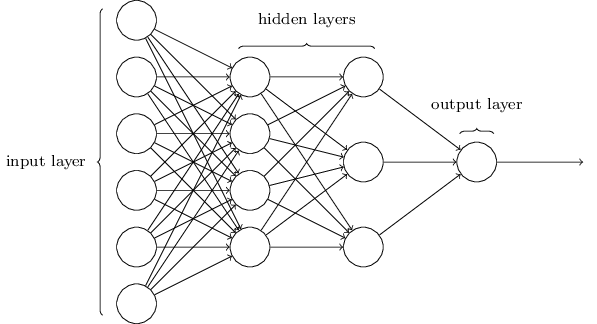
\includegraphics[width=0.25\textwidth]
    				{img/feedforward_architecture.png} 
    			}}%
    			\qquad
    			\subfloat[Convolutional]
    			{{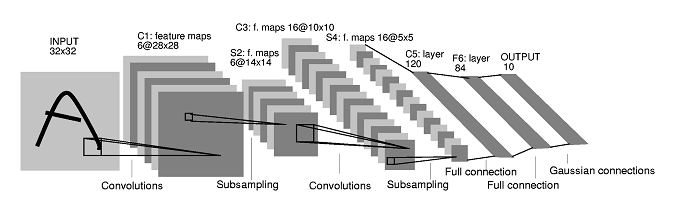
\includegraphics[width=0.45\textwidth]
    				{img/convolutional_architecture.png} 
    			}}%
    			\caption{Two of the most common architectures used for DNNs}%
    			\label{fig:architectures}
		\end{figure}		 		
		 		
		ANNs consist of a series of layers. These layers are composed of artificial `neurons' that compute a function on the inputs provided by the previous layer. They then pass the results (activations, that are typically real-valued numbers in the range [0,1]) as outputs to deeper layers. Within any individual layer there exists only one type of neuron computing the same function: these neurons are differentiated by potentially distinct inputs, outputs and weight distributions. Layers themselves are defined by the number and pattern of connections between these neurons. 
		\par 
		In order for a network to perform its task, a neural network must first be trained. This involves modifying the weights and biases of the network such that it produces the correct response for each of a number of training examples. The activations of the input units are set according to the feature values of the example, then these are propagated through the network to the output units, where the result is compared to the target output for that example and an error value calculated. This error signal is then back propagated through the network until the weights of the network have reduced the error at each connecting node. The changes that occur are typically very small, and so large training sets are required to successfully converge the network on an optimal weight distribution.
		\par 
		The intuition behind back propagation, the algorithm that adjusts the weights with respect to the error value, is one of assigning `blame'. The activations of the output nodes are determined by the activations of all the nodes below it, therefore error at the output is a result of the weights acting directly upon it from the preceding layer, and those recursively before it. In order to adjust the weights lower-down the error is backwardly propagated to the lowest hidden nodes that contributed an poor activation.		
		\par
		This process amounts to inductively learning how to solve a problem by exploiting regularities across a training set so that future similar examples may be classified in the same way. This is very similar to the way a human child learns.

	\subsubsection{Layers}

		\begin{figure}[H]
    			\centering	
    			{{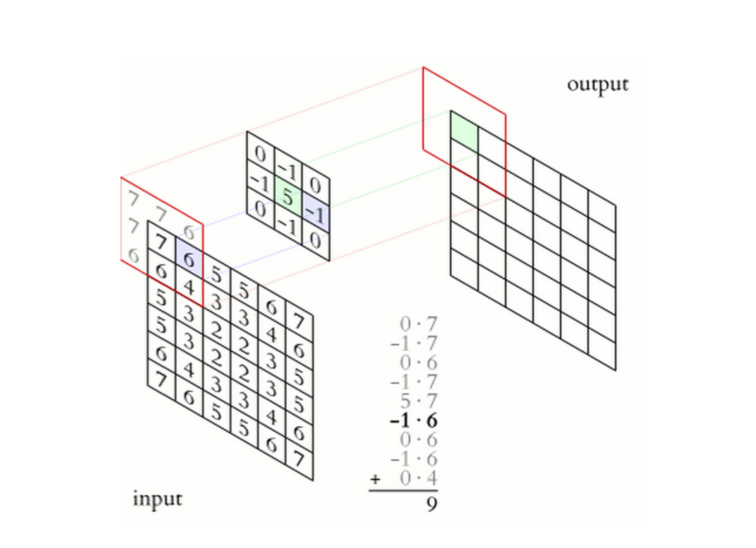
\includegraphics[width=0.45\textwidth]
    				{img/convolutional_network.png} 
    			}}%
    			\caption{Convolutional Filters}%
    			\label{fig:convfilters}
		\end{figure}		

		\par 
		There are a number of different types of layers that can be combined in a neural network: in a \textit{fully connected layer} the neurons receive an input value from every neuron in the previous layer. In a \textit{locally connected layer} the neurons are indexed spatially with inputs coming only from those nearby, and in a \textit{convolutional layer} a number of filters are applied to create a convolution. 
		\par
		The convolution of an image is produced by applying a filter upon the input image. The filter is a $k \times k$ weight matrix such that $ k $ is an odd number to ensure the matrix has a true centre. The convolved image is produced pixel at a time by computing the dot product of the filter and the pixels below it, the central pixel of which is updated. A convolution is therefore produced by scanning the filter across the input pixel space until every pixel is replaced by a pixel that is some function of its filter bound neighbours. Deep successions of convolutions encode images in ways that make them invariable to translation and deformation. This is critical for classification \cite{Bruna2012}.

\subsubsection{Neurons}
		
		\begin{figure}[H]
    			\centering	
    			\subfloat[Multipolar Biological Neuron]												{{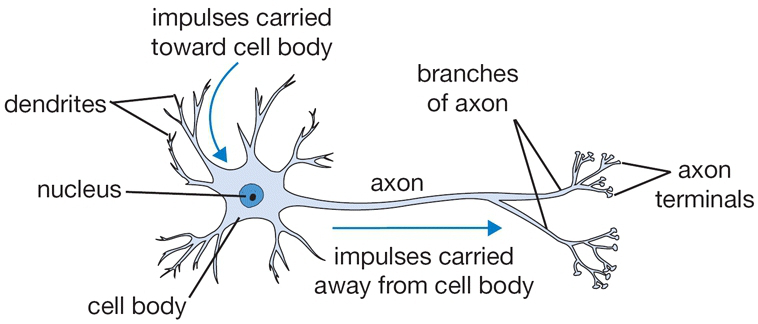
\includegraphics[width=0.3\textwidth]
    				{img/neuron_bio} 
    			}}%
    			\qquad
    			\subfloat[Artificial Neuron Model]
    			{{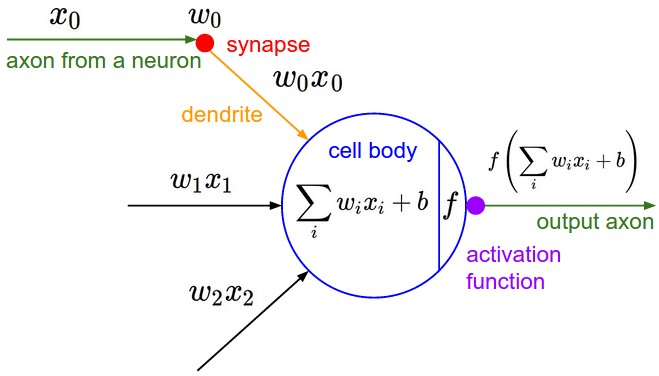
\includegraphics[width=0.3\textwidth]
    				{img/neuron_model} 
    			}}%
    			\caption{ }%
    			\label{fig:biologicalNeurons}
		\end{figure}
				
		As mentioned previously, artificial neural networks are loosely modelled on the human brain, and take influence from the \textit{multipolar biological neuron}. The neuron receives multiple electric charges from its neighbours through the dendrites. This then triggers a single electric charge to a different set of neighbouring neurons through its axon terminals. Artificial neurons perform effectively the same task and compute functions that take in multi-dimensional input but output a mono-dimensional result.
\\

There are a number of different neurons used within the layers of an artificial neural network:
		\\\
		
		\textbf{Binary Threshold Neuron} 
		
		$$
		y = \begin{cases}
		1 & \text{if \textit{M} $\le \sum\limits_{i=1}^k x_{i} \cdot w_{i} + b $ where \textit{M} is a threshold parameter} \\
		0 & \text{otherwise.}
		\end{cases}
		$$

		Here, \textit{y} is the output of the neuron calculated by the weighted input acting upon it, and assessing this value against some threshold \textit{M}. The threshold neuron works much like a biological neuron in that it either outputs a charge or it doesn't. This neuron however is rarely used due to the fact that it breaks optimisation algorithms, such as gradient descent, which require a function to be differentiable. 
	\\\

		\textbf{Logistic Sigmoid Neuron}	
		
		$$
		y = 
		\text{ $ \frac{1}{1 + \exp (-z)} $
		, where z = $ \sum\limits_{i=1}^k x_{i} \cdot w_{i} + b $}
		$$ 
		
		A commonly used transfer function is the sigmoid, which is a differentiable approximation of the threshold function above. Here the bias $ b $ performs a similar function to the threshold \textit{M} in the previous example. The `threshold' can be through of as the point at which the gradient of the \textit{decision surface} is steepest. While in the threshold neuron this represents a hard boundary, the sigmoid represents a gradient of values. One disadvantage of the sigmoid is that is is more expensive to compute.
		
		\begin{figure}[H]
    			\centering	
    			\subfloat[Sigmoid A]																			{{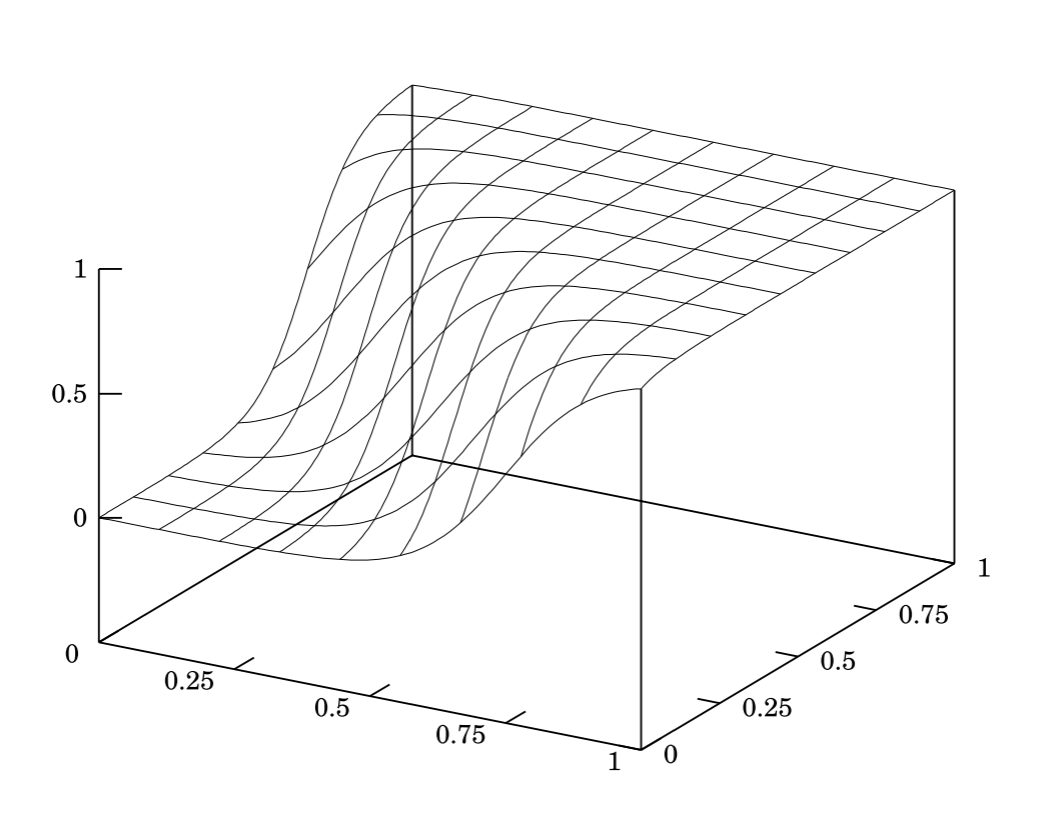
\includegraphics[width=0.2\textwidth]
    				{img/craven_sigmoid.png} 
    			}}%
    			\qquad
    			\subfloat[Threshold]																			{{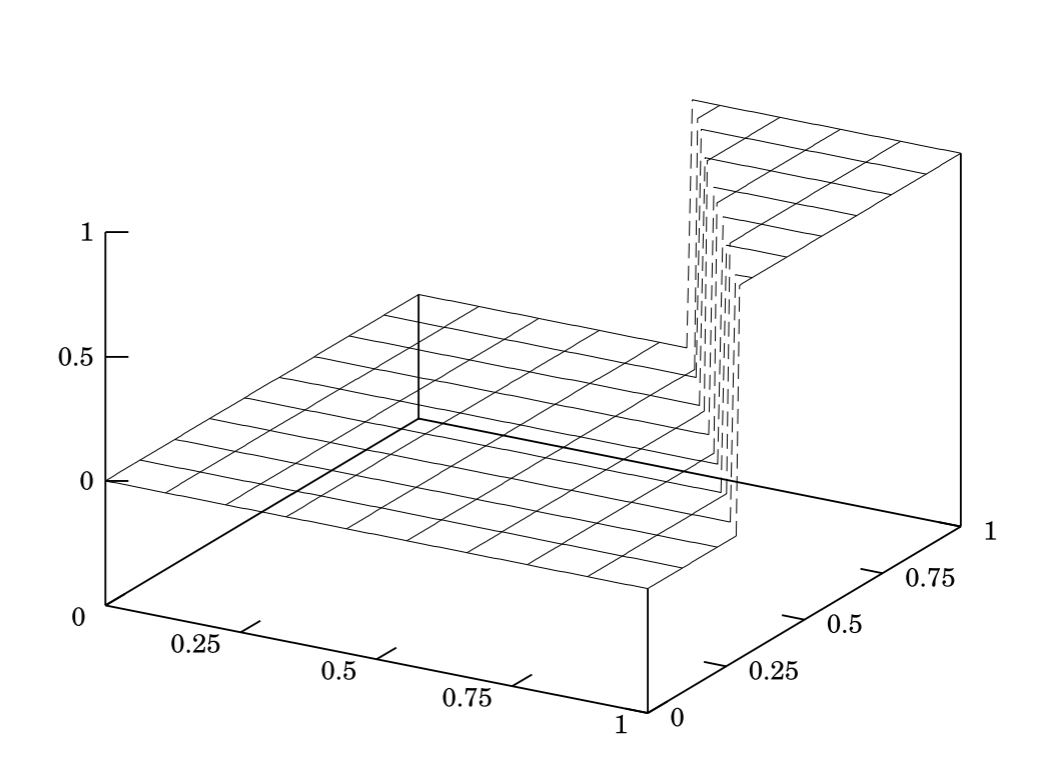
\includegraphics[width=0.2\textwidth]
    				{img/craven_threshold.png} 
    			}}%
    			\qquad
    			\subfloat[Sigmoid B]
    			{{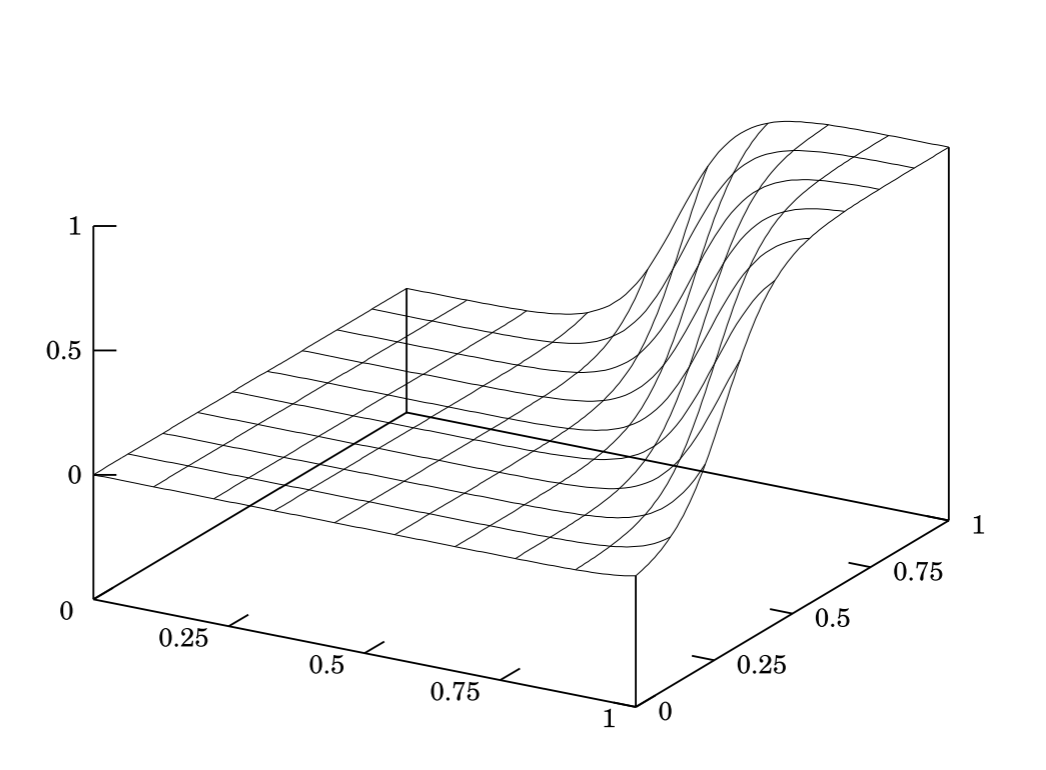
\includegraphics[width=0.2\textwidth]
    				{img/craven_sigmoid_2.png} 
    			}}%
    			\caption{}%
    			\label{fig:SigmoidNeurons}
		\end{figure}

		\textbf{Rectified Linear Neuron (ReLU) }
		
		$$
		y = 
		\text{ max$\{0,  b + \sum\limits_{i=1}^k x_{i} \cdot w_{i}\}$ }	
		$$		
		
		The rectified linear neuron is a hybrid function. It is more efficient to compute than the sigmoid neuron and is partially differentiable, thus making it suitable for gradient descent. The compromise here is the cost of sophistication of the result.

\subsubsection{Design Space}
		In a typical machine learning workflow, including working with ANNs, practitioners iteratively develop algorithms by refining choices in areas such as feature selection, sub-algorithm selection, parameter tuning and more \cite{Patel2008}. This is usually done through a trial and error approach that is perhaps similar to hill-climbing in the model space and can likewise lead to locally minimal results.
						
		\begin{figure}[H]
    			\centering	
			{{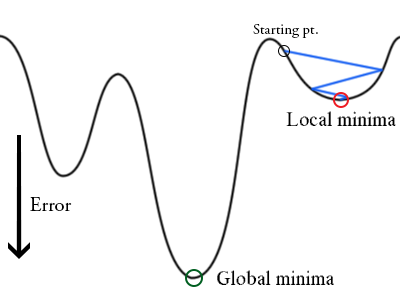
\includegraphics[width=0.3\textwidth]
    				{img/gradient_descent.png} 
    			}}%
    			\caption{Hill Climbing in the parameter space (Gradient Descent)}%
    			\label{fig:GradDesc}
		\end{figure}	
		
		\par 
		Some examples of parameters that require tuning are:
		\par
		\textbf{Size of Filters:} if the filter is too small features will be too coarse, however if the filter is too large the complexity of a model increases significantly with little benefit.
		\par
		\textbf{Number of Layers:} additional layers tend to improve performance, however they also increase a models complexity and thus its training time - this means that fewer model iterations are possible within a set time period. Back propagation issues with layers failing to train can also arise.
		\par 
		\textbf{Filters per Layer:} additional filters likewise tend to improve performance, and again there is likely to be a cut-off point where diminishing returns are outweighed by increased model complexity and training time.
		\par  
		\textbf{Layer Connectivity:} variations in locally-connected and fully-connected layers can change performance dramatically, such as exhibited in the difference between convolutional layers, fully connected layers and those with dropout.
		\par 
		\textbf{Input and Output Data Encodings:} different vector encodings change the way the network learns. Images for example with a height, width and three colours per pixel are compressed into a one-dimensional vector used as input.
		\par  		
		\textbf{Error Space, or Bound:} changes how the network perceives error, and thus fundamentally effects what it learns during the back-propagation optimisation period.
		\par		 		
		\textbf{Initialization of Weights:} can also alter how a model learns. There are a number of different possible approaches to this: such as uniformly, randomly, as a Gaussian, unsupervised pre-training and more. Initialisation can significantly effect error propagation: too low and error won't propagate and the network won't learn.
		\par 
		\textbf{Auxiliary Layers:} in ConvNets for example, pooling and normalization layers are often applied, however each has it's own set of additional parameters to tweak and a different effect on the model, thus requires complex tuning or remaining with common choice values.
		\par 
		\textbf{Non-linear functions:} can make a large difference on model performance: the choice of which non-linearity you choose, for example choosing a `Rectified Linear' neuron as opposed to a `sigmoid' as explained previously.
		\par 
		\textbf{Optimization Parameters:} such as step-size, or learning rate, regularisation, mini-batch sampling all need to be tuned for maximum accuracy and convergence speed. While there are common algorithms that help choose these parameters, such as AgaGrad \cite{Duchi2011}, manual tuning is often still required, and can be difficult to get right.
		\par
		\textbf{Momentum Co-efficient:} adds a fraction of the previous weight update to the current one, and is used to help prevent the system from converging to a local minimum or saddle point, and increase the speed at which it converges. Too high and risk of overshooting the minimum, and too low the system might still hit a local minima.
	\subsection{Black Box Problem}
		\subsubsection{Overview}
		While there have been some improvements to neural networks over the years, such as the development of drop-out, they remain to be considered by many as a black box algorithm \cite{Bernd1999}, especially in comparison to some other better studied and less complex machine learning techniques such as support vector machines or logistic regression. Indeed many popular machine learning competitions are still won by those better understood algorithms despite their comparative simplicity \cite{Adams2015}.
		\par 
		There is no clear understanding of why deep neural networks perform so well or why certain combinations of internal weights and connections enable highly complex tasks, such as computer vision, to be performed. Often as a result the development of new models falls largely upon a `greedy' trail and error approach to tuning the network parameters. This is unsatisfactorily unscientific, using experience and intuition as the primary guiding factors - making insights hard to replicate or teach.
		\par
		
		\begin{figure}[H]
    			\centering	
			{{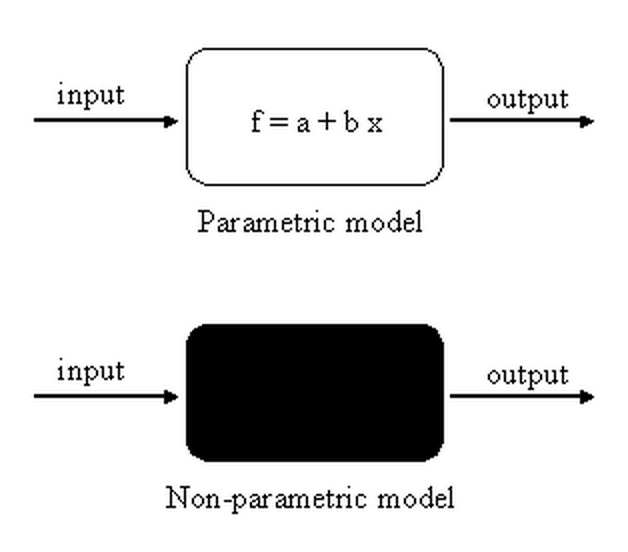
\includegraphics[width=0.25\textwidth]
    				{img/black_box.png} 
    			}}%
    			\caption{Black Box problem}%
    			\label{fig:BlackBox}
		\end{figure}	 

		\subsubsection{Existing Solutions}
		It is hoped that alternative work flows may provide deeper insight. \cite{Jarrett2009} for example uses a table of pre-evaluated models compared against a number of datasets in order to make more informed decisions. \cite{Bergstra2013} uses a less human involved approach by using Bayesian statistics to automate the search of the parameter space, this computationally demanding task neither always provides an optimal solution nor is it always possible.

\clearpage 

\section{Searching for a Solution}
	\subsection{Human \& Computer Augmentation}

\subsubsection{Solving Hard, Complex Problems in the Real World}

	When former world champion chess grandmaster Garry Kasparov was beaten by IBM’s deep blue in February 1996, the headline was that Artificial Intelligence had finally surpassed human intellect. However following that loss Kasparov founded a competition known as freestyle, or advanced, chess - here human chess players use software to augment their play. The results were significant: humans who teamed up with machines could beat any of the autonomous machines. So while AI is often heralded for its number crunching abilities, it's important to recognise that humans still bring important qualities to the intelligence scene. In short, intelligence augmentation of humans with computers is still superior to computer artificial intelligence.
	
		$$
			\mathbb{IA} > \mathbb{AI}
		$$
	
Companies such as PayPal and Palantir use machines to process data and humans to analyse it - often through visualisations - to perform complex fraud detection tasks that would be impossible for either to solve alone. By using the computer as a lever to analyse large datasets of neural network output through visualisation, this project hypothesises that the human-computer hybrid approach to understanding deep neural networks will be more successful than those purely computational methods described earlier.
	\par 
	It's important to stress here that this is not a novel idea, and similar projects have been undertaken across a variety of areas within Machine Learning, in the visualisations of the naive-Bayesian network \cite{Becker2001}, decision trees \cite{Ankerst1999}, Support Vector Machines \cite{Caragea2001} and Hidden Markov Models \cite{Dai2008}. Studies have shown that integrating visualisation tools into the learning work flow can in fact produce better results than automated techniques alone \cite{Ware2002}.

		\begin{figure}[H]
    			\centering	
			{{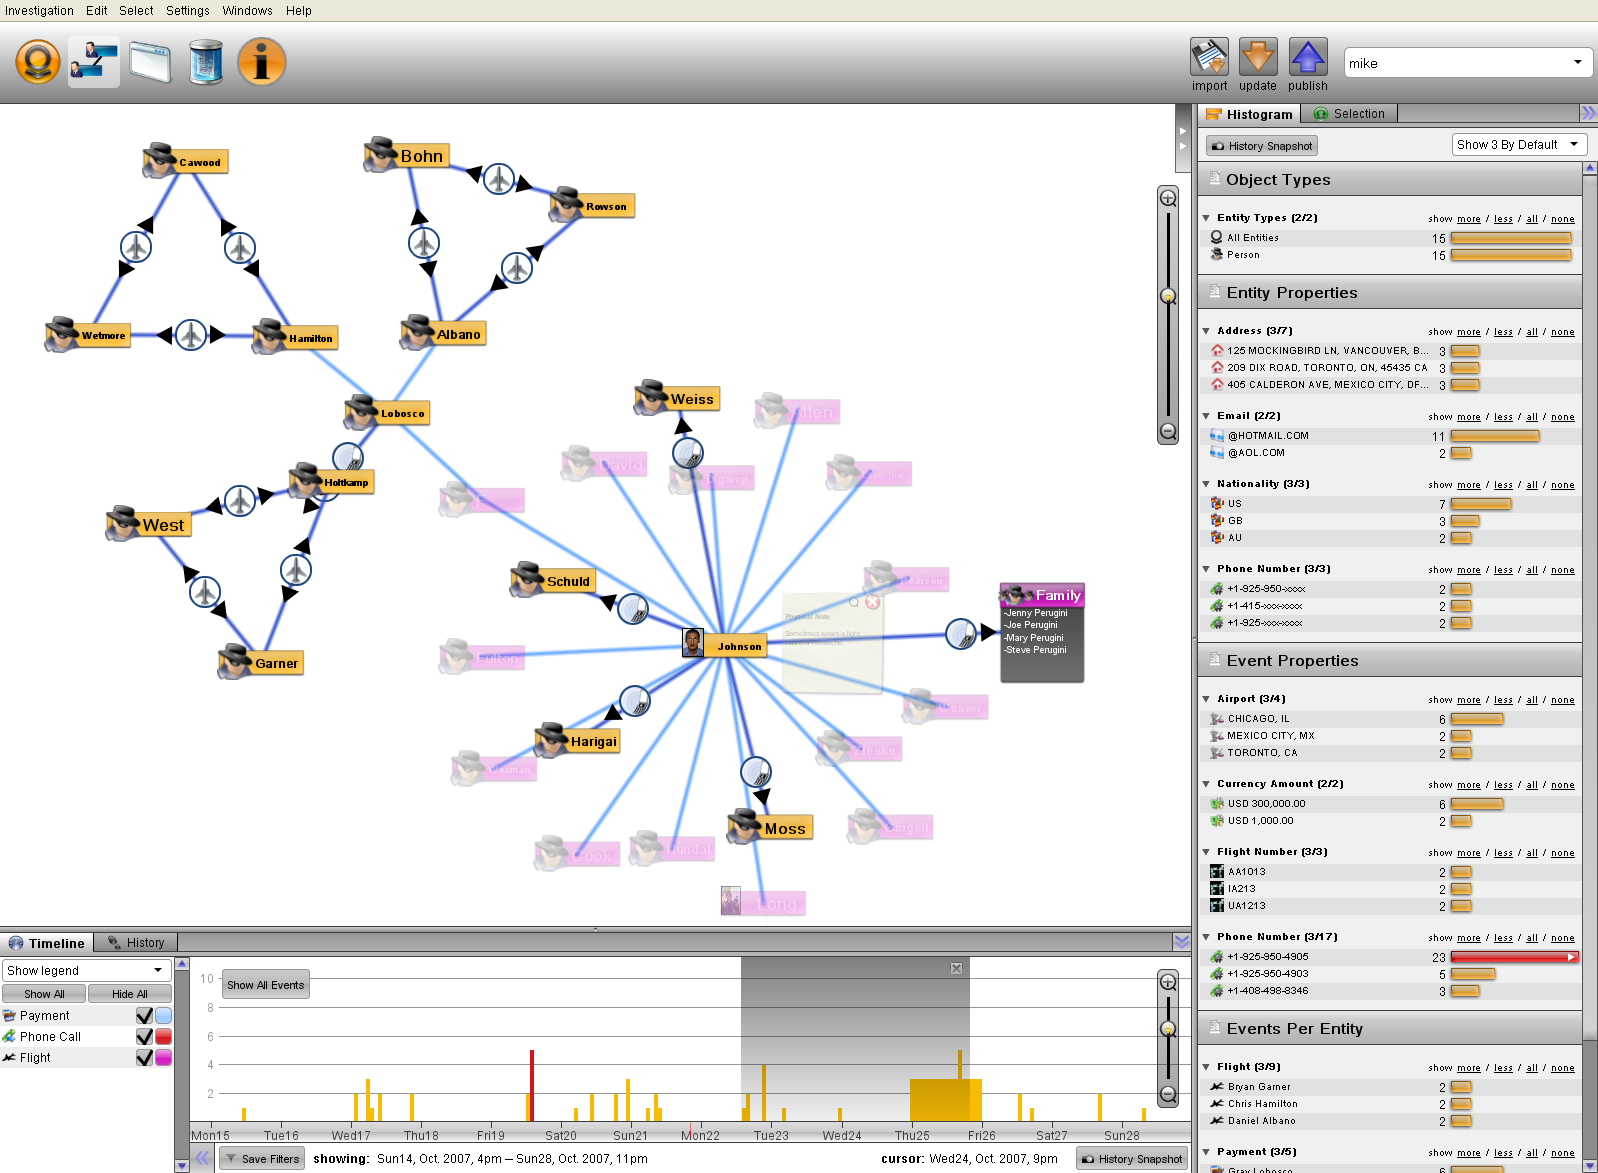
\includegraphics[width=0.4\textwidth]
    				{img/palantir_01.png} 
    			}}%
    			\caption{Palantir Visualisation tool: Humans augmented by computers}%
    		\label{fig:Palantir}
		\end{figure}

\textit{``The use of computer-supported, interactive, visual representations of abstract data can amplify cognition" \cite{card1999}}.


\subsubsection{Active Vision \& Problem Solving}
 	Using visualisation to augment intelligence is part of a small revolution in our understanding of human perception, sometimes called `active vision' \cite{Ware2010}. Active vision means that graphic designs and visualisations as more than pretty images, but should be seen as cognitive tools that enhance and extend our brains. Diagrams, maps, web pages, information graphics, visual instructions, and more regularly help us to solve problems through a process of visual thinking, using the enormous proportion - almost half - of the human brain that is devoted to the visual sense.  
 		
		\begin{figure}[H]
    			\centering	
			{{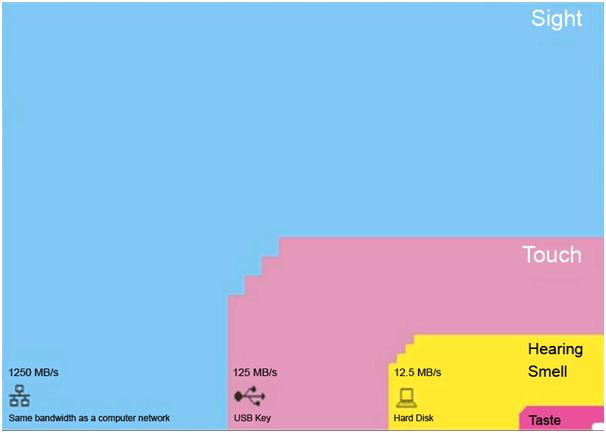
\includegraphics[width=0.3\textwidth]
    				{img/brain_bandwidth.png} 
    			}}%
    			\caption{Tor Nørretranders Brain Bandwidth}%
    		\label{fig:TufteExcellence}
		\end{figure}
		
		\par 
		Danish Physicist Tor Nørretranders discusses the ``bandwidth of our senses ” indicates the power of our visual systems. In the diagram the small white box at the corner is \textit{0.7\%} of total power and is what human beings are aware off when all this processing is happening \cite{Tufte2012}.		
		\\\
		\par 
		\textit{``We are all cognitive cyborgs in this Internet age in the sense that we rely heavily on cognitive tools to amplify our mental abilities. Visual thinking tools are especially important because they harness the visual pattern finding part of the brain."} \cite{Ware2010}.


	\subsection{Visualisation Theory}
	\subsubsection{Overview}
	Visualising quantitative information typically involves displaying measured quantities - data - by means of the combined use of points, lines, coordinate systems, numbers, symbols, words, shading, and/or colour. These visual forms are easily understood and an enable critique of in depth information underlying them \cite{DeFanti1989}, \cite{McCormick1987}, \cite{Tufte2001}.
		\par
		In numerical formats vast quantities of data can be tedious to process, and often little can be gained from such complex models. Visual data on the other hand communicates to the highly developed visual pattern-recognition capabilities of humans as already described. However there are a number of other details about this processing that are worth considering: images are pre-attentive and are processed before text in the human brain. Several empirical studies show that visual representations are superior to verbal or sequential representations across a number of different tasks; illustrating relations, identifying patterns, presenting overviews and details, supporting problem solving and communicating different knowledge types, and more \cite{Burkhard2004}. It is perhaps obvious that as a species humans are far better at recognising regularities, anomalies, and trends in \textit{images} rather than in long lists of numbers \cite{Ware2010}. Consider how difficult is may be to observe both global and local patterns in a list of numbers, in comparison to the relative ease when presented in a standard visualisation model such as a graph.
		\par 
		For data analysis to be truly effective, it is important to include the human in the data exploration process and combine the flexibility, creativity and general knowledge of the human with the enormous storage capacity and computation power of computers.
			  		 
  		\begin{figure}[H]
    			\centering	
			{{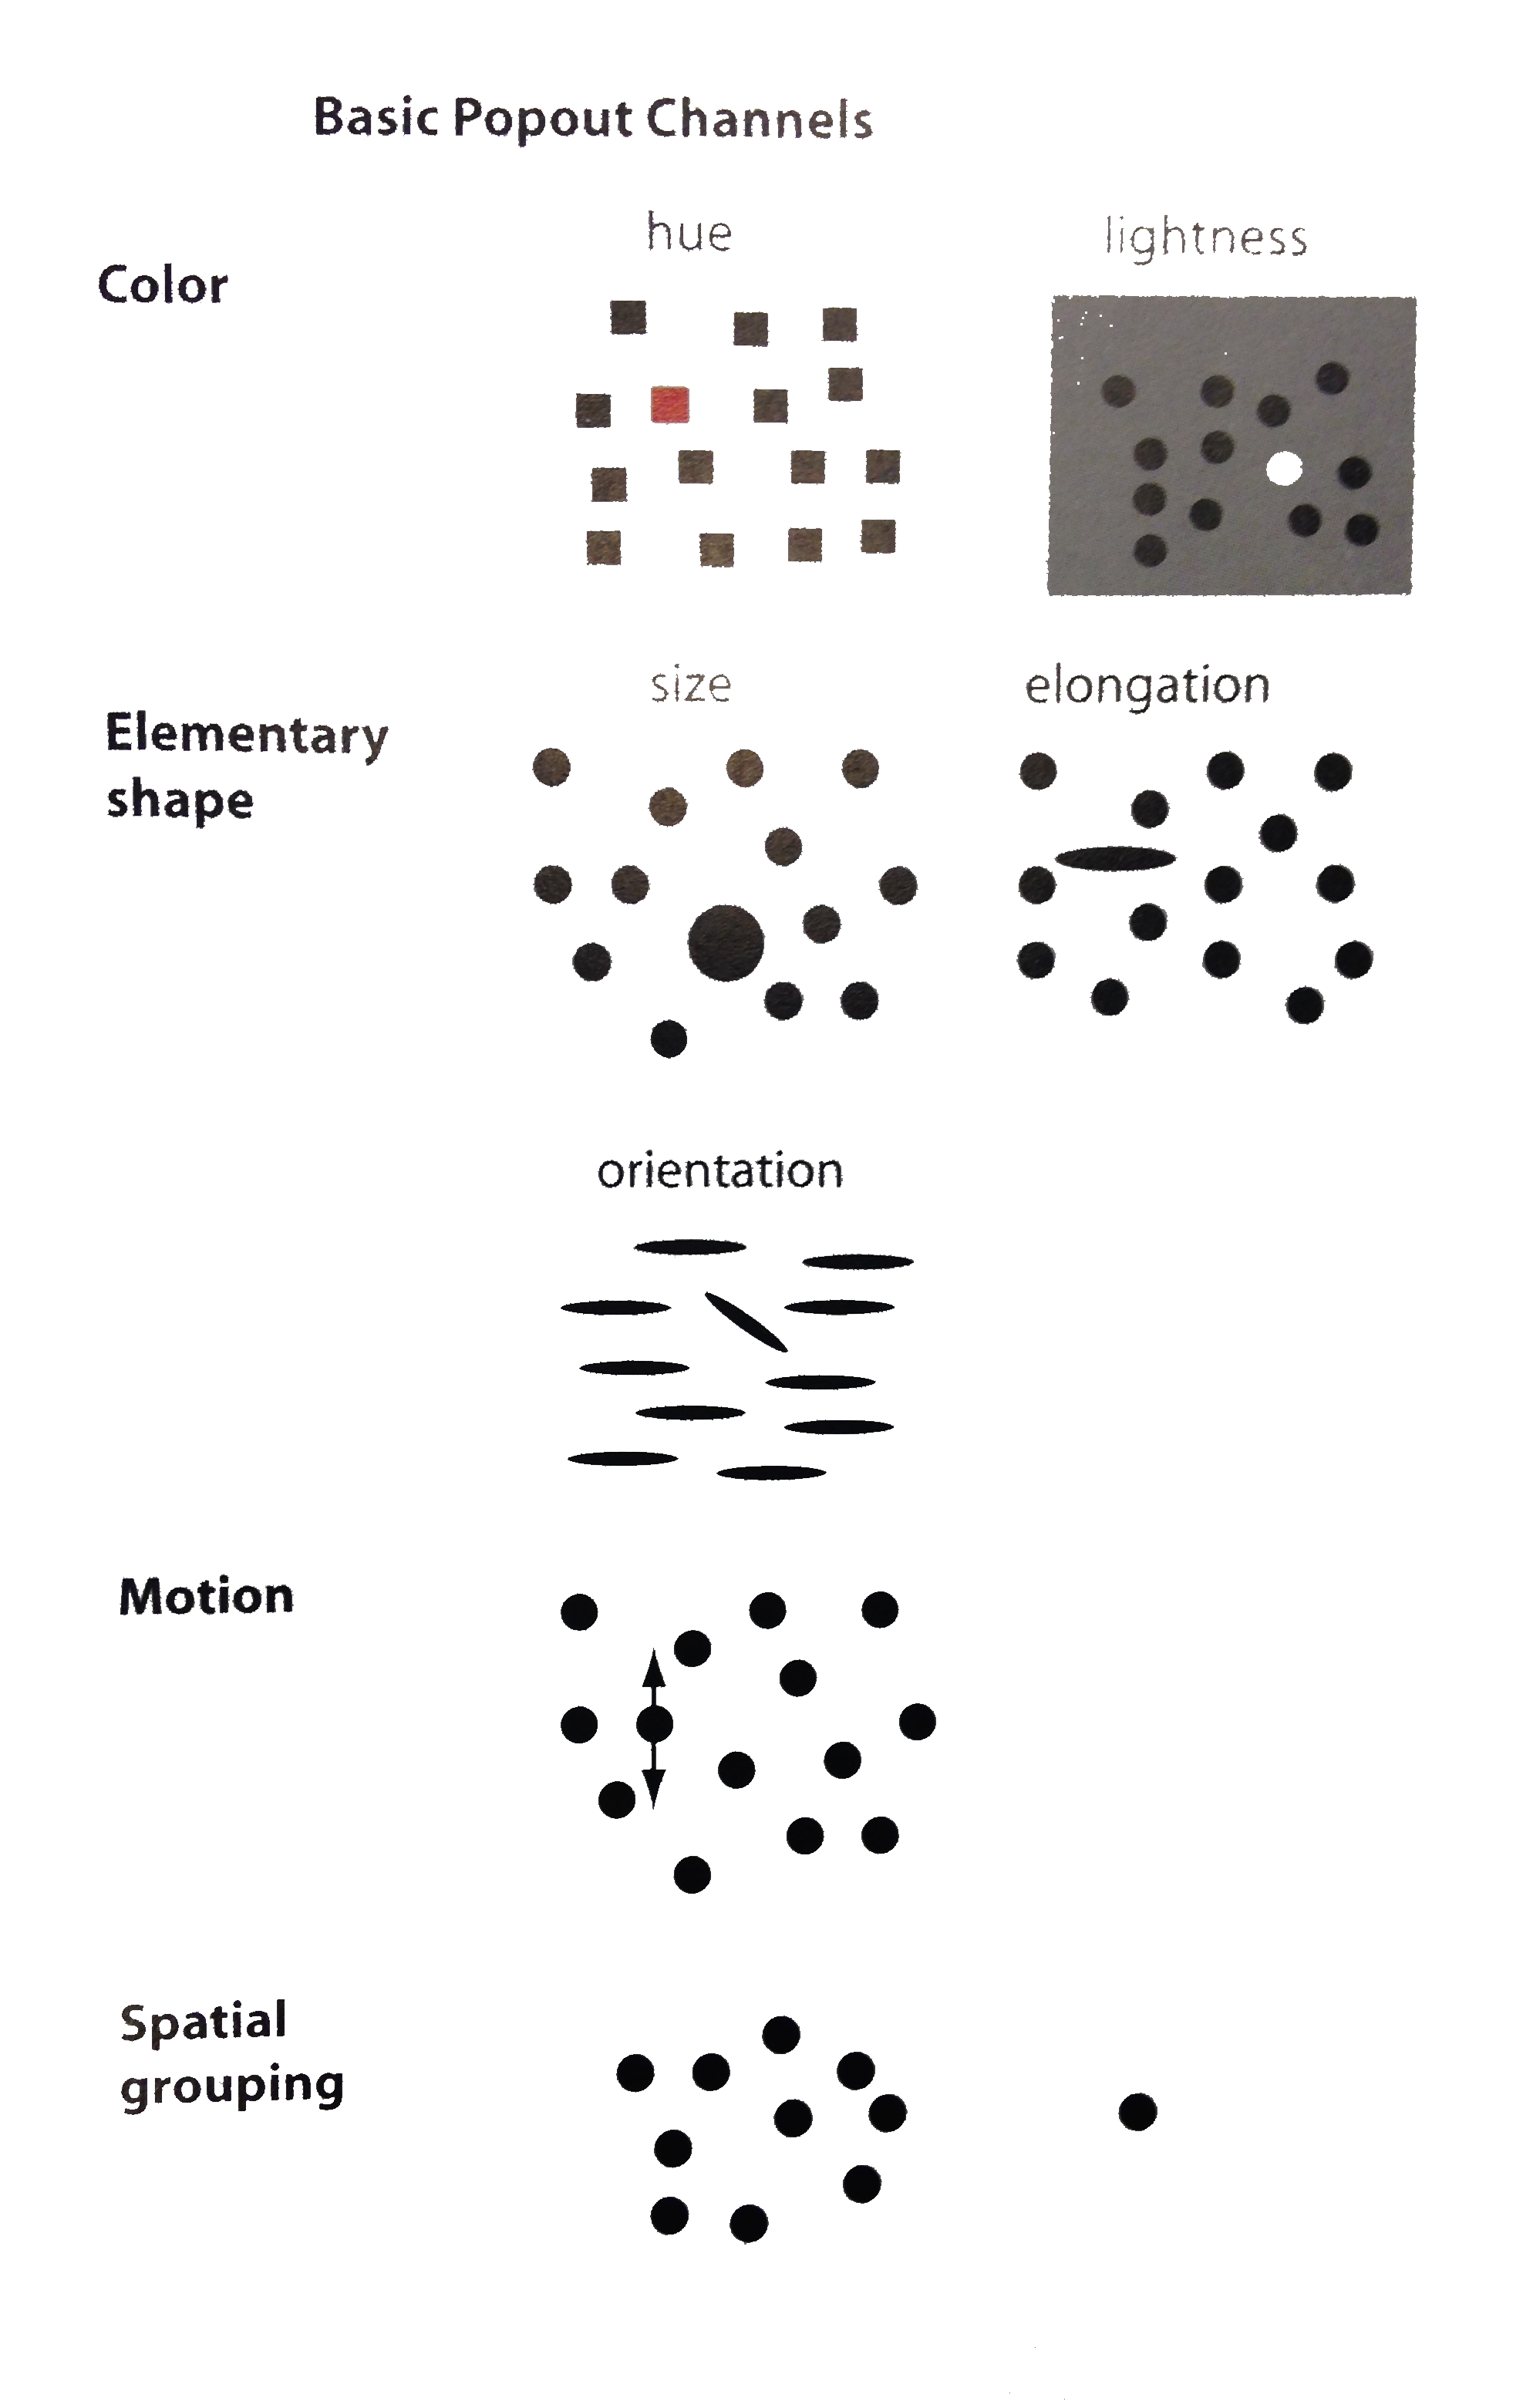
\includegraphics[width=0.4\textwidth]
    				{img/ware_popout_channels.png} 
    			}}%
    			\caption{Ware's ``Things that pop-out"}%
    		\label{fig:Ware Pop-Out}
		\end{figure}
		
		\par 
		Visual data exploration is especially useful when little is known about the data and the exploration goals are vague - such as with this task when attempting to understand the inner workings of a neural net. Since the user is directly involved in looking at the visualisation, shifting and adjusting the exploration goals of the human eye can be done automatically \cite{Keim2002}.
		\par 
		The canonical example of the usefulness of visualisation lies in the Anscombes quartet, where the four sets of numbers have many identical summary statistics - mean of x values, mean of y values, variances, correlations and regression lines - but vary wildly when graphed \cite{Shoresh2011}:

		\begin{figure}[H]
    			\centering	
				{{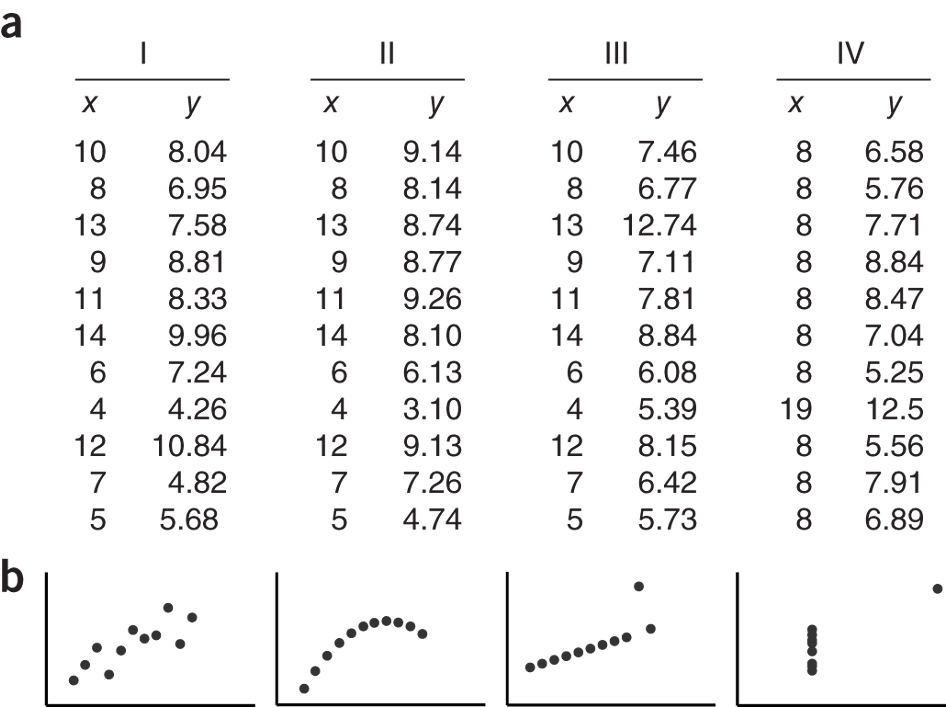
\includegraphics[width=0.5\textwidth]
    				{img/anscombes_quartet} 
    			}}%
    			\caption{(a) The four sets of numbers that form Anscombe's quartet -  (b) The highly distinctive graphs that result from plotting the data in a.}%
		\end{figure}


%\subsubsection{Tufte: what makes a good visualisation}

\subsubsection{Tufte's Rules}
		\par 
		All of this theory makes a clear argument to use visualisation, but in order to do this a set of practical guidelines must be explored. Edward Tufte, the founding father of data visualisation, provides us with a set of basic commandments \cite{Tufte2001}:		

		\begin{figure}[H]
    			\centering	
    			\subfloat[Poor Line Weights: unclear]												{{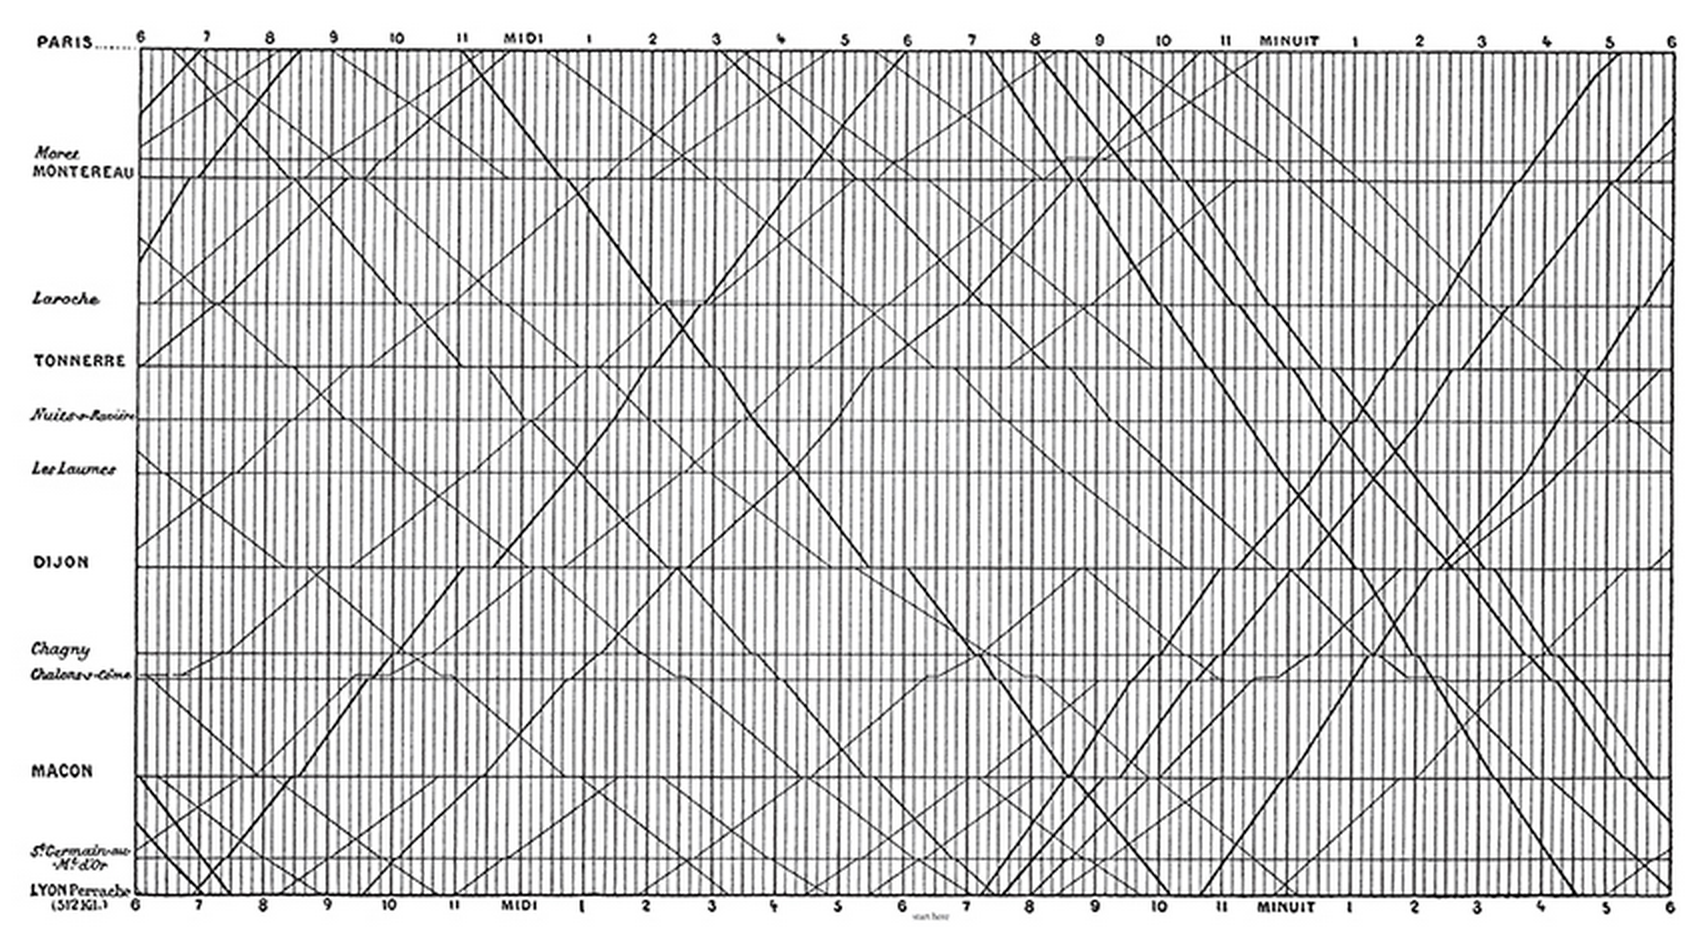
\includegraphics[width=7cm]
    				{img/marey_train_bad.png} 
    			}}%
    			\qquad
    			\subfloat[Better Line Weights: clear]
    			{{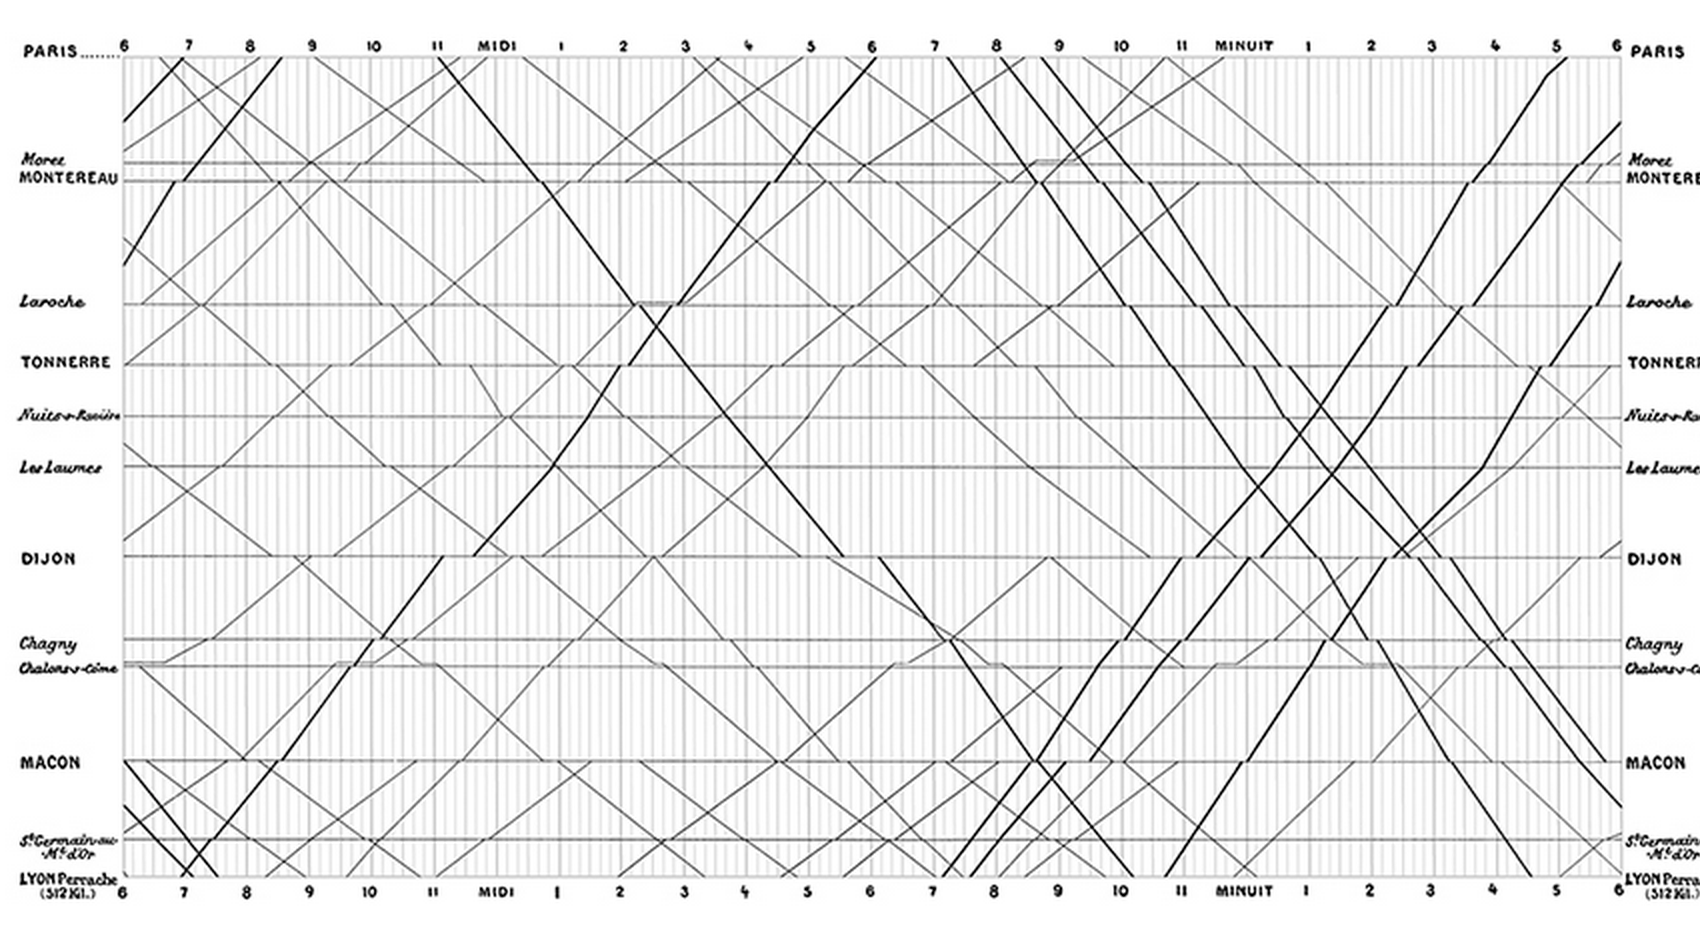
\includegraphics[width=7cm]
    				{img/marey_train_better.png} 
    			}}%
    			\caption{Tufte's train line chart demonstrating excessive data-ink}%
		\end{figure}

		\par
	\begin{itemize}
		\item \textbf{Principle One:}
		\textit{show only as much information as is required}
		\par 
		This is Tufte's \textit{data-ink} principle - irrelevant content is distracting, so should be removed. It is common place today to find charts and graphs with all sorts of three dimensional effects, unwanted background images and colours. The idea of having a data-ink ratio is to show only as much information as is required.
		$$
		\text{Data-ink ratio} = 
		\frac{\text{data-ink}}{\text{total ink used to print the graphic}}
		$$

		\item \textbf{Principle two:}
		\textit{include visual differences only when required} 
		\par
		The human brain has an amazing ability to spot visual differences such as color, size and position. Often our eyes look for the meaning to change depending on how these visual features are designed. If there is no difference, but embellishments are added, it often leads to confusion. He argues here for simplicity and clarity above all else.

		\item \textbf{Principle tree:}
		\textit{use visual encodings for quantitative values}
		\par 
		This is the key visual principle, successful examples of which are: length, for example the length of bar in a bar graph; 2-D location, for example the position of a data point in a scatter plot; size, for example the area in a pie chart; shape, orientation or hue, for example denoting different classes in any graph. All of these are automatically and immediate understood as they have natural properties that humans understand, far clearer than any numerical value.

		\item \textbf{Principle four:}
		\textit{differences in visual properties should correspond to actual differences in the data}
		\par 
		Its important to encode differences consistently and not manipulate the visualisation to aid an argument. For example, ensuring that axes are consistent - from zero to some useful value without undergoing any form of distortion.

		\item \textbf{Principle five:}
		\textit{do not visually connect values that are discrete}
		\par 
		In a graph, when you draw lines between discrete values and connect them, people perceive those values as having a relationship to each other. This should be avoided if no relationship exists.

		\item \textbf{Principle six:} \textit{visually highlight the most important part of your message}
		\par 
		All information on a chart may not be equal so they should direct a users attention to a particular part of the visualization by visually highlighting the data through the use of color, position or another standard encoding.

		\item \textbf{Principle seven:} 
		\textit{augment short term memory through visual patterns}
		\par
		The human brain is limited to retaining around four pieces of information at any given time. By presenting large pieces quantitative information as visual patterns, such as in plots, more information can be understood at any given point.
		
	\item \textbf{Principle eight:}
	\textit{Encourage the eye to compare different pieces of data}
	\par
	Information is not something that exists in isolation, and often by comparing pieces of information one is brought to new conclusions about that data.
	\item \textbf{Principle nine:}
	\textit{Reveal the data at several levels of detail}
	\par
	Quantitative data often has several scales, with patterns appearing at both a global and local level. By enabling the data to be viewed at different levels of detail the data can be explored in its full complexity.
	\item \textbf{Principle ten:}
	\textit{Don't distort the data:}
	\par
	Often it is tempting to change the scale on a graph for it to `fit' appropriately, or to crop the data hiding anomalies. With these elements of distortion the full picture is not revealed, and the purpose of visualisation compromised. 
	\end{itemize}
\subsection{Existing Neural Network Visualisations}
		
	Some of the principles described above have been adopted in neural net visualisations already, others have been ignored. This section explores some of these previous attempts at visualising networks which have been around helping researchers with neural networks for a long time, such as the \textit{Hinton diagram} were first demonstrated as early as 1986. This section provides a brief overview of similar techniques from around the nineties, where a number of the techniques are going to be visualisations of the simple neural network below.
	 
	 	\begin{figure}[H]
    			\centering	
			{{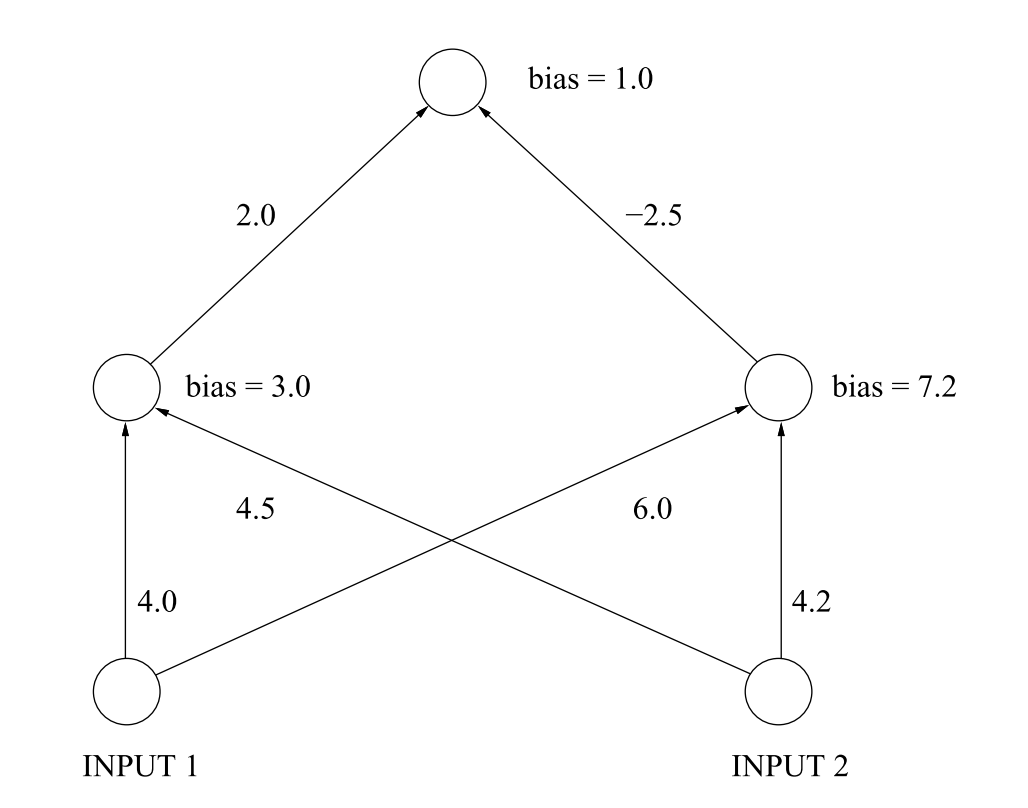
\includegraphics[width=0.4\textwidth]
    				{img/craven_simple_net.png} 
    			}}%
    			\caption{Simple Neural Network}%
    		\label{fig:simplenet}
	\end{figure} 	
		
%\subsubsection{Hinton Diagram}
\subsubsection{Hinton Diagram}

		 		
 	\begin{figure}[H]
    			\centering	
			{{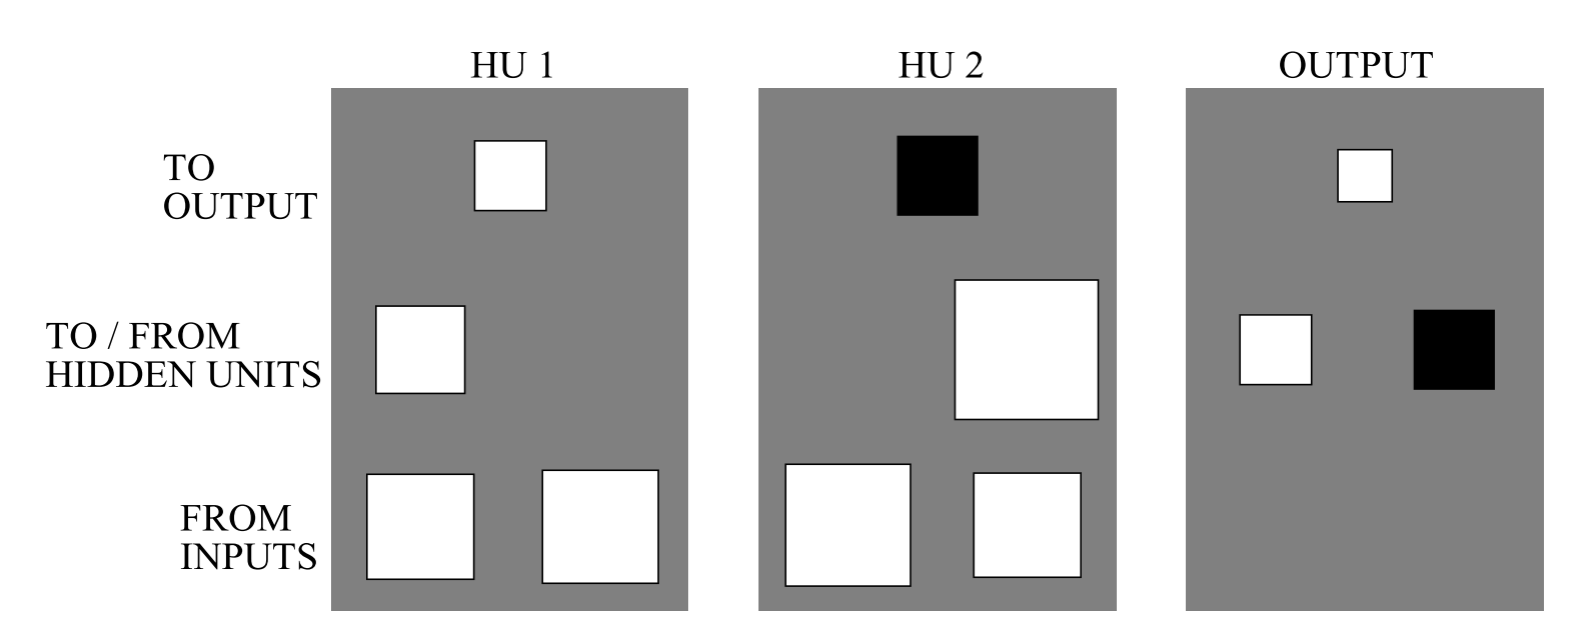
\includegraphics[width=0.4\textwidth]
    				{img/craven_hinton.png} 
    			}}%
    			\caption{Hinton Diagram}%
    		\label{fig:simple}
	\end{figure} 
 		
		One of the first practical visualisations of ANNs was the \textit{Hinton Diagram} \cite{Hinton1986}. It visualises the weights and biases relating to a node within a network. Weights are represented as boxes, where its area represents the weights magnitude, and it's shade represents the sign on the weight - white is positive, black is negative. Biases are illustrated as weights from a node back to itself. There is a vague representation of the architecture as output nodes appear at the top of a diagram, hidden nodes are in the middle, and input nodes are at the bottom. However these diagrams are rather unclear, and lack of topological information is a problem. The advantage is they make it easy to compare the signs and magnitudes of the weights that contribute to a neurons activation.
		\\\
		\\\
		
%\subsubsection{Bond Diagram} 
\subsubsection{Bond Diagram}		
 	\begin{figure}[H]
    			\centering	
			{{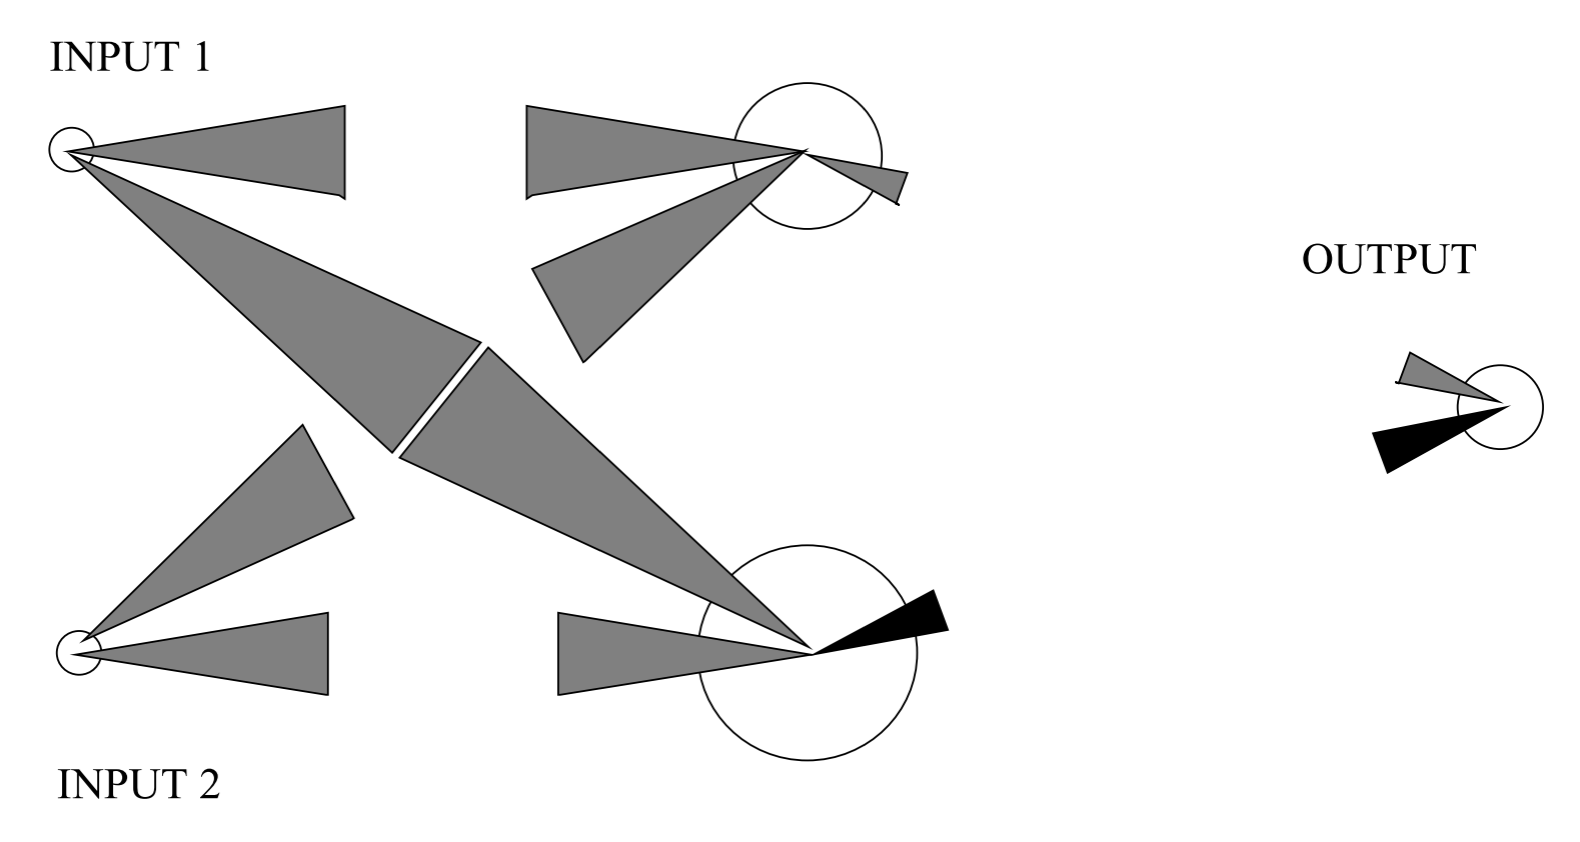
\includegraphics[width=0.4\textwidth]
    				{img/craven_bond.png} 
    			}}%
    			\caption{Bond Diagram}%
    		\label{fig:bond}
	\end{figure} 
 		
		Similar to the \textit{Hinton Diagrams}, the Bond diagram \cite{Wejchert1990} graphically depicts the values of the networks weights and biases. The bond diagram however attempts to make the architecture of the network more clear; a neuron is depicted as a circle, where the diameter of the circle indicates the magnitude of the bias, and triangles connecting the circles represent the weights. The magnitude is indicated by the height of the triangle, and colour depicts the sign. 
		\par 
		While it is perhaps easier to decipher the network structure from the Bond diagram, it is harder to gauge the relative importance of the weights and biases which have been depicted with different shapes. It makes the following question very difficult to answer: ``which input units need to be active in order for the net input to exceed the threshold (bias) of the hidden units?" \cite{Craven1992}, a useful question that Hinton diagrams are far better at answering.
		\par 
		
\subsubsection{Hyperplane Diagrams}
%\textbf{Hyperplane Diagrams}
		
 	\begin{figure}[H]
    			\centering	
			{{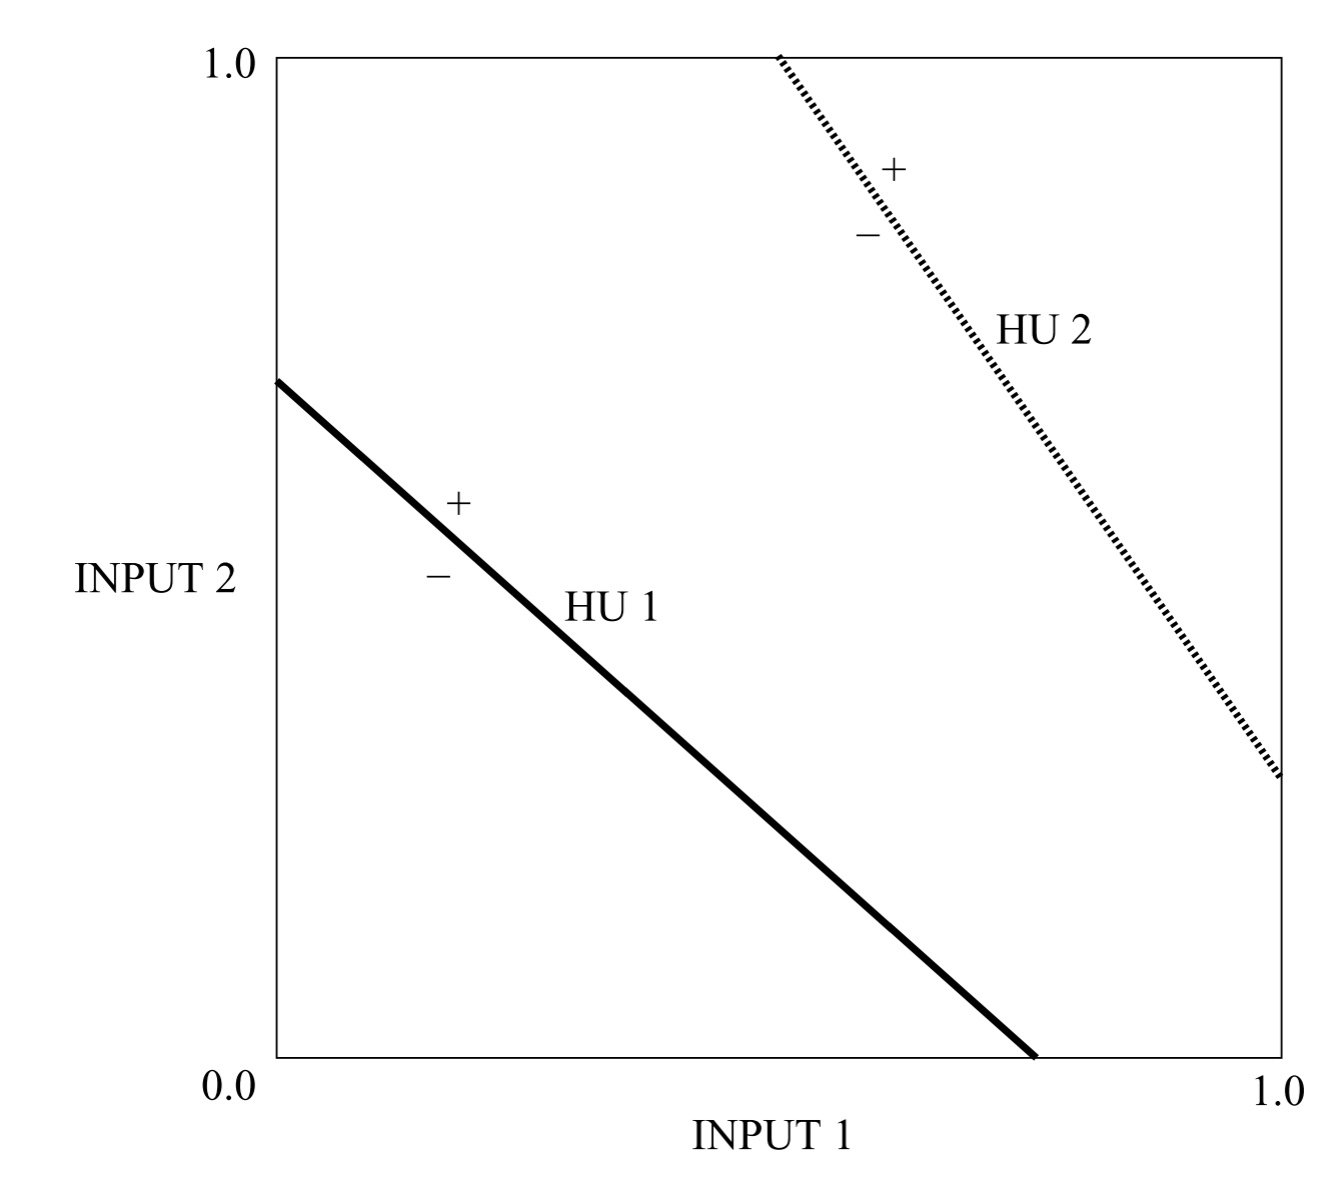
\includegraphics[width=0.4\textwidth]
    				{img/craven_hyperplane.png} 
    			}}%
    			\caption{Hyperplane Diagram}%
    		\label{fig:bond}
	\end{figure} 
 		
		A hyperplane depicts the `threshold' of a decision surface. As this hyperplane moves throughout the training process, visualising the hyperplane as it moves can be a useful method to get an understanding of what a neuron is learning \cite{Munro1992}. Neurons that appear in the same layer can have their hyperplanes shown in the same diagram due to a sharing of input space, making comparison easy.
		\par 
		One issue with this hyperplane representation is that while accurately representing a threshold function acting on a two-dimensional input space, the diagrams fall down when compared with most contemporary ANNs that require multiple dimensions ($>3$) to be shown and more commonly use continuous transfer functions such as  the sigmoid - which requires a gradual, rather than a sudden, division of the input space. That said, it can be assumed that the hyperplane is a close approximation of the gradual boundary and so can still provide useful observations.
		\par 
		
\subsubsection{Response-function plots}
%\textbf{Response-function plots}
		
 	\begin{figure}[H]
    			\centering	
			{{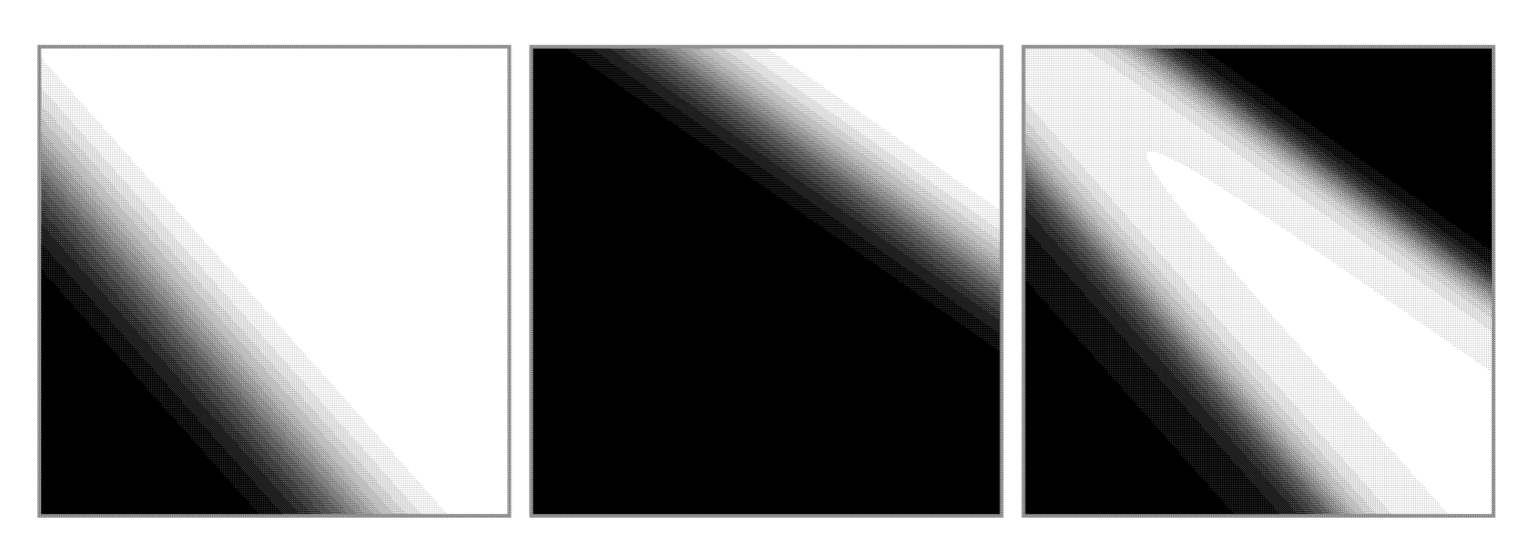
\includegraphics[width=0.4\textwidth]
    				{img/craven_gradient.png} 
    			}}%
    			\caption{Response Function Plot}%
    		\label{fig:bond}
	\end{figure} 
 		
		Response-function plots are very similar to hyperplane diagrams - they also display the decision surface. They differ in their solving of the issue of the gradual boundary. Instead of displaying the space using a hyperplane, the space is displayed as a gradient of values to indicate the resulting activations.
		\par 
		Interestingly, both the Response-Function Plots and the hyperplane diagrams show the space between two successive layers of neurons. This provides only a fraction of information about the network, and problematically may lead to false assumptions about it. One way to address this is to describe the decision surface not just on the layer below, but across all previous layers of the input space.
		\par 
		
\subsubsection{Trajectory Diagrams}
%\textbf{Trajectory Diagrams}
		
 	\begin{figure}[H]
    			\centering	
			{{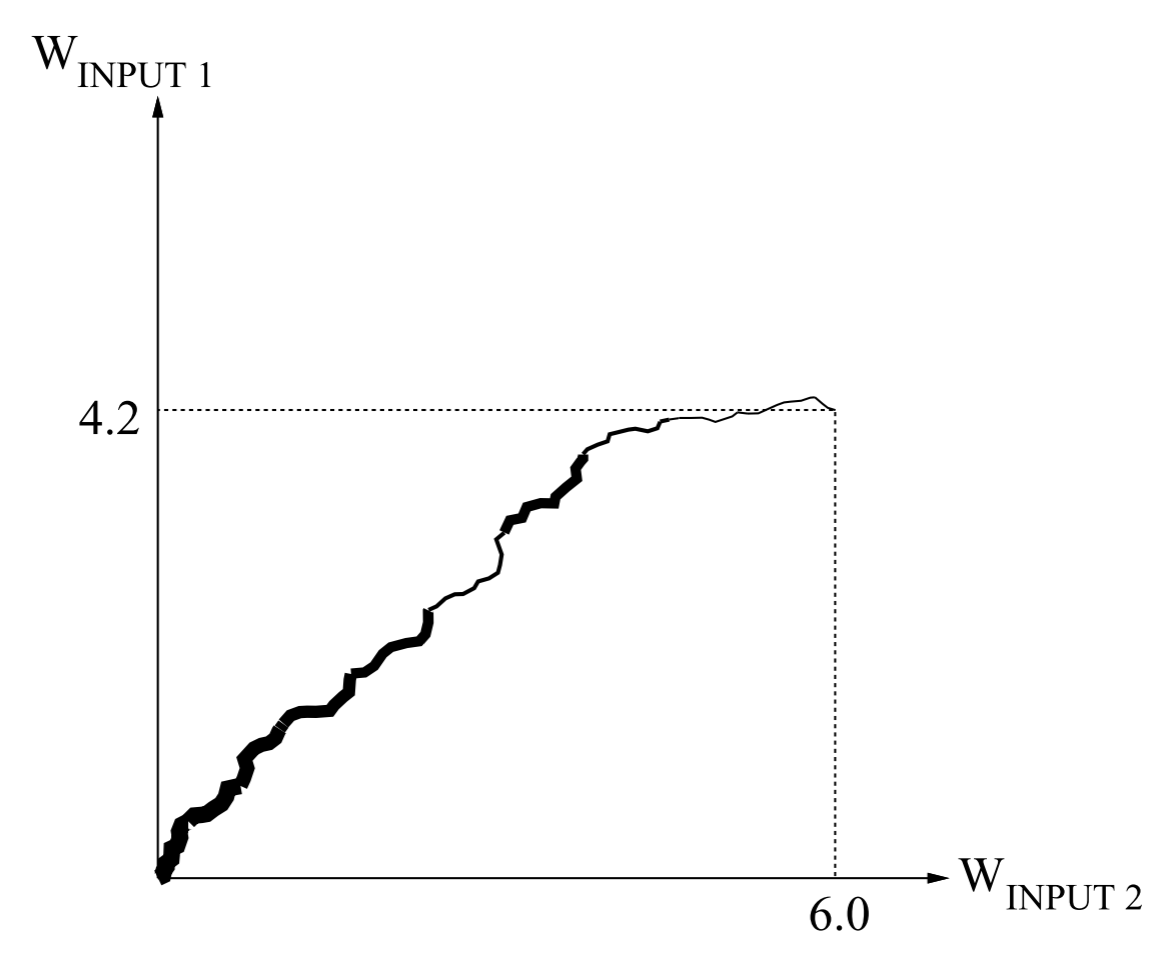
\includegraphics[width=0.4\textwidth]
    				{img/craven_trajectory.png} 
    			}}%
    			\caption{Trajectory Diagram}%
    		\label{fig:bond}
	\end{figure} 
 		
		Trajectory Diagrams \cite{Wejchert1990} depict the change in weight space and in error over a neuron during training. These diagrams use the incoming weights of a neuron to create the axes of a plot. During training as the weights change they are visualised as a trajectory in the weight space. The error at a given time is indicated by the thickness of the trajectory line.
		\par 	
		Again, along with many of these other early visualisation methods, the weakness of the trajectory diagram is its inability to display weight spaces of more than three dimensions. There have been efforts to combine dimensionality visualisation with trajectory diagrams - such as using radially projected axes, however this is fairly unsuccessful \cite{Craven1992}. 
		\par 
		
\subsubsection{Lascaux}
%\textbf{Lascaux}
		
	\begin{figure}[H]
    			\centering	
			{{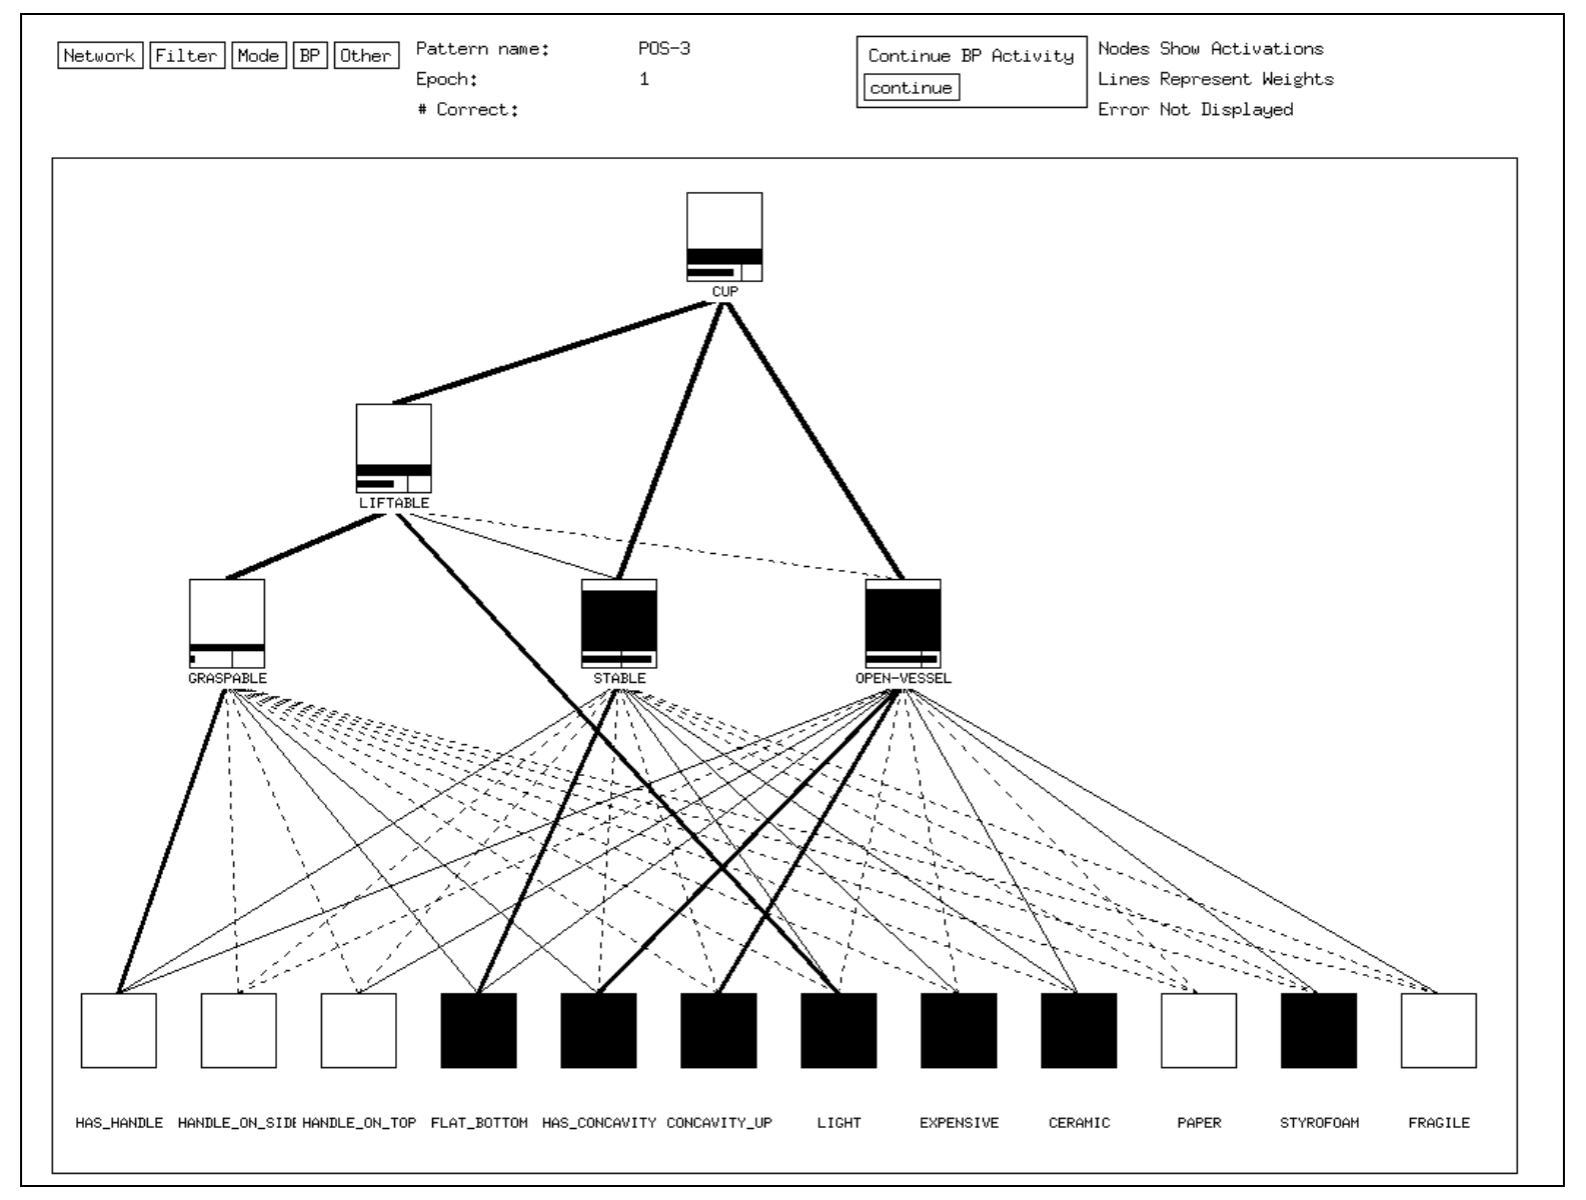
\includegraphics[width=0.4\textwidth]
    				{img/craven_weights.png} 
    			}}%
    			\caption{Lascaux Clip}%
    		\label{fig:lascaux}
	\end{figure}  		
 		
		Lascaux is a visualisation tool proposed by \cite{Craven1992} that aimed to clearly display the topology of a network. Here, each neuron is represented as a box and network weights are represented by interconnecting lines. A weights magnitude is visualised by the thickness of a line, and the positive or negative signs are visualised as solid and dashed lines respectively.
		\par 
		The tool depicts a range of information it one place. Activation of each neuron is show as a vertical bar within the neuron `box'; a horizontal bar shows the net input relative to a threshold - shown as a line intersecting the bar; error is another vertical bar within the neuron box; a separate diagram shows the error propagating as connections between these boxes - where thickness describes magnitude.
		\par 
		The issue with \textit{Lascaux} is that too much information is being displayed in a small space ineffectively. The approach uses standard two dimensional visualisation techniques, and simply squashes them into a neural network architecture. This makes the topology easier to understand, but at the sacrifice of more important elements.

\subsubsection{Tseng Map}
%\textbf{Visualising Weights and Connections}
		When representing weights, it is important to consider the analytical impact of a visual decision. \cite{Streeter2001} visualises the topology of the network but doesn't clearly show the weights themselves. This can lead to confusion when assessing the importance of a neuron. Consider for example a neuron that has appears to have a high value in one layer, however is subsequently cancelled out by low weights deeper within the network.
	\par 
	One problem here is that since the absolute values of the weights are used, the result does not provide the direction of the relationship. 
	\par 
		
	\begin{figure}[H]
		\centering 
    		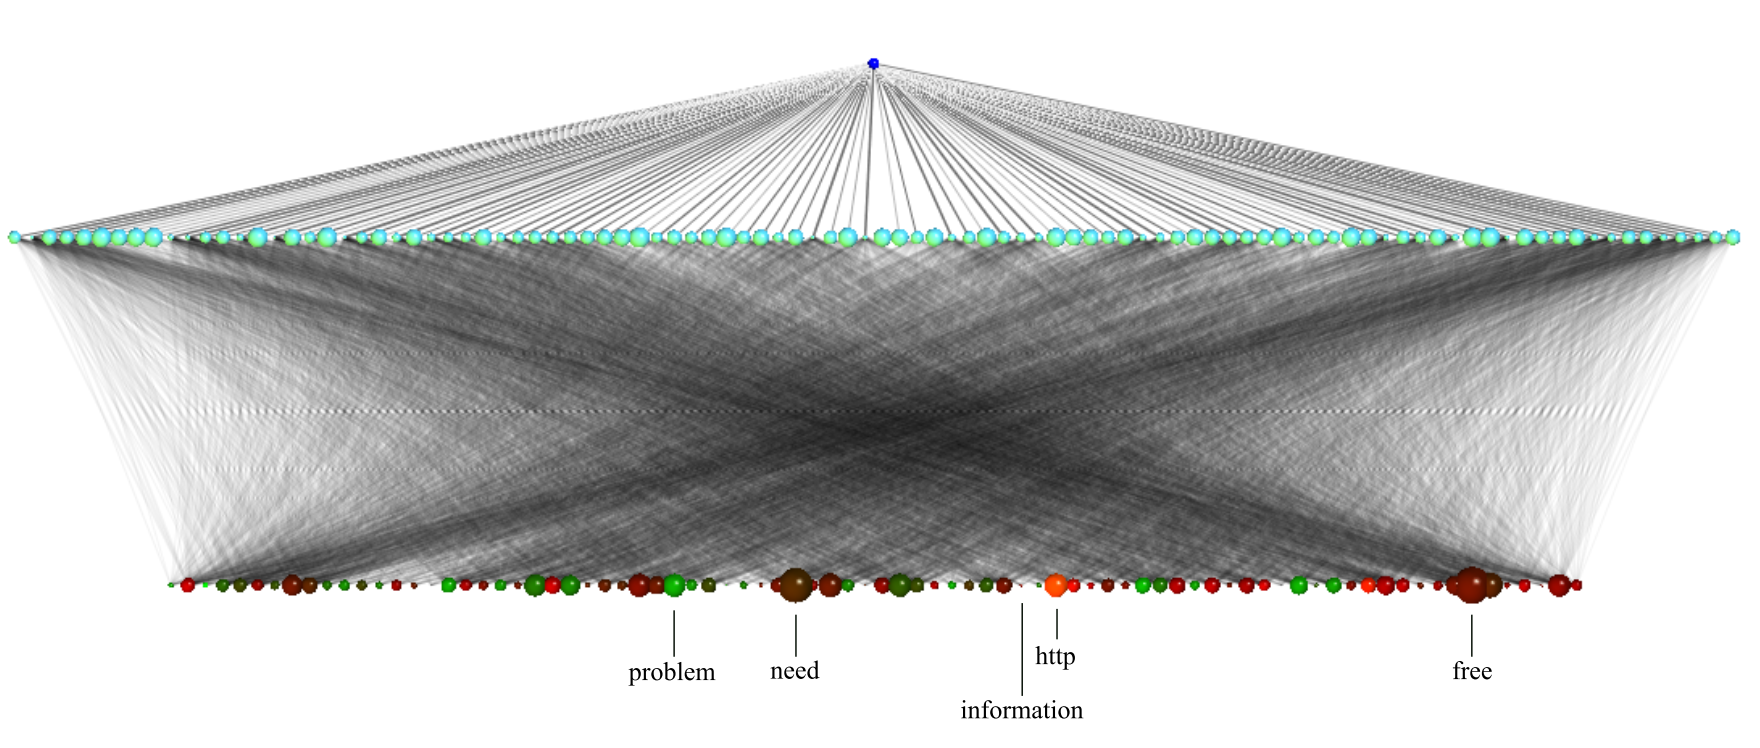
\includegraphics[width=0.7\textwidth]{img/tzeng_large_map.png} 
    		\caption{Tzeng Map}%
 	\end{figure}
 	
	\cite{Tzeng2005} based on the work of 	\cite{Garson1991} and \cite{Goh1995} sought to solve this problem in a different way; by visualising the weights with line-thickness between nodes, thus making it easy to identify when a node is insignificant regardless of the magnitude of weights applied to it. In addition 	\cite{Tzeng2005} propagate all of the layers influence through the network by multiplying each weight between the previous layers with those of the successive layers which connect to the same node.
	 
\subsubsection{Features}
%\textbf{Features}

		A more recent attempt at visualising neural nets is the feature mapping of convolutional neural networks. It is mostly limited to the simple visualisation of the 1st layer where projections to the pixel space are relatively easy to achieve. However there are exceptions, and a small number of researchers have developed methods for visualising deeper hidden layers.
		
		\begin{figure}[H]
			\centering	
    			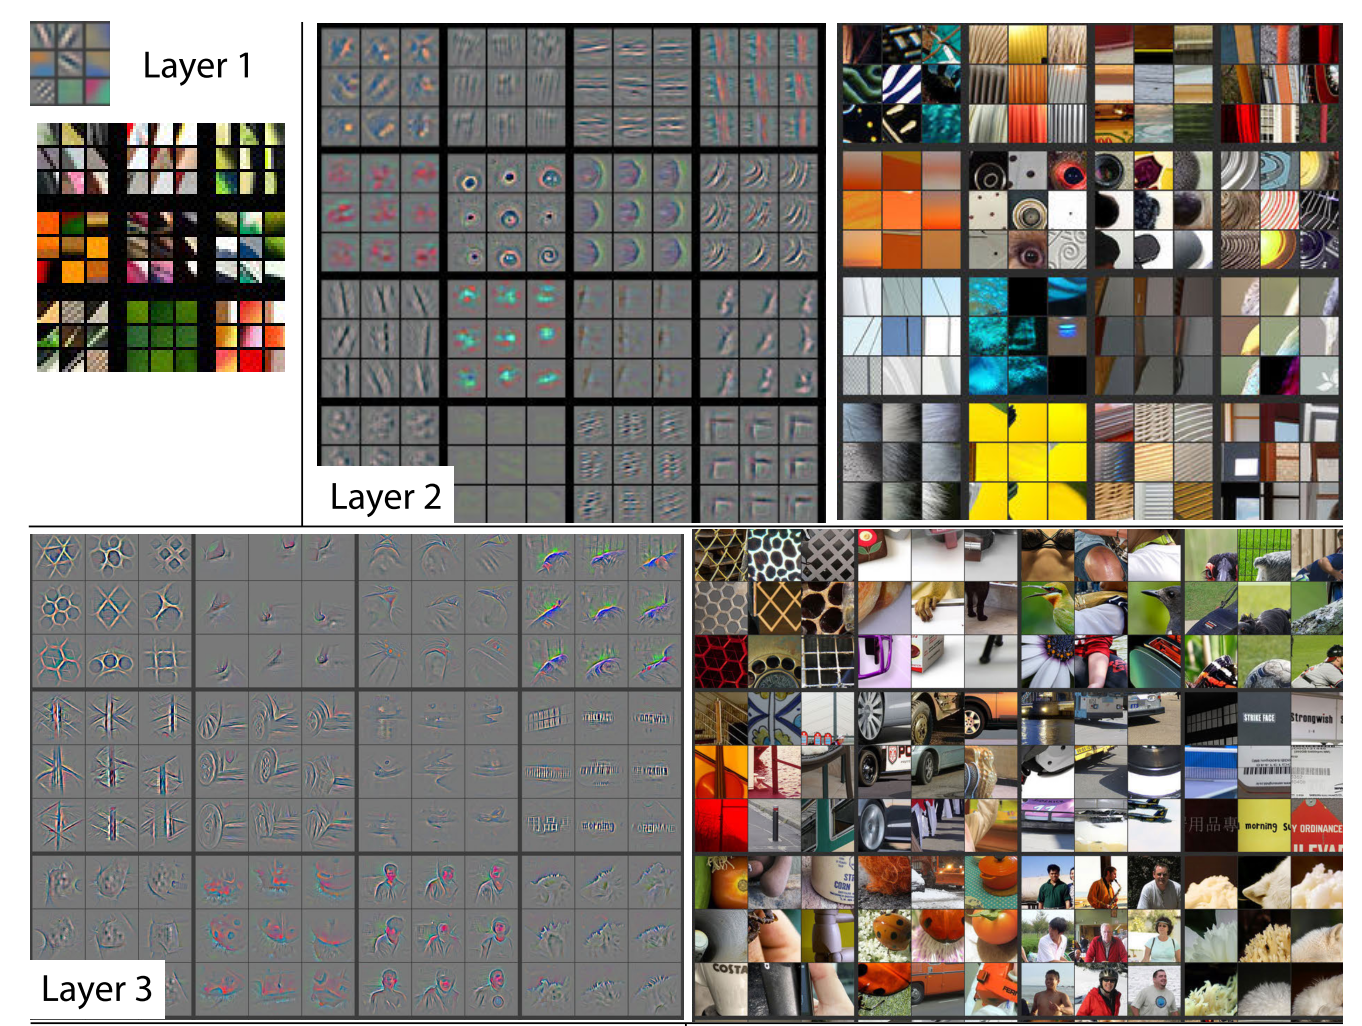
\includegraphics[width=0.5\textwidth]{img/zeiler_deconv.png} 
    			\caption{Zeiler Deconv}%
 		\end{figure}
 		
 		
		\par 
		\textbf{\cite{Erhan2009}} sought to find the optimal stimulation of a unit activations through gradient descent in the image space. This has been criticised as difficult to obtain due to the need for careful initialization, and the lack of information conveyed about a units invariance. 
		\par 
		\textbf{\cite{Le2010}} show how the Hessian of a given node may be computed numerically around an optimal response - thus fixing the formers shortcomings by providing a view of invariances. The issue with this approach is with the higher layers where invariances become increasingly complex and are thus poorly encoded in their quadratic approximations. 
		\par 
		\textbf{\cite{Vondrick2013a}} use feature inversion algorithms, where an image is featurized and then recovered to a transformed but decipherable format - again to give intuitive access to abstract feature representations formed by the network. Using this technique they discovered single deep neurons that were trained to respond to faces and bodies, both human and animal. 
		\par 
		\textbf{\cite{Zeiler2013}} provide a technique called \textit{Deconvolution} \cite{Zeiler2011} which effectively reverses a convolutional network. Deconvolution is a type of feature inversion that renders re-weighted versions of inputs, highlighting areas, patterns and textures of an image deemed most important by a particular part of the network. It essentially approximates a reconstruction of the input of each layer from its output.
		\par 
		Clearly with such a lot of attention placed on visualising featurizations, it's a significant opportunity to learn about the networks. It's important to realise however that one of the above is not necessarily better than the others: each show a different element of the featurisation, and as experts still know relatively little about the behaviour of ANNs it's important to not discard any of these visual aids rashly.
		
\subsection{Evaluation}
While there have been many attempts to visualise the internal processes occurring within neural networks, it is clear that no definitive technique has been discovered. Each technique provides a new tool for the probing toolkit. 
\par 
It is clear however that there is a trend moving away from visualising weights and bias acting on particular neurons towards discovering representation at either a model or layer level. This thesis will attempt to follow that lead.

\clearpage 

\section{Product Goals}
	To help guide the development of a useful visualisation research tool, a small survey of existing researchers was performed. The results of which determined the continual direction for the project.
	\subsection{User Survey \& Interviews}
	\subsubsection{Survey Design}
	\par
	The intial user survey was developed in collaboration with this projects supervisor and was distributed amongst a small number of Imperial College Staff and students known to be working with neural networks. The following areas were addressed.
	\begin{itemize}
	
		\item \textbf{Describe your working environment}
		\par
		This had specific subtopics asking about languages used, packages researchers were familiar with and time taken to develop working networks.
		\item \textbf{Describe your training methods}
		\par
		This asked specifically about how often neural network parameters were adjusted, which of those were considered to be most important, which were the most frustrating changes made and how these challenges were currently solved.
		\item \textbf{Choose which visualisation technique you think is the most useful}
		\par 
		A number of examples from the previous section were shown with weights, gradients, activation mapping, architecture graphing, classification distribution and filters all included. 
		\item \textbf{Choose which element you think would be most useful to visualise}
		\par 
		A list of all the different parameters that could be adjusted during training were given and could be selected.
		\item \textbf{Do you currently visualise neural networks, and if so how?}
		The question asked researchers to mention specific packages that they commonly use and asked about preferred methods for interacting with the software, such as \textit{.csv} upload, model upload, function integration etcetera.
	
	\end{itemize}
	
	\subsubsection{Survey Results}
	\par 
	A relatively small sample was taken, however a second round of delivery was postponed in favour of working on product development and continued research into Neural Networks.
	\par

	\begin{figure}[H]
    			\centering												{{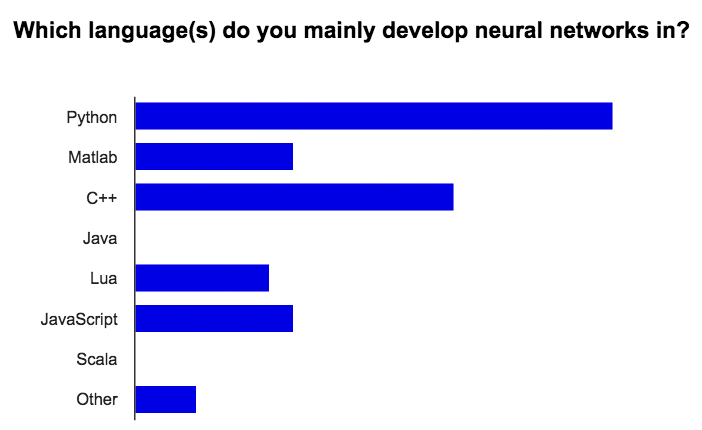
\includegraphics[width=7cm]
    				{img/survey-lang.png} 
    			}}%
	\end{figure}
	
	In response to working environment it was discovered that the majority of participants used python based packages however often single researchers would use multiple different neural network packages depending on the task at hand. For example: CUDA, Caffe, Lasagne, Torch and others. 
	\par 
	
	\begin{figure}[H]
    			\centering												{{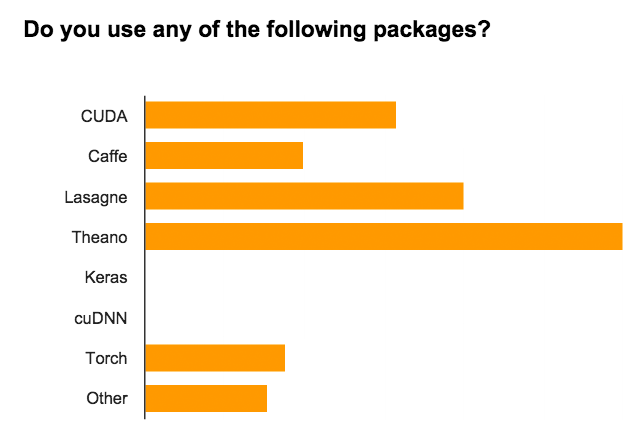
\includegraphics[width=7cm]
    				{img/survey-networks.png} 
    			}}%
	\end{figure}
	
	For some researchers the tweaking of parameters and adjusting of network architectures took up the majority of their time working on PhD's - suggesting tools which aimed to help analyse the success of these changes could be an invaluable addition to their research toolkit. 
	\par 
	In extra comments a wide array of methods were described for deducing the correct network parameters, or judging the quality of one set versus another. One example demonstrating the \textit{`hacky'} nature of tools currently used goes as follows: the researcher would get up on the screen various weight matrices from different training epochs that corresponded to a layer deep within the network and would simply switch tabs as fast as possible to try and observe changing numbers or patterns in the data - signs that the network would be training. While this method appeared to work for this particular researcher, the functionality could certainly be improved by some simple visualisation implementations of the data.
	\par 
	
	\begin{figure}[H]
    			\centering												{{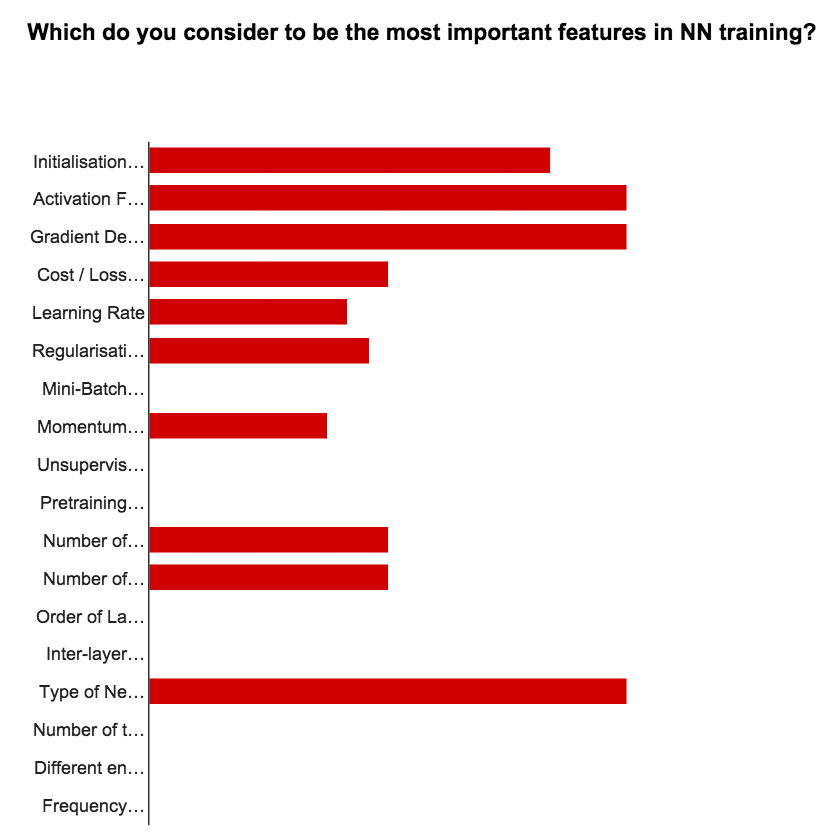
\includegraphics[width=7cm]
    				{img/survey-importance.png} 
    			}}%
	\end{figure}
	
	With respect to commenting on existing visualisations, it was surprising to see that most hadn't thought much about visualisation as a serious tool beyond graphing the commonly used error rates or accuracy. For the majority of time, researchers would simply use visualisation as a way to demonstrate results, not as a research tool.
	\par 
	Importantly, while current usage was limited, researchers generally appeared interested in the possibilities visualisation might hold.

	\subsection{Goals}	
	A number of goals were set after the initial survey and a review of neural networks, visualisation theory \& existing visualisation software.
	\par 
	\begin{itemize}
		\item Improve the visualisation tools currently available for neural network researchers
		\item Provide Visualisations that demonstrate visualisation is actually valuable as a method of research
		\item Visualise changing parts of the neural network: weights / bais matrices, activations etcetera
			 \item Create a visualisation tool that adheres to the visualisation principles set out by Edward Tufte
			\item Investigate not just one visualisation method, but explore a range of options to demonstrate the value of any final product decided upon
			\item Create a tool that is easy for researchers to interact with
			\item Provide a visualisation tool that doubles up as a tool for collecting network data for other data-mining purposes
			\item Keep a full record of experiments taken, and their outcomes
			\item Real time visualisation updates to understand if a currently training network is developing as expected
	\end{itemize}	

\clearpage
\section{Data Collection}
	Visualising neural networks is a complex task. In particular there were three major challenges to address: producing the data, collecting the data and visualising the data.
	\par 
	This chapter will address the first two of these difficulties. In particular this section explores the Neural Network implementations used, the dataset implemented upon and some further considerations made when collecting the data.
	
	\subsection{Neural Network Implementations}
	Often research work pertaining to neural networks requires some new, advanced, model that solves a unique task or demonstrates significant efficiency gains. The purpose here however is quite the opposite. Implementations should be very familiar to those looking into this study. This ensures that a complex network does not obfuscate the true goal of this report - which is to demonstrate the value of a visualisation tool for learning about these networks.
	
	\begin{figure}[H]
    			\centering												{{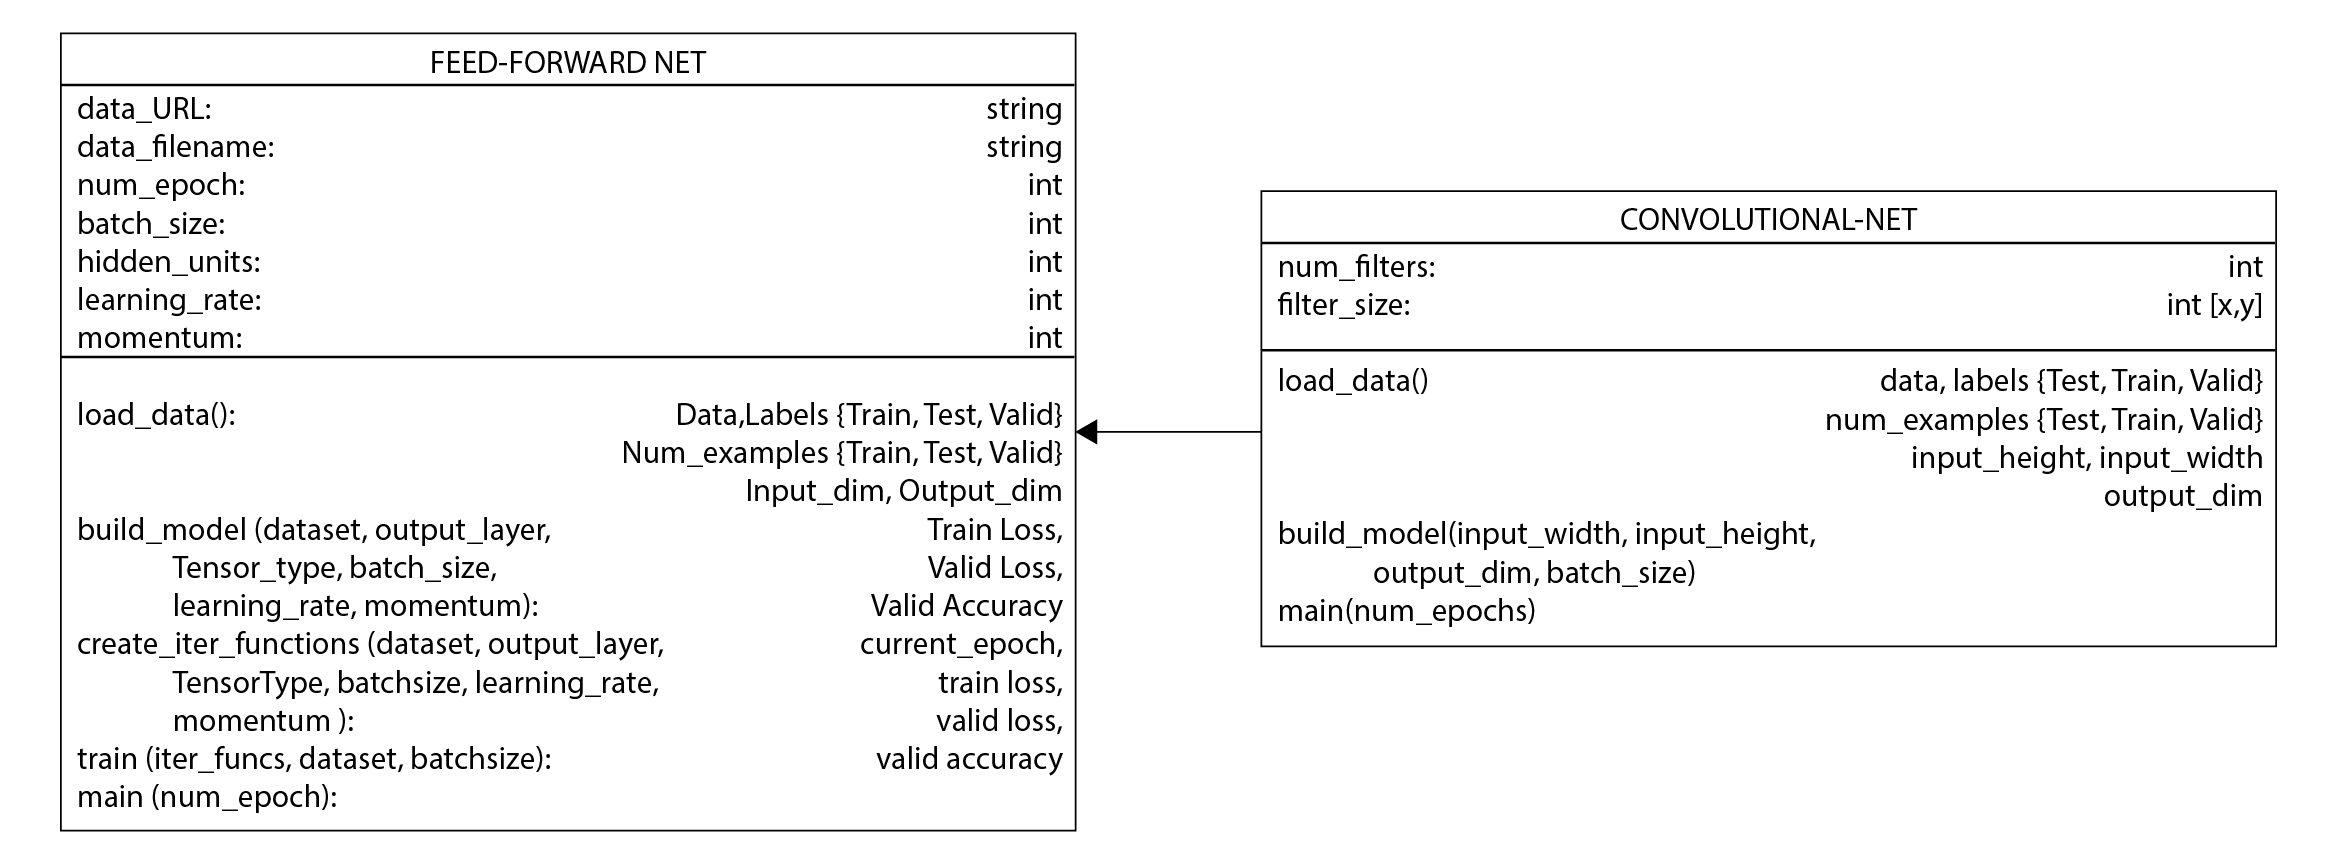
\includegraphics[width=0.7\textwidth]
    				{img/UML_nets.png} 
    			}}%
    			\caption{UML Snippet: Neural Nets}%
	\end{figure}	


		\subsubsection{Feed Forward Net}
		All network models used were adapted from classic architectures. The feed forward network was an implementation of a network proposed in the 2012 Geoffrey Hinton paper in which he explains the concept of drop-out \cite{Hinton2012} - an idea that addresses overfitting,  a significant problem in machine learning. This network is well understood due to the significance of this paper as one of the major recent advancements within the neural network research scene.
	
	\begin{figure}[H]
    			\centering												{{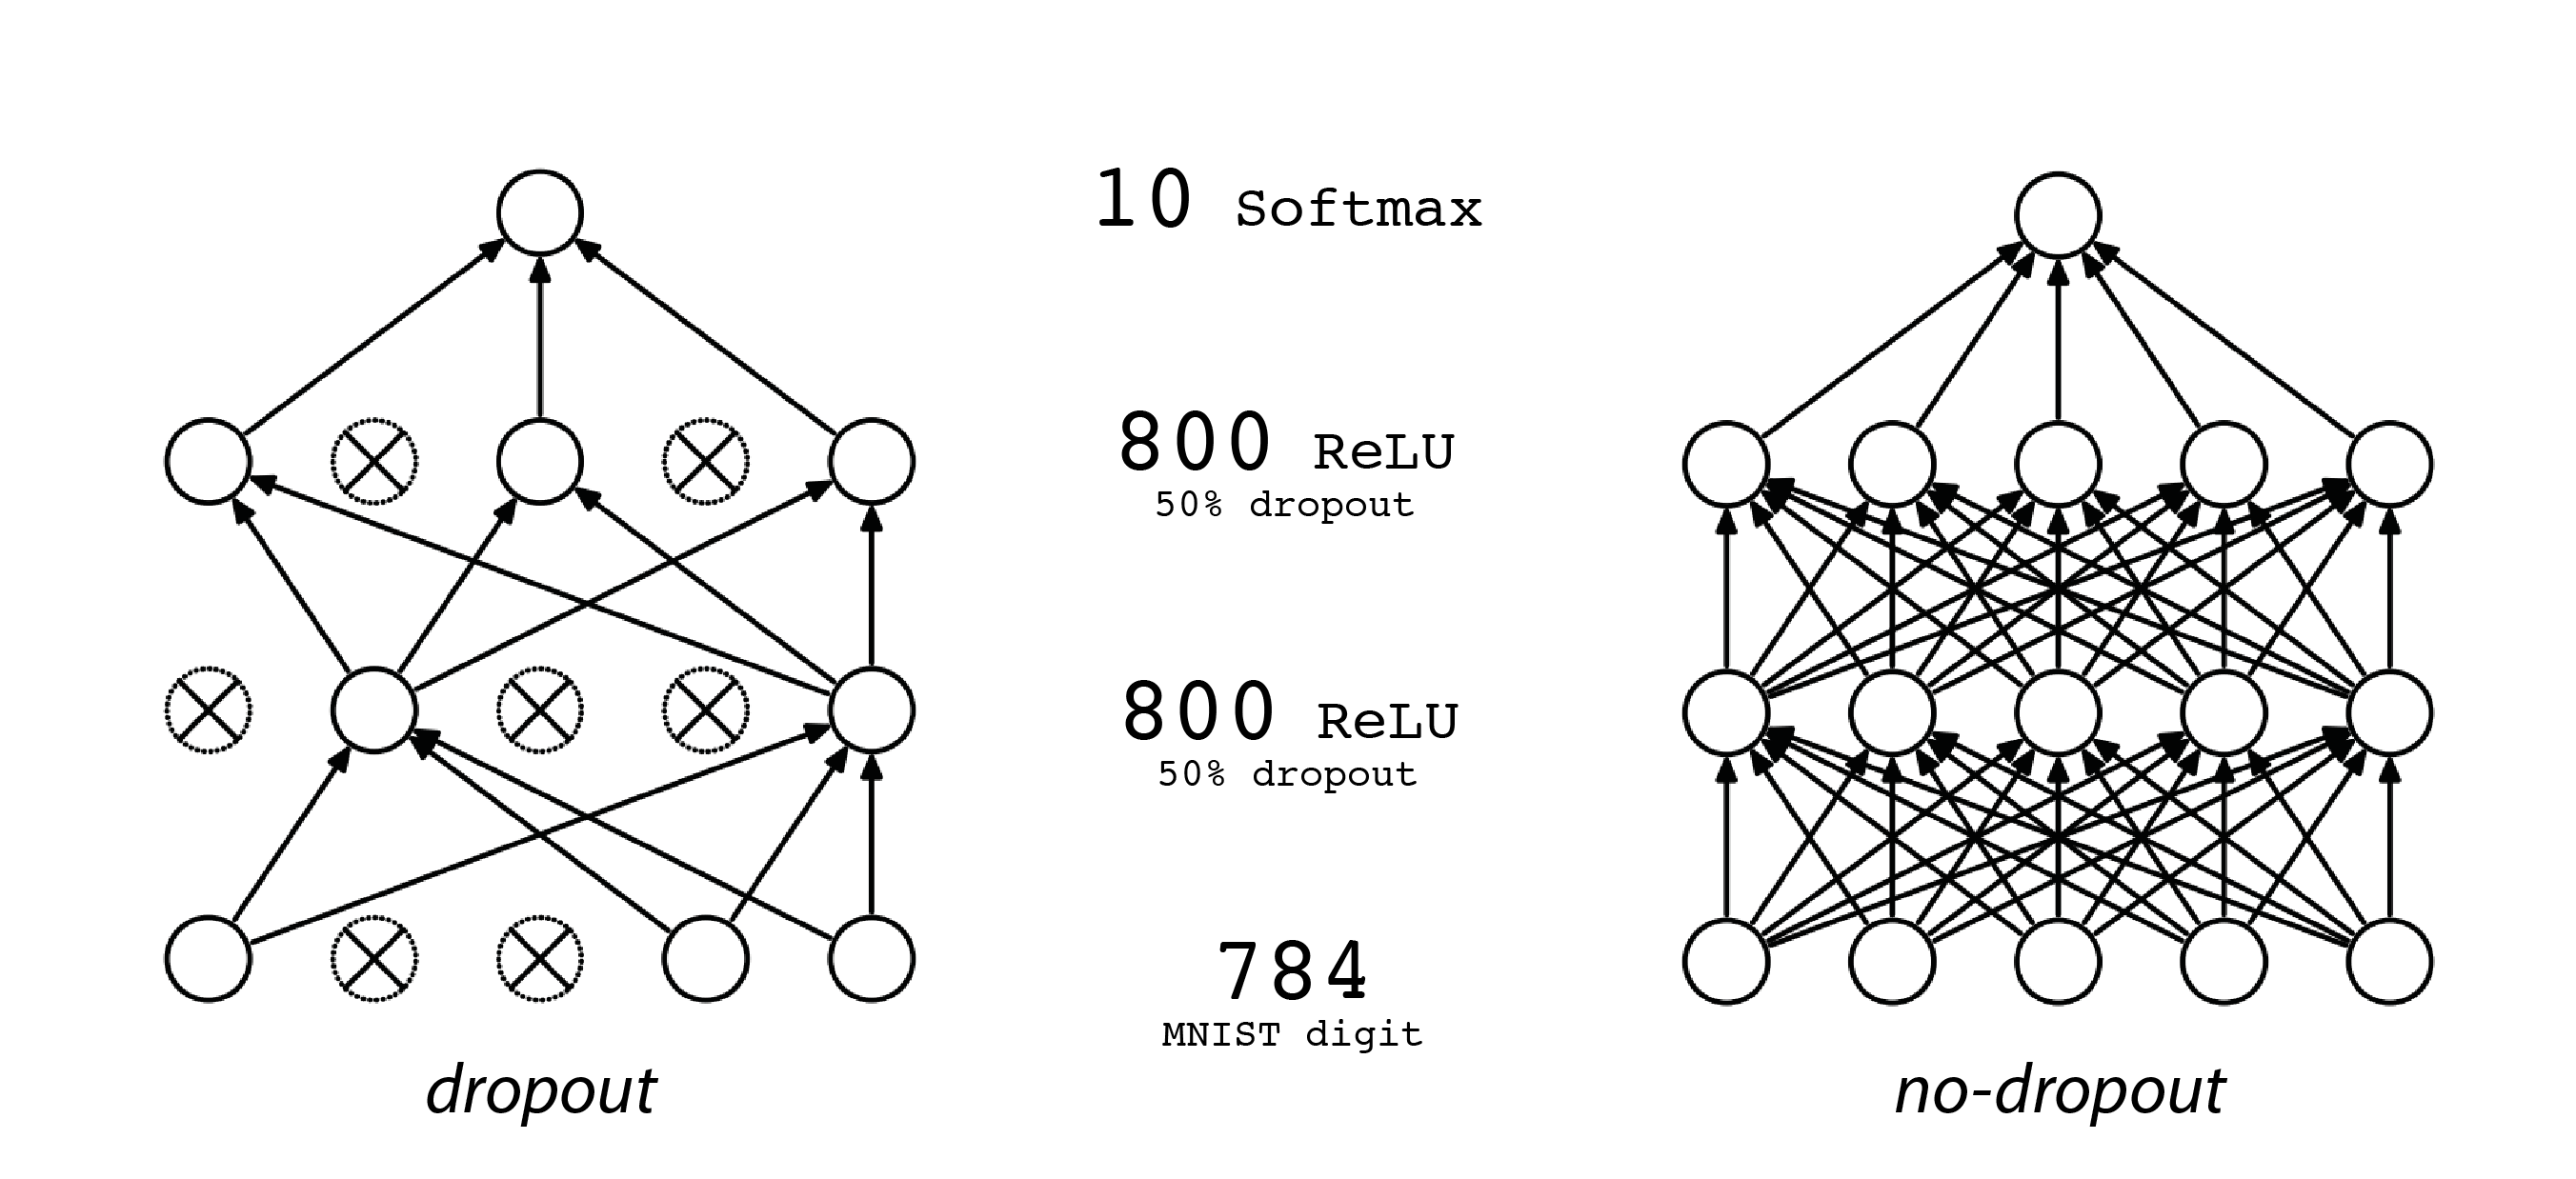
\includegraphics[width=12cm]
    				{img/hinton_dropout_2012.png} 
    			}}%
	\end{figure}

		\par 
		The network itself takes 784-input values - the (28,28) MNIST images flattened into a single array - followed by two layers of 800 ReLU units and an output Softmax layer of 10 units - digits zero to nine. 
		\par 
		Other parameters used from the Hinton paper include a 50\% drop-out rate between hidden layers and 100-sized mini-batches. The implementation in this project differend in the number of epochs the experiments were run for. This was a trade off that enabled more visualisation tests to be performed, and is afforded by the minimal need to prove an accurate model, which has already been demonstrated.
		\\\
		\subsubsection{Convolutional Net}

		The convolutional architecture used throughout the project is a common adaptation of Yann LeCun's 1998 LeNet \cite{LeCun1998}, the first network to successfully classify handwritten digits: 
		\begin{itemize}
			\item Layer Input: (60000 [size of training set], 1, 28, 28 [dimensions of MNIST image])
			\item Layer 1: Convolutional Layer: 32 Filters, (3,3) Filter Size, (2,2) Pooling
			\item Layer 2: Convolutional Layer: 64 Filters, (2,2) Filter Size, (2,2) Pooling
			\item Layer 3: ReLU layer: 500 Units, 50% dropout
			\item Output: Softmax: 10 Units
		\end{itemize}
		\par 
		
		\subsubsection{Alteration}
		The above implementations are know to produce desirable results which gives a test subject baseline, however they are altered in a number of ways throughout this project. 
		\par 
		In order to explore the ability of visualisation methods to capture interesting and important patterns within a networks output data such that it can influence researchers decisions, the network must be \textit{broken} across a number of different parameter settings.
		\par 
Using a variety of different parameter settings, it is possible to simulate the changes that a researcher might make when exploring the parameter space for optimal performance.
		
	\begin{figure}[H]
    			\centering												{{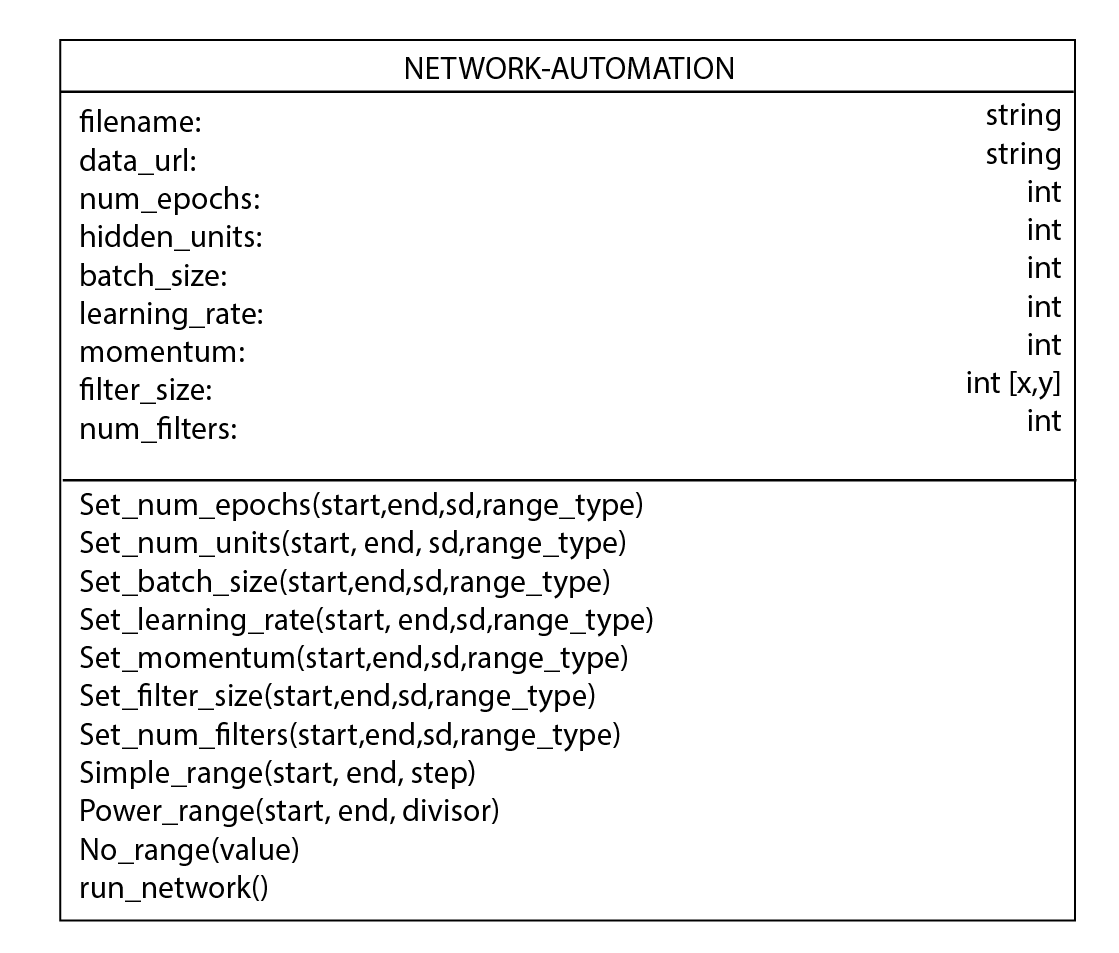
\includegraphics[width=0.5\textwidth]
    				{img/UML_auto.png} 
    			}}%
    			\caption{UML Snippet: Automatic Networks}%
	\end{figure}	
	
		\par 
		To successfully implement these changes, a power range was defined that would run fewer experiments as it neared the understood value - \textit{[1, 2, 3, 5, 7, 11, 17, 25, 38, 57, 86, 129, 194, 291, 437, 656]} - these values are examples run for the number of hidden units used within the networks. However other parameters were automatically tweaked including number of epochs, learning rate and momentum. Other parameters which required tweaking in the neural network code base itself were less scientifically adjusted - such as the number of hidden layers, or type of non-linearity used.
		
		\subsubsection{Practical Implementation}
		The neural networks described above were implemented in \textit{Lasagne}, a library designed for building neural networks.
		\par 
		Lasagne is a neural network wrapper for the common machine learning python library \textit{Theano} which uses symbolic functions that compile before runtime into \textit{cython} to ensure efficient mathematical processing, often displaying efficiency gains of up to 10 times.
		\par 
		Lasagne was chosen as the network implementation package after the survey of participants revealed that the largest minority of researchers currently used Python implementations of neural networks. Theano could have also been used, however was deemed overly complex for the purposes of this project. 
		\par 
		It's important to note that in this incredibly fast moving field that the frontrunning technology is continually changing and throughout the course of this project another library \textit{Torch} has become increasingly popular due largely to it's ability to handle \textit{Recurrent Neural Networks}. These haven't been mentioned in this report for simplicity reasons. 
	
	\subsection{Dataset}

	All experiments for this project were conducted using the MNIST dataset. The dataset is widely used as a  benchmarking dataset not just within the neural network community but in the wider machine learning community as a whole, making it appropriate as a test dataset. The dataset itself contains 60,000 training images and 10,000 test images. Each image is a 28 pixels by 28 pixels hand-written digit from one to nine.
	
	\begin{figure}[H]
    			\centering												{{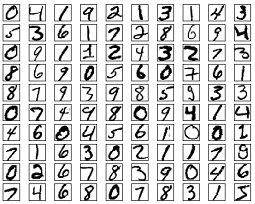
\includegraphics[width=7cm]
    				{img/mnist_digits.png} 
    			}}%
    			\caption{100 MNIST digits}%
	\end{figure}
	

	\par 
	The CIFAR datasets could have also been used however MNIST was chosen due to its representation being confined to one set of intensity values, rather than the more complex CIFAR set with Red, Green and Blue dimensions to consider. The below images demonstrate the simplicity of the dataset.

	\begin{figure}[H]
    			\centering	
    			\subfloat[MNIST digit]								{{
\includegraphics[width=0.2\textwidth]
    				{img/mnist_four_image.png} 
    			}}%
    			\qquad
    			\subfloat[Intensities]																			{{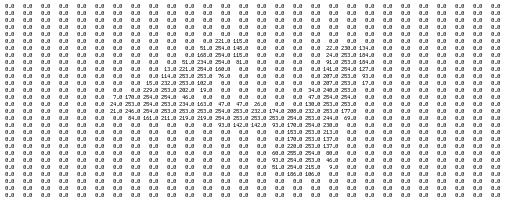
\includegraphics[width=0.5\textwidth]
    				{img/mnist_four_intensities.png} 
    			}}%
    			\caption{}%
    			\label{fig:mnist_four}
		\end{figure}

\subsection{Collecting Output Data}
	There was a lot of data handling within this project, a few considerations about this are described below.
	\begin{itemize}
		\item Data used online was stored in a compact format. This was achieved using a MongoDB database to store \textit{JSON} objects in binary - \textit{BSON}. In earlier iterations of the project this was interfaced with using a JavaScript backend, and in the later iteration of the project using the python library \textit{PyMongo}.
		\item Data that researchers use to assess the quality of their models was also stored and in a common format that can be easily interrogated. This was achieved by using Python's sophisticated \texttt{sys} and \texttt{os} packages to store the weights, biases, activations and other parameters in \textit{csv} format.
		\item Data from the neural networks must retain its shape for easy importing with the python library \textit{numpy}. This was achieved by either using numpy to process the data, or by creating bespoke input-output functions that would deconstruct and reconstruct the data's shape.
		\item Image data was be transformed in order to be processed with MongoDB. This is achieved by preprocessing the data with the python library \texttt{base64} which parses the images into a Float32 array in base64 notation - this then usefully becomes small enough to store in the \textit{MongoDB} document.
		\item Coordinate data for scatter plots was stored in a condensed format that enables easy interaction with the \textit{d3.js} visualisations. Here, (500, 2) matrices are \texttt{numpy.reshaped} to (1000,) single dimension arrays which can be easily parsed by the d3.js client configuration.
		\item Activation data was temporarily stored before being converted into scatter plot x-y data by the tSNE algorithm.
	\end{itemize}
		
	\begin{figure}[H]
    			\centering												{{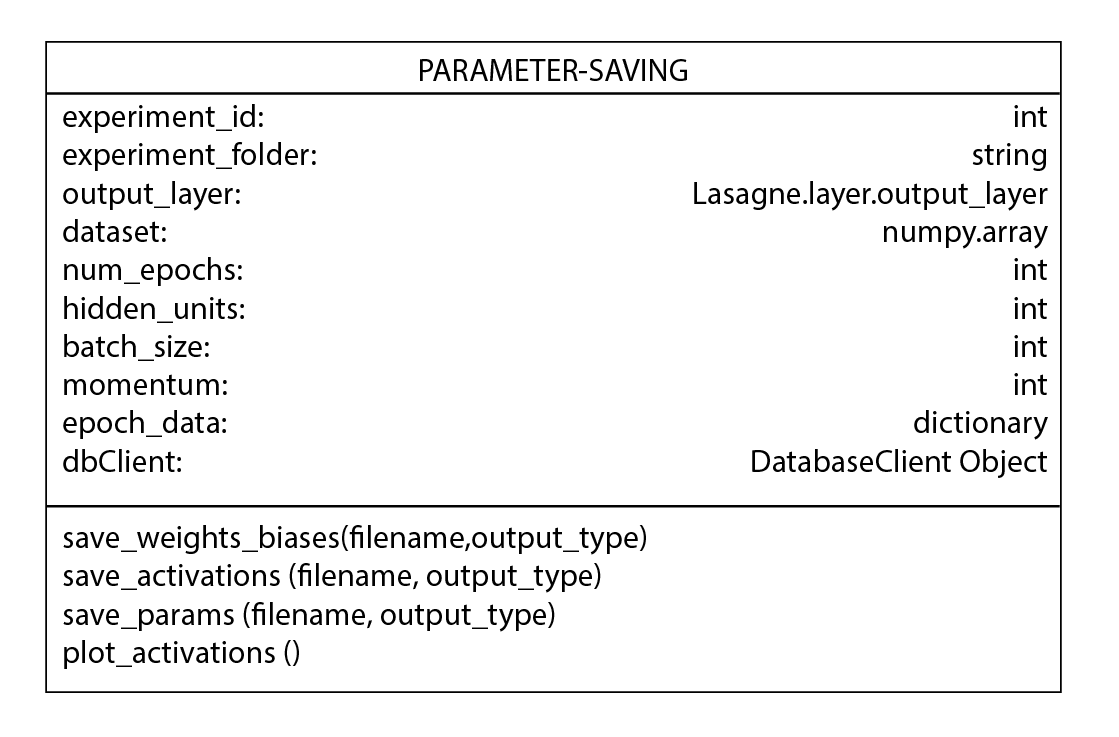
\includegraphics[width=7cm]
    				{img/UML_saving.png} 
    			}}%
    			\caption{UML Snippet: Saving Functionality}%
	\end{figure}		
	
	The data collection methods described above interact with the complex machinery of a neural network. To effectively store the relevant data, it was important to fully understand how the discrete pieces of information interacted with one another. The following entity relationship diagram describes the majority of the features that this concerned.

	\begin{figure}[H]
    			\centering												{{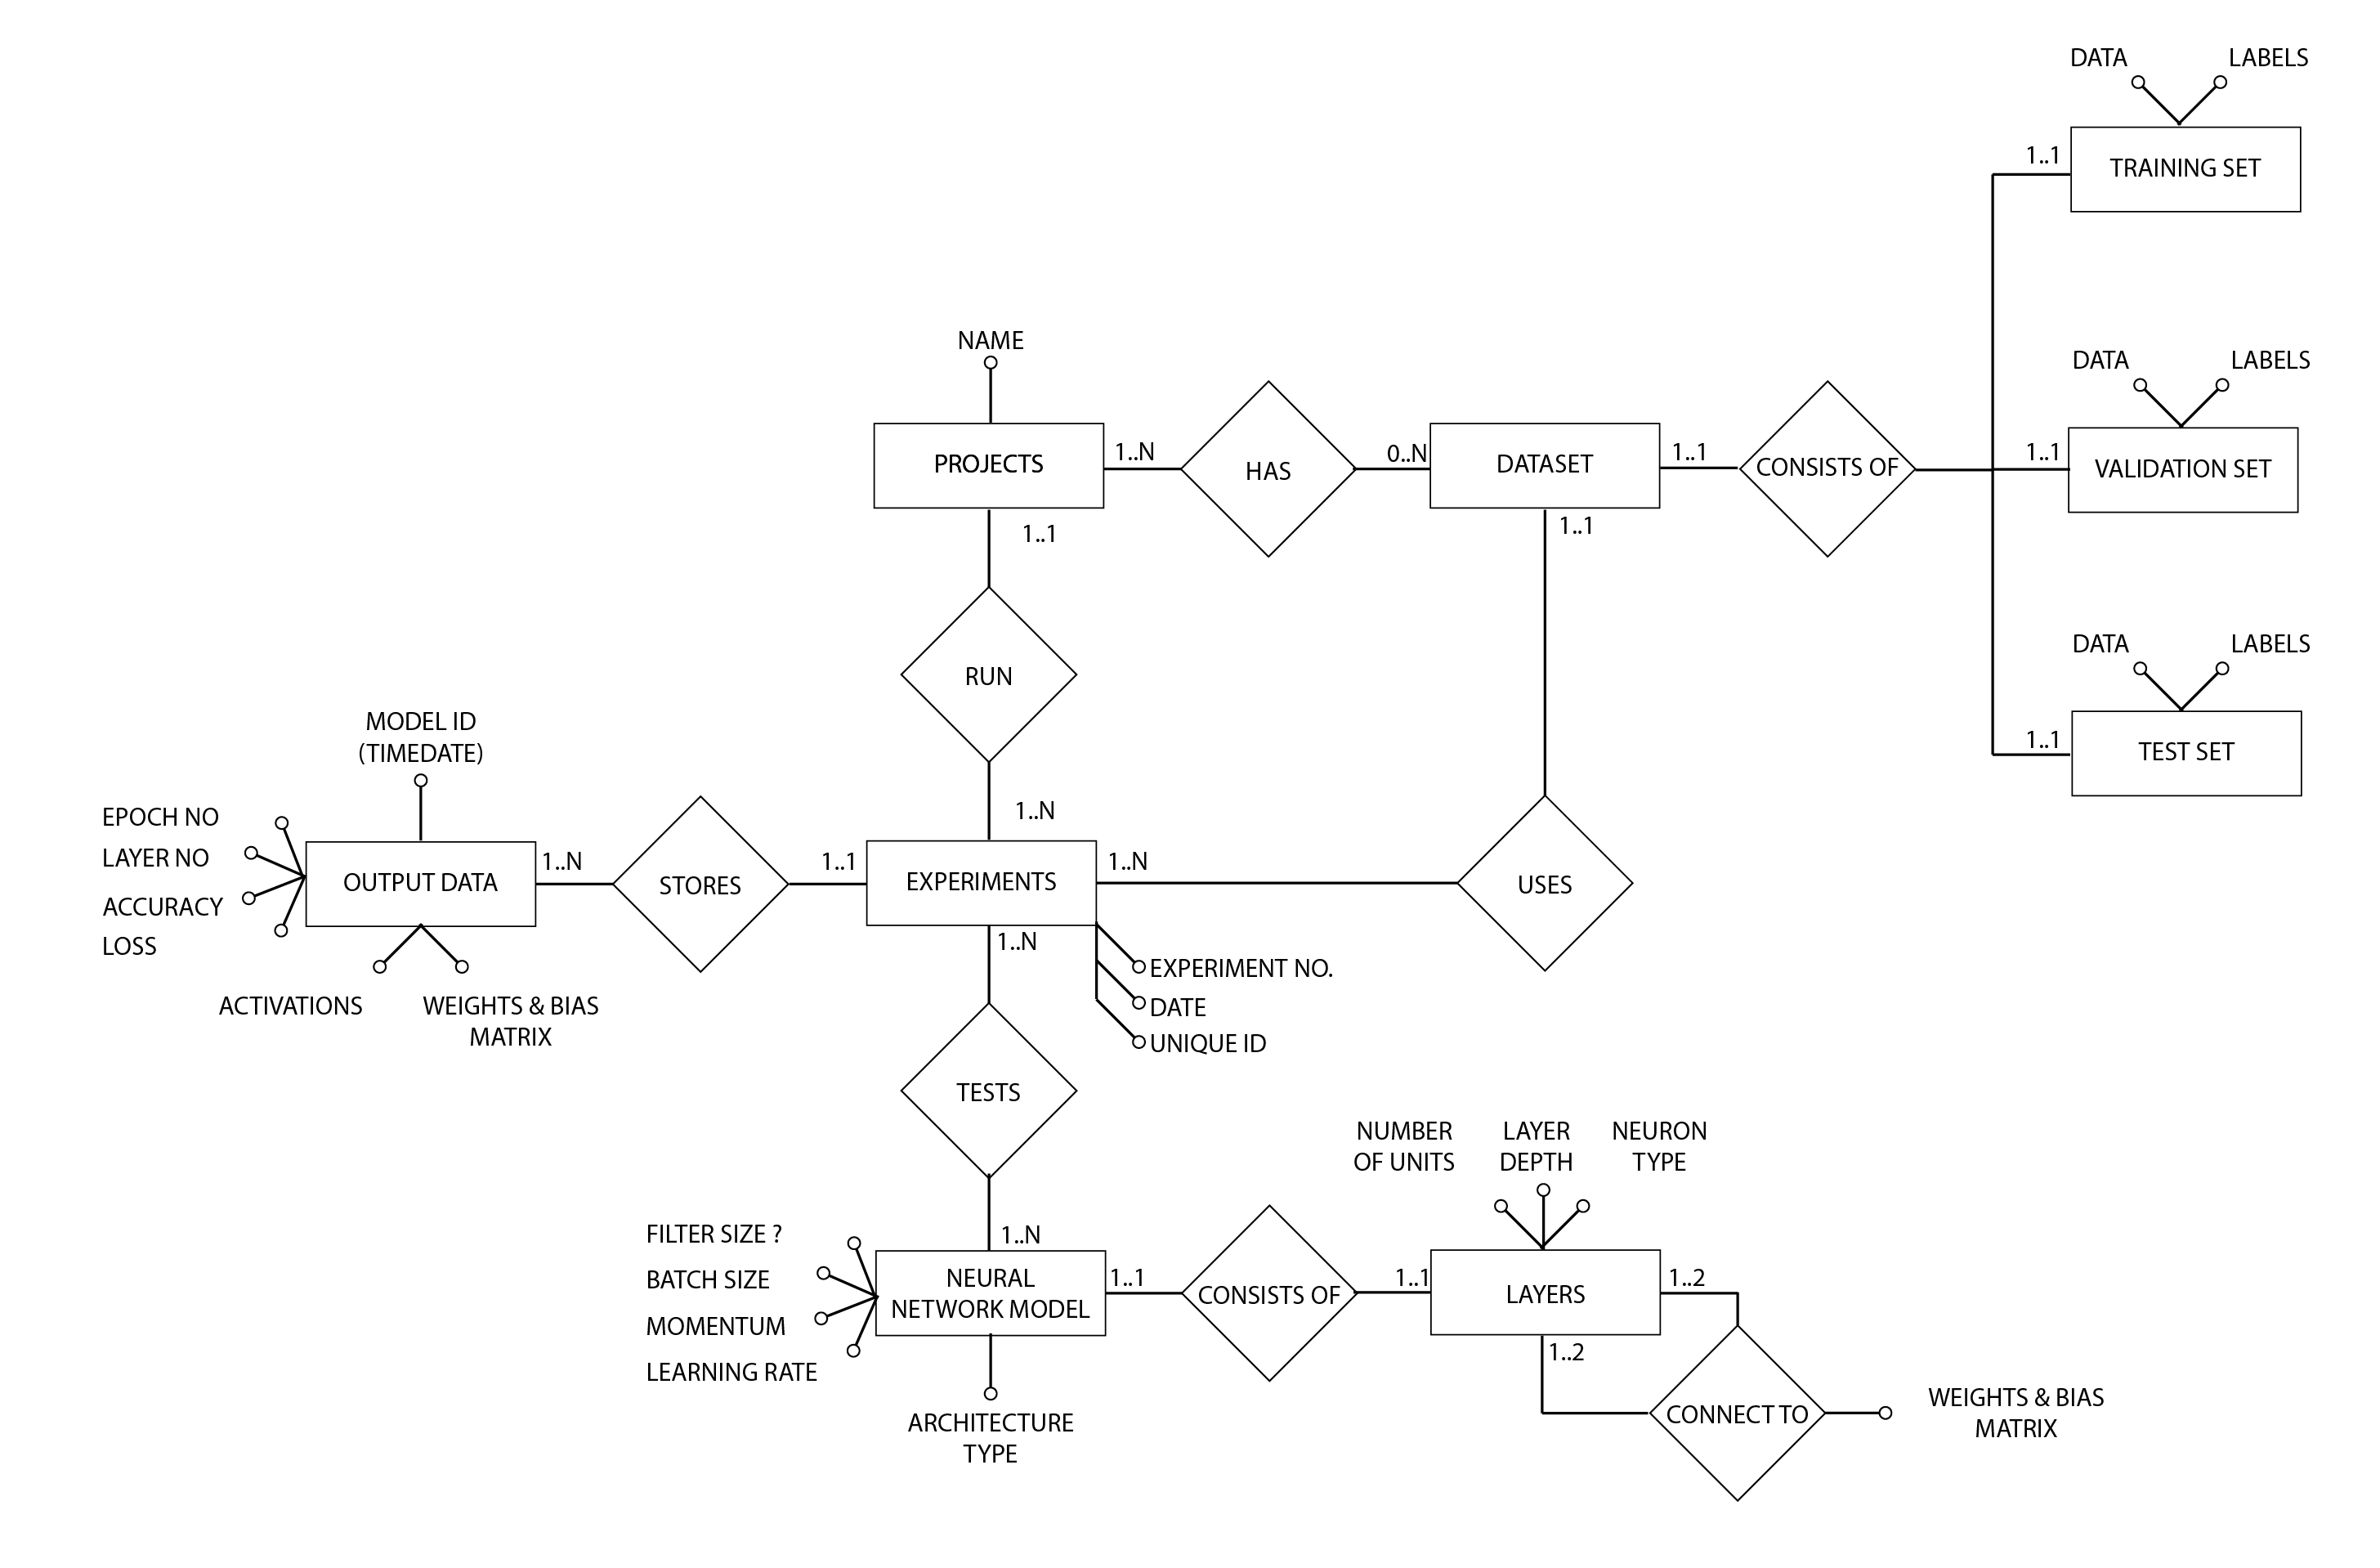
\includegraphics[width=17cm]
    				{img/ER_horiz.png} 
    			}}%
    			\caption{Initial ER diagram}%
	\end{figure}	
	
\subsection{Evaluation}
The aim of this first section was to explain to the reader the foundation upon which this project was built. Namely, two well understood neural networks that get modified in various ways away from understood parameters that ensure optimal performance. This is done to better understand how poor networks may appear when visualised, and to observe differences between those and the networks known to be of industry standard. The section also explains the importance of gathering the data outputs of these networks in an appropriate fashion, and the reasons for choosing the MNIST dataset. 
	\par 
	With a basic understanding of the neural networks and dataset used, and an understanding of the data collection methods, the remainder of the report will explore how this data can now be visualised.

\clearpage
	
\section{Dimensionality Reduction}

Neural Networks are famous for their ability to comprehend complex datasets such as in areas of vision or speech recognition. One of the principle complications in these fields results from complex high-dimensional datasets.

 	\begin{figure}[H]
    			\centering	
			{{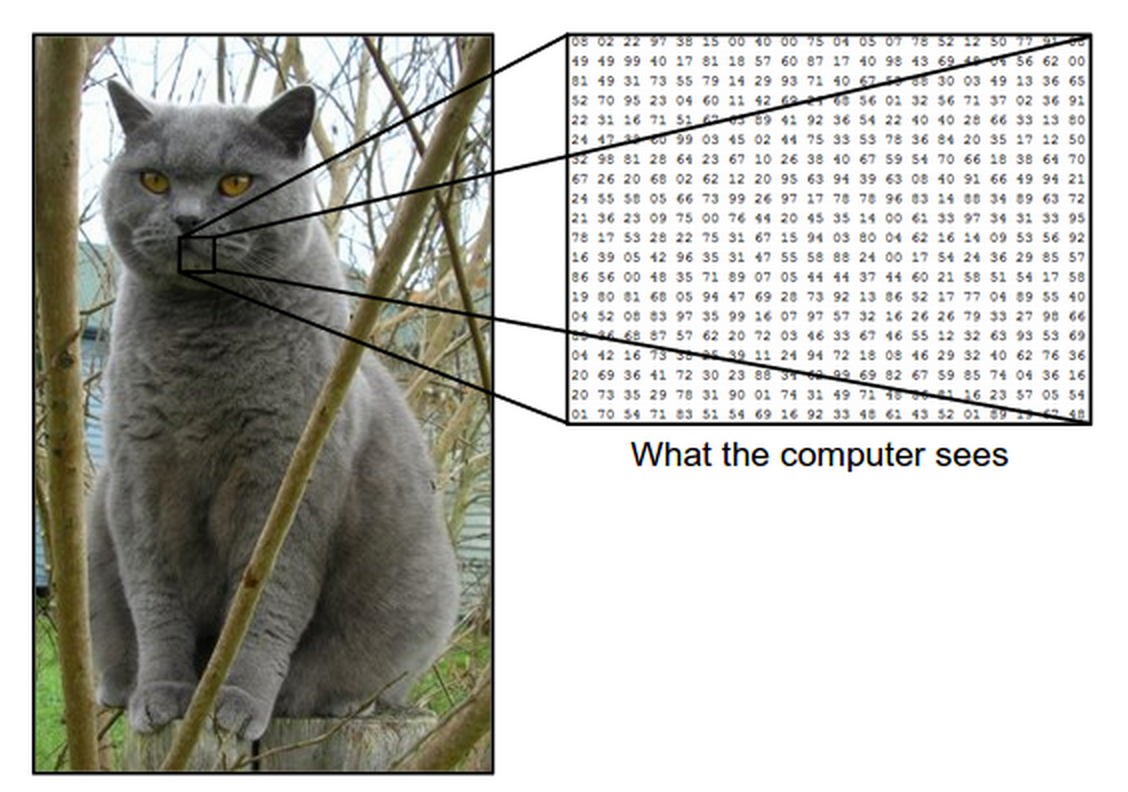
\includegraphics[width=0.45\textwidth]
    				{img/catimage.png} 
    			}}%
    			\caption{Cat}%
    		\label{fig:lascaux}
	\end{figure}
	
	The image above is 248 pixels wide, 400 pixels tall, and has three colour channels Red, Green and Blue - which to the computer is stored in a multidimensional array of dimensions (248,400,3) or 297,600 numbers. When this image is passed into the computer it understands this data as 297,600 different data points - not as a cat.
	\par 
	As this image passes through a neural network, the number of dimensions (248,400,3) changes to make it easier for the network to classify as a cat - one of 10 classes in the CIFAR-10 dataset. So while a human can understand this image as a cat, when the data is transformed to (512,20,2) dimensions the cat is no longer recognisable - but to a computer, may be more `cat-like'.
	\par 
	It has been suggested that one reason for the success of neural networks is that they discover optimal representations of the data that allow for more accurate classification \cite{Hinton1986}. These representations are captured in the later layers transformed data-space.
	\par 
	For an example of this take two curves: while at the input space of the network a relatively complex line is required to divide two curves on the plane, each new layer transforms the spatial data creating a new representation that is easier to classify with a more simple hyperplane.
				
		\begin{figure}[H]
    			\centering	
    			\subfloat[No hidden layer]							{{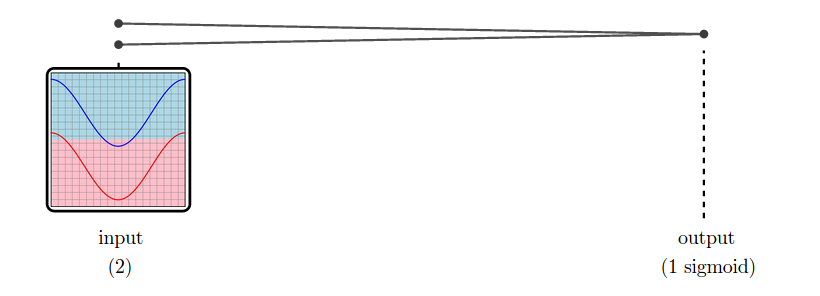
\includegraphics[width=7cm]
    				{img/colah_nonwarp.png} 
    			}}%
    			\qquad
    			\subfloat[Hidden Layer - easier to separate]
    			{{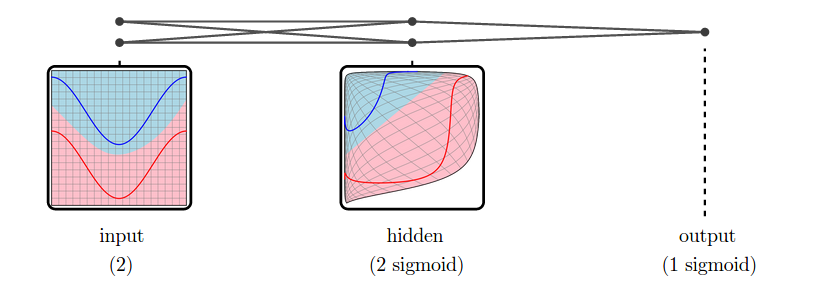
\includegraphics[width=7cm]
    				{img/colah_warp.png} 
    			}}%
    			\caption{Chris Olah: Representations that warp the data}%
		\end{figure}		
		
		\par 
		In order for the data to be transformed to this new representation, it must undergo a sequence of manipulations. A tanh layer for example processing the function $ tanh(Wx + B) $ consists of; 
		\begin{itemize}
			\item a linear transformation by the weight matrix $ \bm{W} $
			\item a translation by the bias vector $ \bm{b} $
			\item and a point-wise application of the tanh activation function
		\end{itemize}
		Intuitively, what is occurring here is a stretching and warping of the space to make it easier to linearly divide - as can be seen above. Note that it does not cut, break or fold the space as it must retain it's `topological' properties \cite{Choi2005}.
	\par 
 	Visualising the information contributing to these representations - the weight matrix, the bias vector and the activations - in a way that is understandable to the human brain, and therefore useful as a diagnostic tool, requires mapping the vast number of dimensions present to the three spatial dimensions that  humans understand with ease. 
	\par 
	This section will explore both visualising high-dimensional data, where the aim is to retain data fidelity and show all of these high dimensional data points, and the notion of dimensionality reduction - where the aim is to instead reduce the number of dimensions mathematically.

\subsection{Visualising High-Dimensional Data}
	Visualising high-dimensional data is a very important problem in several different domains and is a very well explored problem. A number of techniques for visualising high-dimensional data exist, a summary of which was composed by \cite{Cristina2003}.
	\par 
	This covers techniques by a number of different authors that could be useful for the visualising of neural network data;	
		\par
		
 	\begin{figure}[H]
    			\centering	
			{{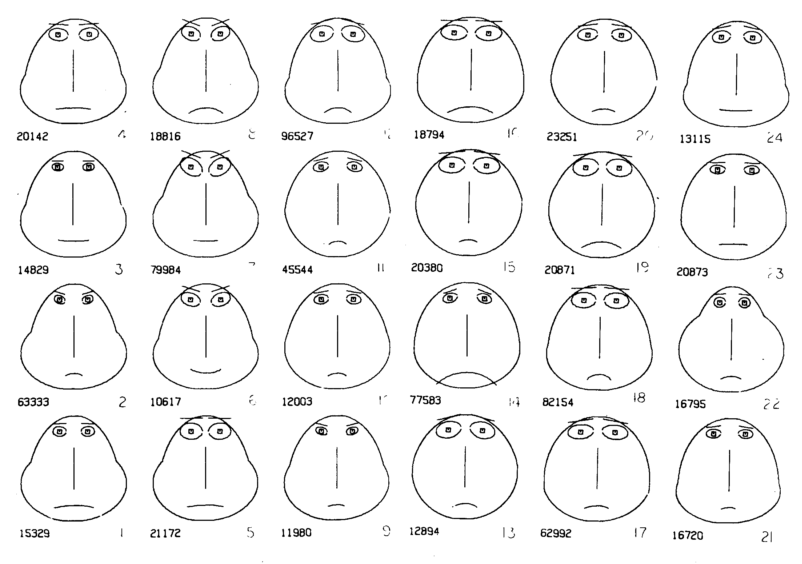
\includegraphics[width=0.3\textwidth]
    				{img/chernoff_faces} 
    			}}%
    			\caption{Chernoff Faces}%
    		\label{fig:lascaux}
	\end{figure}
 		
		 \textit{Chernoff Faces} are iconographic visualisations of faces by \cite{Chernoff1973}; each point in k-dimensional space, $ k < 18 $, is represented by a cartoon of a face whose features, such as length of nose and curvature of mouth, correspond to points in the data. Thus every multivariate observation is visualized as a computer-drawn face. Looking at the recognisable faces it's easy to see which data points are similar and which parameters they share in common. For example, those faces with larger eyes could represent similarities across a gender dimension. This technique is not useful for most neural networks however which have greater that 18 dimensions, but could be compared with some of the low-fi visualisations explored earlier.
		 \par
 		
 	\begin{figure}[H]
    			\centering	
			{{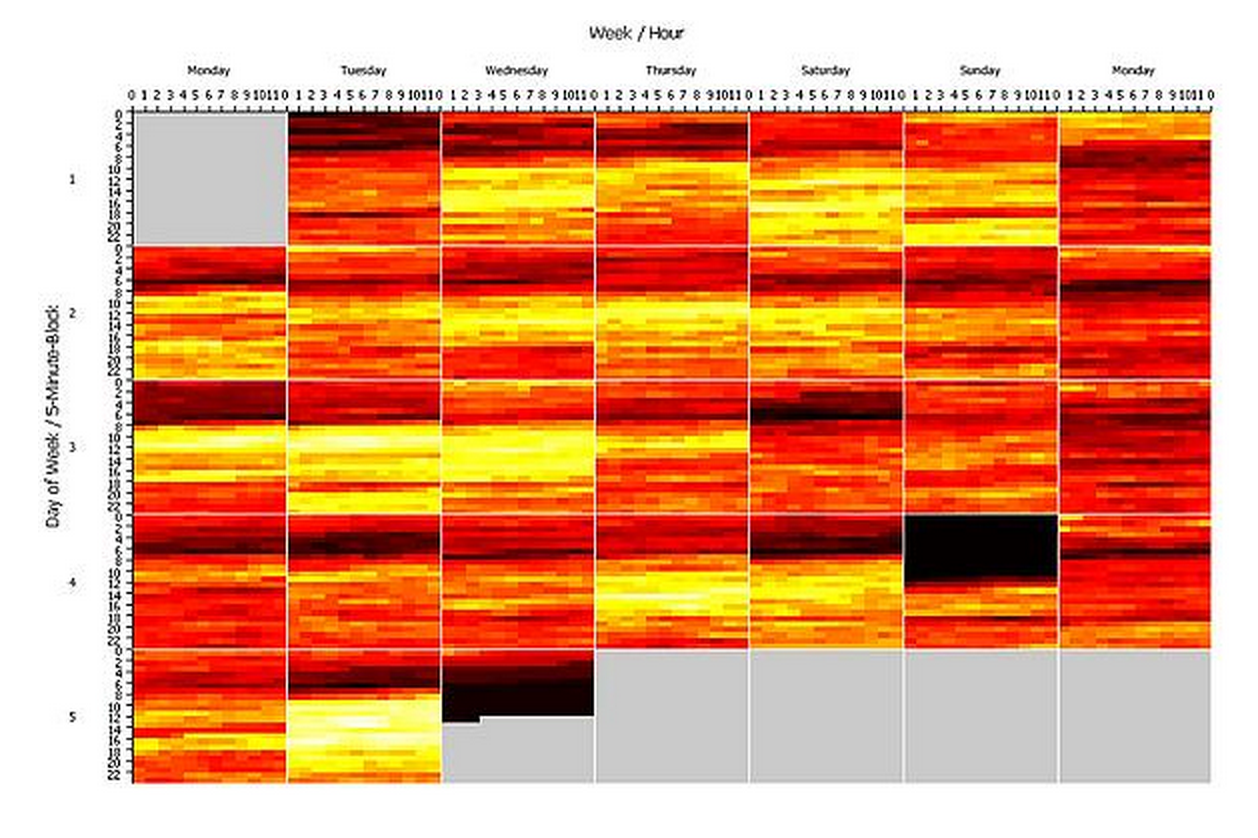
\includegraphics[width=0.3\textwidth]
    				{img/kiem_pixel_two} 
    			}}%
    			\caption{Pixel Based Techniques}%
    		\label{fig:lascaux}
	\end{figure}	
 		
		\textit{Pixel Based}; represent as many data points as possible on the screen at the same time by mapping each data value to a pixel on the screen and rearranging those pixels to suit the source \cite{Keim2000}. One example is to use a gradient of colour to represent the value of a data-point, and multiple dimensions may be show in different as slices tiled together.
		\par 
		 		
	\begin{figure}[H]
    			\centering	
			{{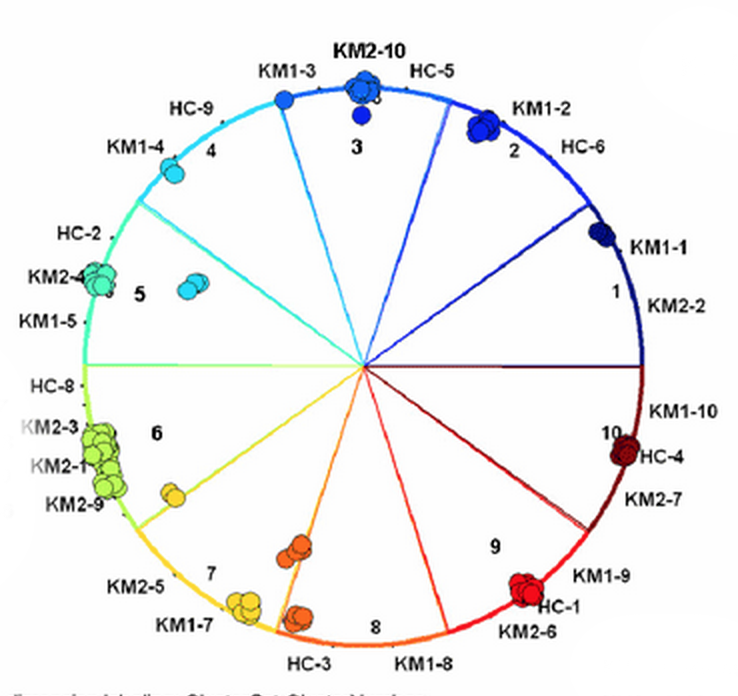
\includegraphics[width=0.3\textwidth]
    				{img/battista_vertices} 
    			}}%
    			\caption{RadViz}%
    		\label{fig:lascaux}
	\end{figure}	 		
 		
 		
		\textit{Radial Coordinate Visualisation} was designed by\cite{Hoffman1999}; which for an n-dimensional visualisation, n lines emanate radially from the center of a circle and terminate at its perimeter; here each line is associated with one attribute. The points that sit in amongst the radial portions represent the data described between the dimensions in a way that is similar to an x-y plot.
		\\\
		\\\
	\textbf{Evaluation}
	\par 
	While these tools do have their uses as visualisation techniques, when it comes to exploring the high-dimensional data of neural networks they have been criticized \cite{Maaten2008} as simply providing the tools to \textit{display} more than two data dimensions, and leave the more difficult task of interpretation to the viewer. With the number of dimensions used in real-world neural networks often in the thousands, these techniques may provide limited insight, and so it's important also to look at dimensionality reduction which performs some of the data interpretation for us.
\\\

\subsection{Dimensionality Reduction}
	Dimensionality reduction differs from the visualisation of high-dimensional data by instead converting the high-dimensional data set  $ X = \{ x_{1}, x_{2},..., x_{n} \} $ into a low-dimensional data set $ X = \{ x_{1}, x_{2} \} $ that can then be displayed easily in a standard recognisable formats such as the scatter plot. Dimensionality reduction aims to preserve as much of the significant structure of the data in higher-dimensions as possible while generating a low-dimensional representation that is easier for the researcher to interpret. This is fundamentally important for visualising neural nets where activations are often many thousands of dimensions.
		\par 
		These algorithms work by drawing a notion of how successful this dimensional reduction is by assuming that for any two data points, $ x_{i} $ and $ x_{j} $ there are two notions of distance between them that can be compared. First, is the distance between those points in the real world space, for example the L2 distance $ d(x_{i,j}) = \sqrt{\sum\nolimits_{n} (x_{i,n} - x_{j,n})^2 } $, and the other is the  distance between the points in the visualisation, $ d_{viz}(x_{i,j}) $, such that a cost function of the visualisations success can be defined.
		\par  		
		If the cost $ C $ is high, then the distances are dissimilar to the original space, if low they are similar, and if zero the visualisation is a perfect representation. It's almost impossible however to get a perfect representation in all aspects, so different cost functions provide different compromises and insights. Once the cost function is designed there simply exists an optimisation problem that can be tackled though a standard process such as gradient descent to ensure that points are optimally visualised with respect to the cost function. The cost function for standard Multi-dimensional Scaling \cite{Torgerson1952} is shown below: 
		$$
			C = 
			\sum\limits_{i \neq j}
			[d(x_{i,j}) - d_{viz}(x_{i,j}) ]^2
		$$
		\par 
		Another reduction method is Sammon's mapping \cite{Sammon1969}, which aims harder to preserve the distances between nearby points than those further away. If the two points are twice as close in the original space than  two others, it is twice as important to maintain the distance between them. This emphasises the local structure at the compromise of the global structure in the data:
		$$
			C = 
			\sum\limits_{i \neq j}
			\frac{ [d(x_{i,j}) - d_{viz}(x_{i,j}) ]^2 }					{d(x_{i,j})}
		$$
		A number of other techniques were reviewed by \cite{VanderMaaten2009} describing \textit{Principle Components Analysis, PCA,} \cite{Hotelling33} - which finds the angle that spreads out the points the most in order to capture the largest variance possible, and \textit{Multidimensional Scaling} as seen above - as linear techniques that keep low-dimensional depictions of dissimilar points far away, but which fail to keep those data-points which are similar close together in the lower dimensional depiction placing an emphasis on global structure.
 		
 	\begin{figure}[H]
    			\centering	
			{{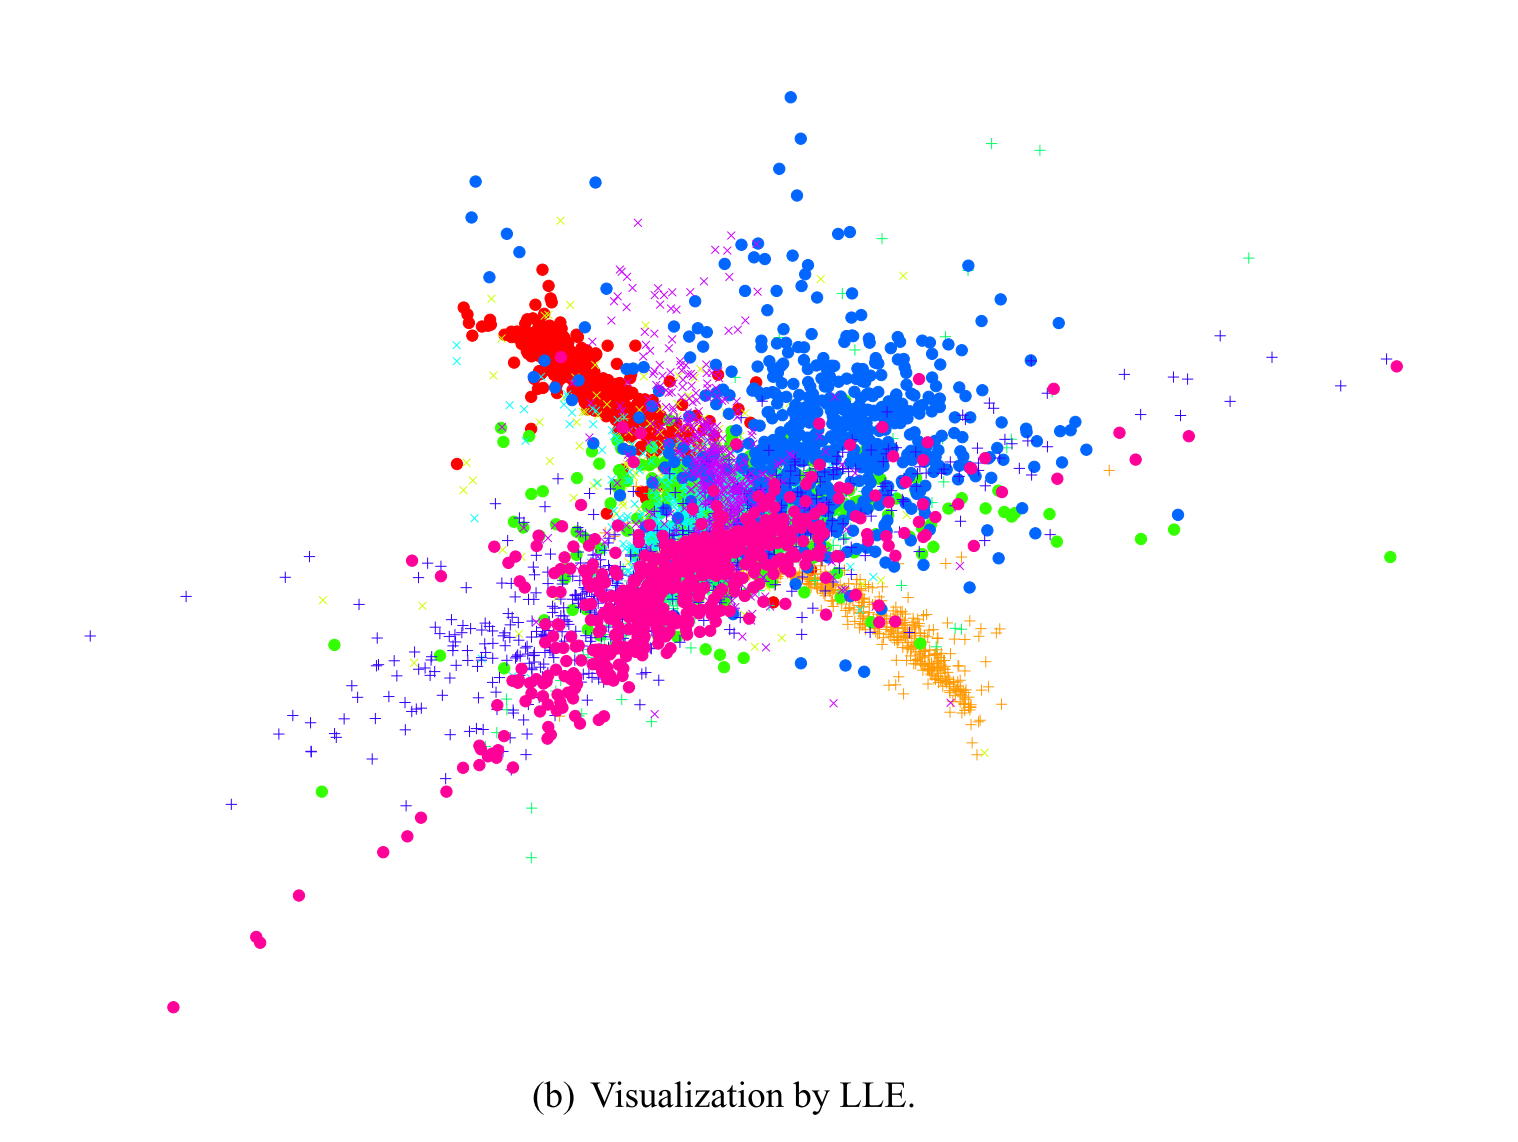
\includegraphics[width=0.3\textwidth]
    				{img/hinton_lle.png} 
    			}}%
    			\caption{MNIST - a Locally Linear Embedding}%
    		\label{fig:3nn}
	\end{figure}	 
 		
		\par 
		In addition to Sammons mapping described above, \cite{VanderMaaten2009} also sites a number of other non-linear dimensionality reduction techniques that aim to preserve the local structure of data including; \textit{Curvilinear Component Analysis} \cite{Demartines1995}, \textit{Stochastic Neighbour Embedding} \cite{Hinton2002}, \textit{Isomap} \cite{Tenenbaum2000}, \textit{Maximum Variance Unfolding} \cite{Weinberger2004}, \textit{Locally Linear Embedding} \cite{Roweis2000}, \textit{Laplacian Eigenmaps} \cite{Belkin2002}.

		\par 
		These techniques all perform well with artificial datasets, however are criticised for not being capable of retaining both local and global structure in a single data map. Even semi-supervised variants are not capable of separating simple datasets such as MNIST into it's natural clusters \cite{Song2007}. Neural network data often requires the retention of both of these, and \cite{Maaten2008} descibes a solution to this problem in the form of \textit{t-Distributed Stochastic Neighbour Embedding}.

	 		
 \subsection{t-Distributed Stochastic Neighbour Embedding}
 \textit{t-Distributed Stochastic Neighbour Embedding} \cite{Maaten2008} has provided a successful and widely used alternative to the dimensionality reduction problem. tSNE, as it is abbreviated, captures much of the local structure of high-dimensional data, while also revealing global structure such that the presence of clusters at several different scales can be observed.
		\par 
		
	\begin{figure}[H]
    			\centering	
			{{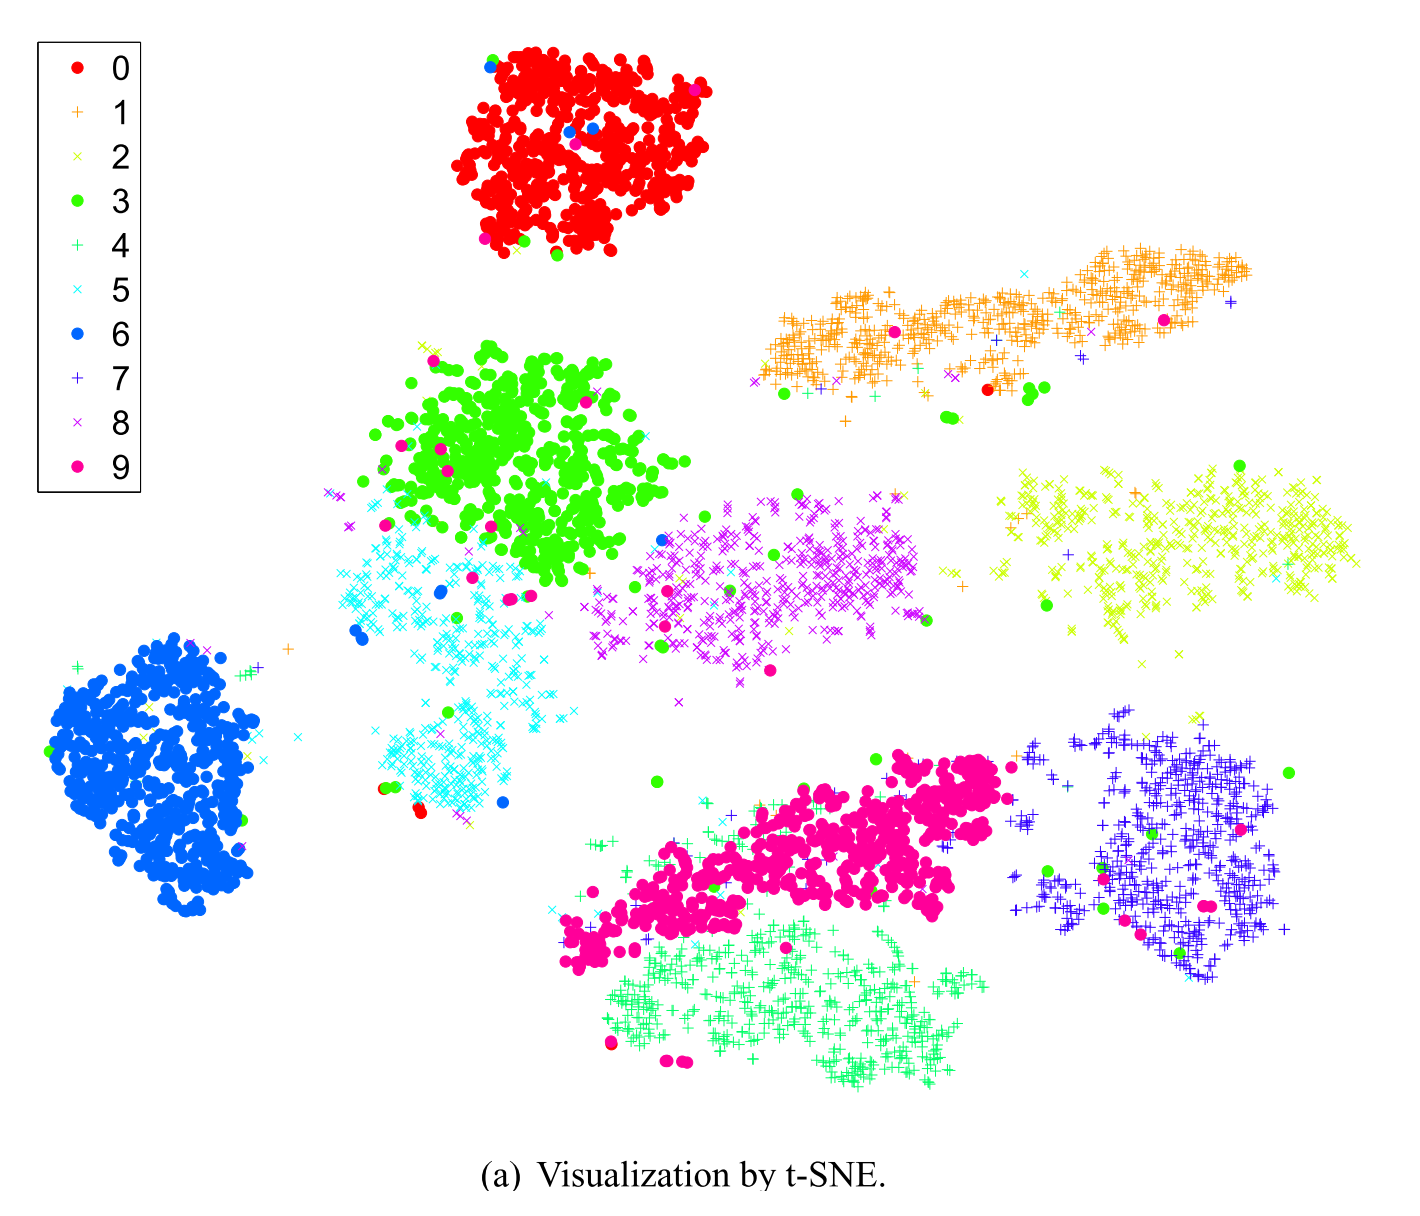
\includegraphics[width=0.3\textwidth]
    				{img/hinton_tsne.png} 
    			}}%
    			\caption{tSNE}%
    		\label{fig:3nn}
	\end{figure}	  
	
		tSNE can therefore be viewed as preserving the `topology' of the data, which as explained previously is incredibly important if the representations formed by these networks are to be successfully captured. tSNE works by constructing for every data point a notion of which other points are it's `neighbours' and tries simultaneously to ensure that all points in the data have the same number of neighbours. In this sense is a lot like a nearest-neighbour graph, however instead having a set number of neighbours connected by edges, and non-neighbours for which there are no connections, data points in the tSNE reduction have a continuous spectrum of neighbours, for which they are neighbours to different, non-binary, extents. This makes tSNE very powerful in revealing global clusters and local sub-clusters within the data - which is ideal for working with complex neural network activations that display both.
		\par
		 The one downside of tSNE is that it's prone to getting stuck at local minima, and due to it's increased complexity is more computationally expensive to run. Changes cannot be made and visualised in real time on standard machines and can take any number of hours, or days even, to produce.  
		 
	\subsection{Evaluation}
	Not one of the dimensionality reduction techniques mentioned appears to be superior. They are largely complimentary, and the choice of which to use intuitively depends on the needs of the data-set and the usage scenario. 
	\par 
	Each has it's own trade off as there can be no exact mapping from high-dimensional space to low dimensional space. 
		\par 
		PCA preserves linear structure, MDS preserves global geometry and tSNE tries to preserve a topological neighbourhood structure.
		\par 
		For the remainder of this project, the data produced by the neural networks will be reduced in dimensions using the tSNE algorithm however, or a faster derivative Barnes-Hut-SNE \cite{VanderMaaten2013}.
		\par 
		Looking into neural networks it is unclear what exactly researchers might be looking for, be it variance, local structure, global structure, or some unknown. tSNE preserves the overall topological structure and thus provides a good solution to this problem. 
\clearpage

\section{Iteration 1 - Animation}
	\subsection{Introduction}
	Reducing the dimensionality of our data enables us to plot the activations in a human comprehensible way, but is in itself not enough. While it is possible to simply plot everything, the sheer number of tSNE plots would quickly put us back in the position of being unable to compare data due to an overloading of information. 
	\par 
	Instead, by looking back to Edward Tufte's principles of visualisation and observing those which have not achieved, the solution becomes immediately obvious: animate the data thus condensing a large number of tSNE plots into short films where patterns can be quickly observed.
	\par 
	
	\begin{figure}[H]
    			\centering												{{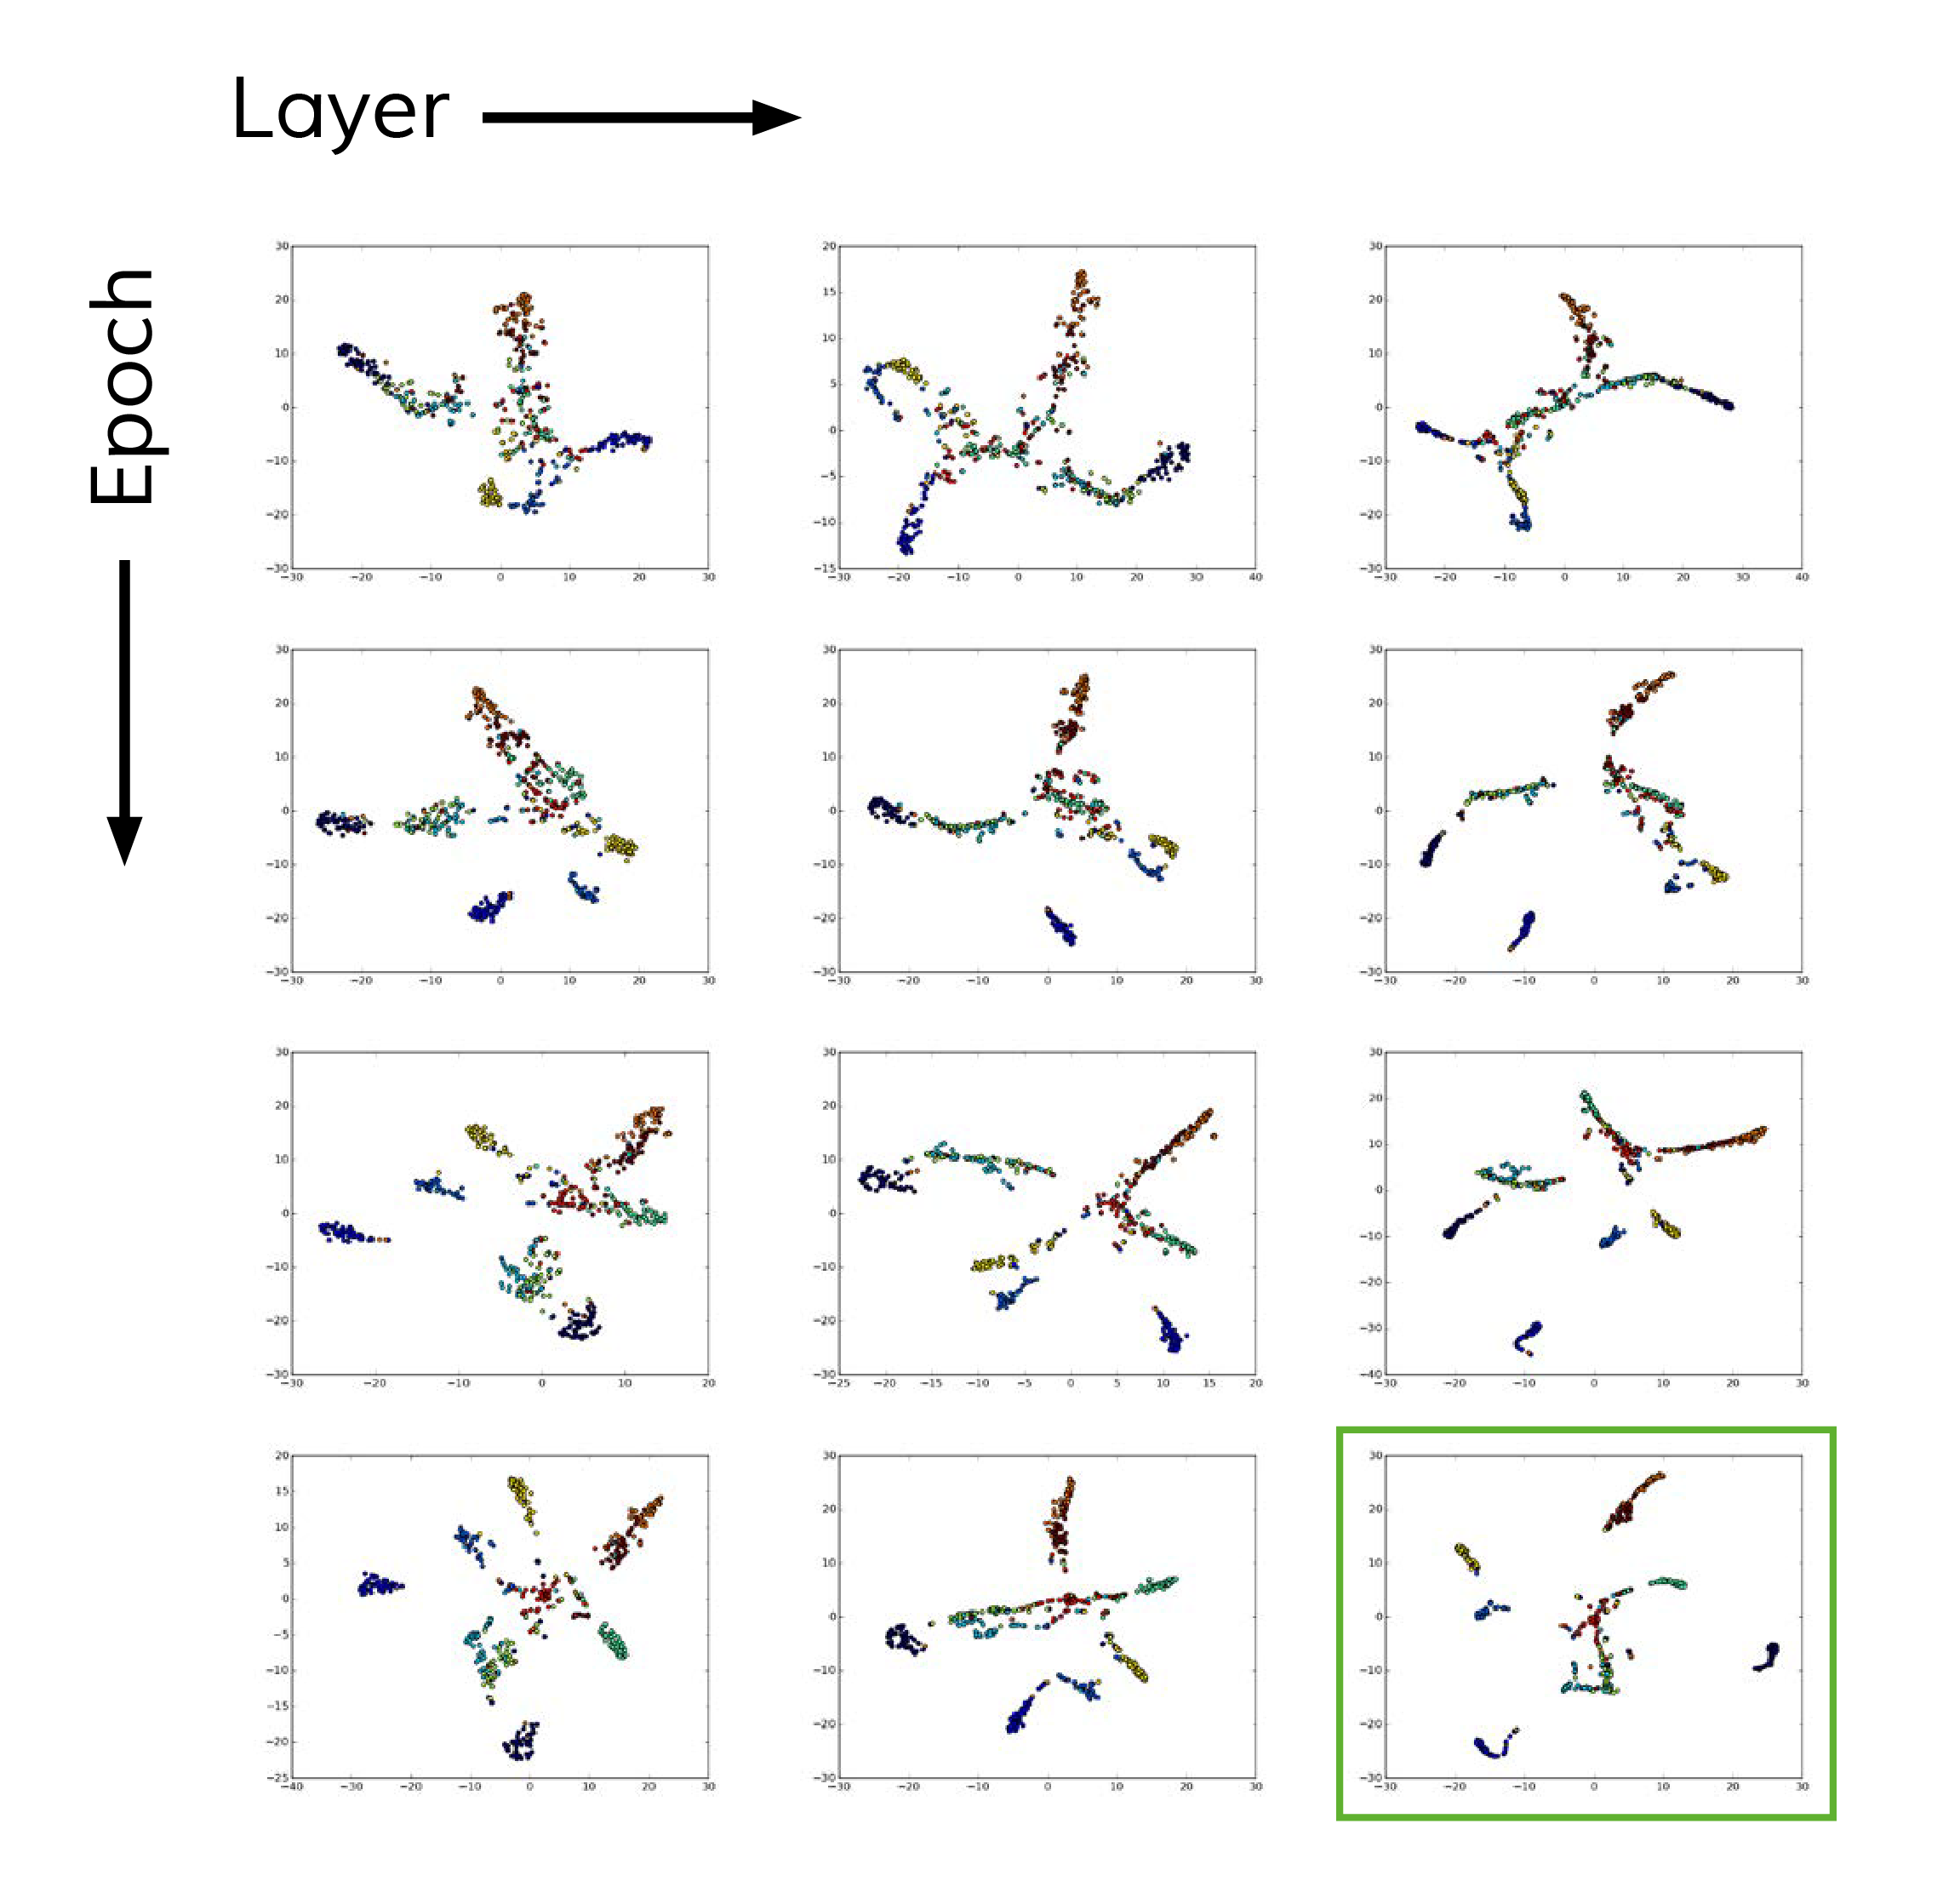
\includegraphics[width=12cm]
    				{img/developing_tsne-01.png} 
    			}}%
    			\caption{Already in the highlighted image it's clear to see the network is learning to distinguish between classes}%
	\end{figure}	

	
	\subsection{Design}
	User interface components for the tool were sketched and evaluated in response to the needs of neural network researchers and in relation to visualisation best practices. 

	\begin{figure}[H]
    			\centering	
    			\subfloat[Initial Sketch]								{{\includegraphics[width=0.4\textwidth]
    				{img/SKE-iter1.png} 
    			}}%
    			\qquad
    			\subfloat[Screenshot]
    			{{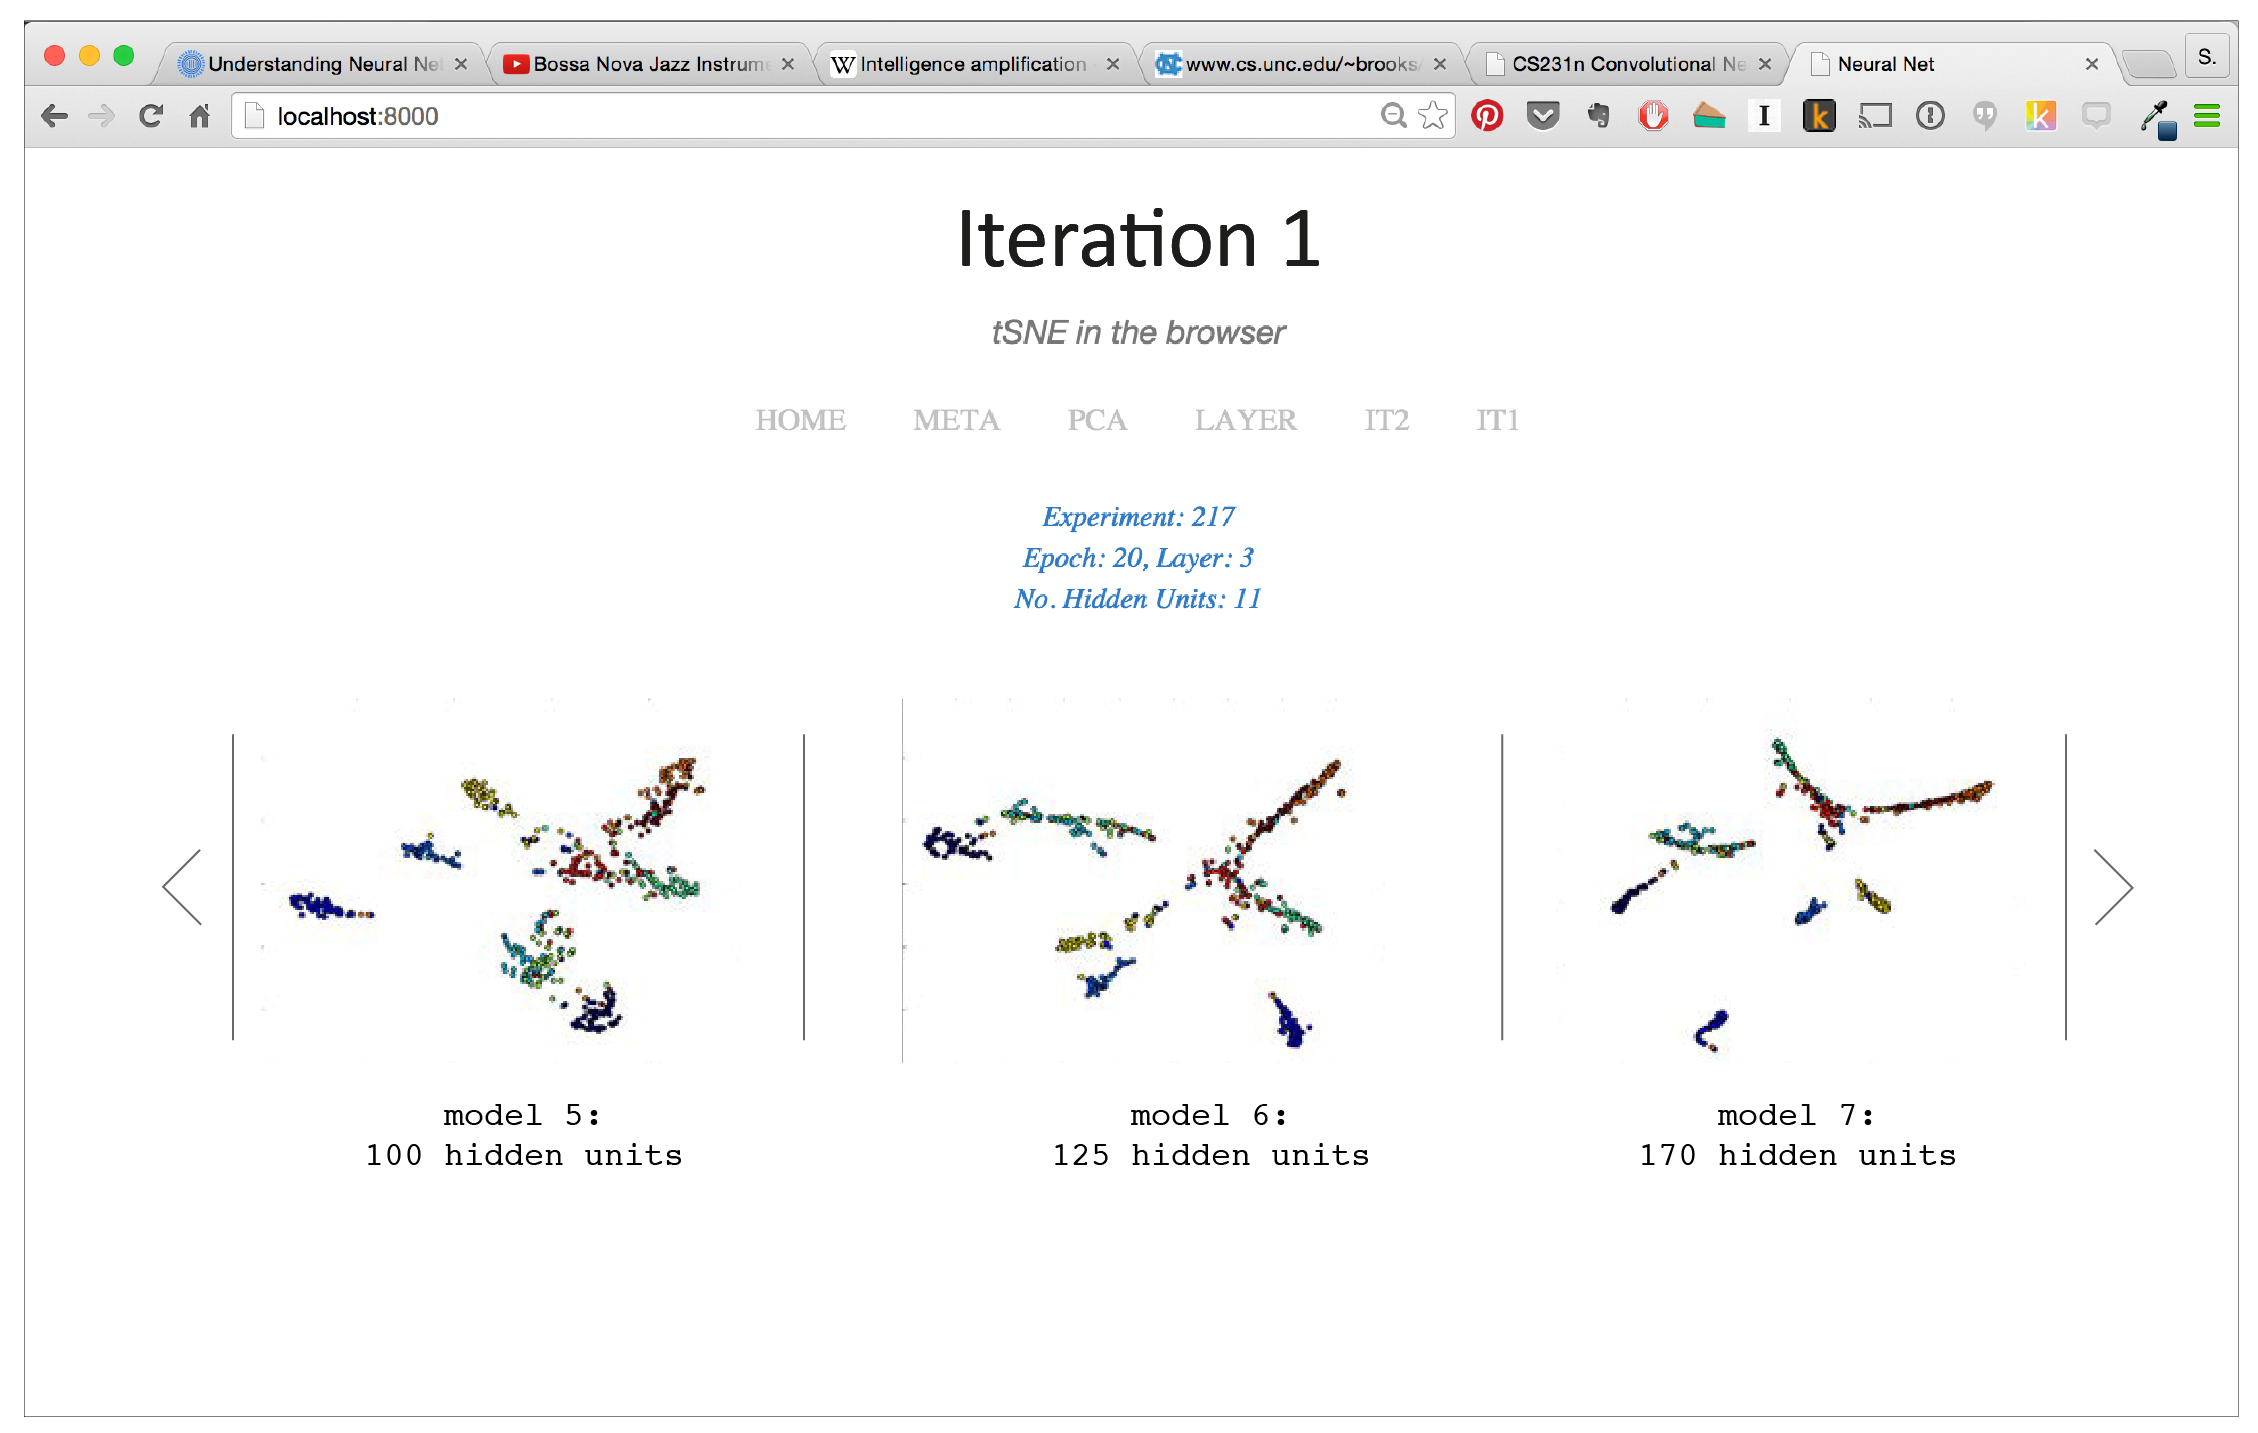
\includegraphics[width=0.4\textwidth]
    				{img/screenshot_it1-01.png} 
    			}}%
    			\caption{ }%
    			\label{fig:design}
		\end{figure}	
	
	This images above show the animations running past the researcher on the screen after they have automated the testing of various models. With a number of animations sitting side-by-side the researcher can observe whether the networks improve across the parameter tuning domain, or not, and can observe emerging patterns within the animations themselves.
	
	\subsection{Architecture}
	This early iteration was developed in a lightweight manor in keeping with the \textit{lean product development} methodology \cite{Blank2013}. This development style states that a \textit{Minimal Viable Product (MVP)} should be built when testing ideas to enable fast testing and learning, which can then be reapplied to the product later without fear of completely rewriting the entire product - something that occurred several times through this project.
	\par 
		
	\begin{figure}[H]
    			\centering												{{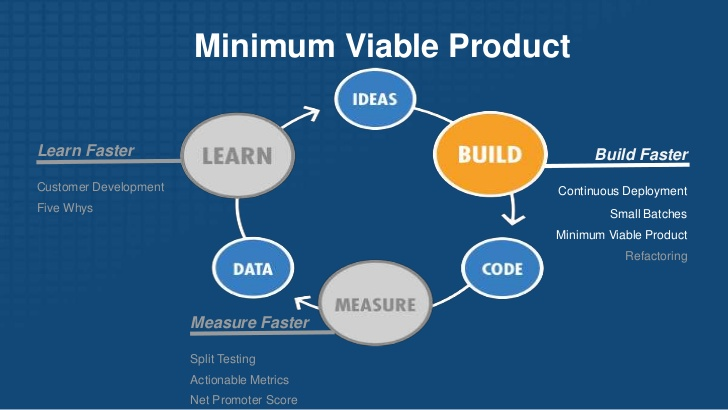
\includegraphics[width=10cm]
    				{img/lean_development.png} 
    			}}%
    			\caption{Lean Development Cycle}%
	\end{figure}	
	
	Here the MVP was a \textit{Python} function that could be copied into the researchers neural network and would automatically run after the network had completed training. The implementation extracted the tSNE plot coordinates from the MongoDB database, processed them using the \textit{numpy} library into a format that could then be processed with another Python library designed for making films, \textit{MoviePy} \cite{?}, which transformed the \texttt{numpy array} of two dimensional tSNE coordinates into a chronologically ordered, by epoch, \texttt{.GIF} animation. These GIF's were stored locally and could be displayed as desired.
	
	\begin{figure}[H]
    			\centering												{{\includegraphics[width=4cm]
    				{img/UML_it1.png} 
    			}}%
    			\caption{UML Snippet: Animation Processing}%
	\end{figure}		

	
	\subsection{Evaluation}
		
	\subsubsection{Neural Network Perspective}
	Unfortunately it was not possible to get a large range of feedback on this iteration due to time constraints, however the little feedback that was attained from fellow students researching with neural networks suggested that this version provided \textit{``pretty"} images to look at, but nothing particularly useful. In particular the following reasons for this were:
		\begin{itemize}
			\item The lack of ability to pause the animations to better understand stand-out abnormal tSNE plots. This was possible by looking back into the file directory of saved backup plots, however provided too much friction for any reasonable use case scenario.
		\item Even with the ability to pause, the animated clips were not of high enough resolution, so where a researcher to stop the animation, not much could be discovered anyway.
		\end{itemize}
		
		\subsubsection{Visualisation Perspective}
		From a visualisation standpoint, as assessed in accordance with Tufte's principles, the animations were far more successful than the previous stand alone images, and allowed the following Tufte principles to be satisfied: 
	\begin{itemize}
		\item Through the animation of tSNE plots across epochs and layers, Edward Tufte's eighth principle to \textit{encourage the eye to compare different pieces of data} is now satisfied. The animation naturally encourages the eye to observe differences in the data as it can be seen to transform from one spatial formation to another. 
		\item Tufte's seventh principle to \textit{augment short term memory through visual patterns} is also satisfied. While it was possible previously to compare tSNE plots by flicking through several images, this process is automated in a  continuous fashion which, as is often referenced in visualisation theory, leaves an imprint on the retina of the previous image thus augmenting short term  memory with the visualisation. 
	\end{itemize}
		\par 
		In response for the call to interrogate the data more closely, it was decided that a key improvement would be the ability to zoom in and out of the data without loss of image quality.
		
		\subsubsection{Implementation Perspective}	
		As mentioned previously this implementation was an \textit{MVP} solution that could enable a successful iterative process. This gave enough insight to indicate that everything should become easily accessible under one package, rather than requiring the researcher to grapple with many implementation details.

\clearpage 

\section{Iteration 2 - Online \& interactive}
	\subsection{Introduction}
	The second iteration focussed on placing the previous processes online and enable the interactive plots needed for a closer inspection of data.
	\par 
	Iteration two used an all JavaScript development stack to collect the activation data, pass it to the client side, and then use a JavaScript implementation of the tSNE algorithm to plot each of the interactive graphics. Each plot would grow as the tSNE cost function was fitted, and researchers could then zoom in or out at any given point to analyse the local or global structure of the emerging tSNE plot.
	
		\begin{figure}[H]
    			\centering	
    			\subfloat[]								{{\includegraphics[width=0.2\textwidth]
    				{img/Iter2_30_53.png} 
    			}}%
    			\qquad
    			\subfloat[]									{{\includegraphics[width=0.2\textwidth]
    				{img/Iter2_30_59.png}
    			}}%
    			 \qquad
    			\subfloat[]									{{\includegraphics[width=0.2\textwidth]
    				{img/Iter2_31_12.png} 
    			}}%
    			\caption{Screenshots of growth from iteration two}%
    			\label{fig:iter2}
	\end{figure}	
	
	\subsection{Design}
	Where the previous iteration focused on inter-model differences, this iteration was influenced by Andrej Karparthy's tSNE visualisations where the model is visualised over the short duration of fitting. As the tSNE cost function is optimised, the visualisation changes - appearing as a series of animated steps. As shown in the initial sketch designs below the aim was to show how tSNE representations were gradually formed.
	\par 
	The two early sketches below demonstrate how the iteration would look if developed beyond the testing point reached. Here the researcher would be able to select the model, epoch and layer corresponding to the tSNE plot they wanted to interrogate, and the interactive functionality would allow them to do so far more effectively than before.

	\begin{figure}[H]
    			\centering	
    			\subfloat[Using Angular.js Repeat with Dropdowns]								{{\includegraphics[width=0.4\textwidth]
    				{img/SKE-iter2-A.png} 
    			}}%
    			\qquad
    			\subfloat[Using Angular.js Sliders]									{{\includegraphics[width=0.4\textwidth]
    				{img/SKE-iter2.png}
    			}}%
    			\caption{ }%
    			\label{fig:iter2}
	\end{figure}		
		
	\subsection{Architecture}
	In order to bring the content online the \textit{MEAN} development stack: Mongo (for the database), Express (for the routing), Angular (for the front-end interaction) and Node (the server), was used. In addition, in order to produce the much called for SVG plots the \textit{D3.js}, or \textit{Data Driven Documents} library was used. 
	\par 
	With the rest of the project written in JavaScript, it became clumsy to interact with the Python tSNE algorithm. For this reason \textit{tSNE.js}, a JavaScript implementation of the tSNE algorithm produced by Andrej Karpathy, a Stanford PhD student, was used. This second implementation followed the example provided by Karpathy online in order to produce the tSNE plot that grows over time \cite{karpathy}. Below is his example used with word-embeddings, where words from a vocabulary are mapped to vectors of real numbers in a low dimensional space.
		
	\begin{figure}[H]
    			\centering												{{\includegraphics[width=7cm]
    				{img/karpahy_tsne.png} 
    			}}%
    			\caption{Andrej Karpathy Implementation}%
	\end{figure}		

	Below is the D3.js, tSNE.js class that implemented this transformation of data. 
	
	\begin{figure}[H]
    			\centering												{{\includegraphics[width=4cm]
    				{img/UML_it2.png} 
    			}}%
    			\caption{UML Snippet: Visualisation}%
	\end{figure}
			
	\subsubsection{Node Server}
	\textit{Node.js} was used in this iteration of the product as the backend server. It is a platform built on Chrome's JavaScript runtime for easily building fast, scalable network applications. Node.js uses an event-driven, non-blocking I/O model that makes it lightweight and efficient, perfect for data-intensive real-time applications such as neural network visualisations.
		\par 
		In 2011, a package manager was introduced for Node.js library, called \textit{npm}. The package manager allows publishing and sharing of open-source Node.js libraries by the community, and simplifies installation, updating and un-installation of libraries \cite{Dahl2009}.
		\par 
		The purpose for using Node was to ensure if the project were to be developed further the useful \textit{node package manager}, npm, could be used to easily distribute the tool amongst the community. Indeed, npm is already a common method of sharing proprietary neural network software within the deep learning community.
		 
		\subsubsection{D3 Visualisation Library}
		D3.js, or Data Driven Documents, is a JavaScript library for producing dynamic, interactive data visualizations in web browsers.
		\par 
		D3 allows the binding of arbitrary data to a Document Object Model (DOM), and then apply data-driven transformations to the document. For example, you can use D3 to generate a HTML table from an array of numbers, or use the same data to create an interactive SVG bar chart with smooth transitions and interaction\cite{Bostock2011a}.
		\par
		D3 is extremely fast, even when using large datasets, making it ideal for working with the large output of the neural networks. The dynamic behaviours enabled for interaction and animation make it highly suited to the tasks in this project.
		\par 
	D3 uses a sophisticated method of joining data with the DOM. With three simple commands (Enter, Update, Exit) D3 enables the programmer to explain a relationship between the data and the scalable vector graphic. For example, a programmer might declare that circle elements should correspond to data, such as in a scatter plot. This contrasts with the more sequential process commonly used where a program may be written to create circles, collect all the circles and then finally assign each data point to a circle.
	
	\begin{figure}[H]
    			\centering												{{\includegraphics[width=7cm]
    				{img/d3enterupdateexit.png} 
    			}}%
    			\caption{D3 Data Binding}%
	\end{figure}	
	
	Data points, such as the coordinates in a tSNE plot, that are joined to existing circles produce the update selection. While unbound data (data for which there are no circles) produce the enter selection. Then, any remaining unbound circles produce the exit selection, where they are often removed. The significance of this is that a scatter plot such as those used in this project can be created with not much more code that the following:
	
	\begin{figure}[H]
    			\centering												{{\includegraphics[width=7cm]
    				{img/d3codeenterupdateexit.png} 
    			}}%
    			\caption{D3 managing data responsively with ease}%
	\end{figure}	
	
	The simplicity of the D3 library is what makes it so powerful, and it was chosen in this project for that reason. Ideally with an implementation started in d3.js, other researchers can build upon the software with relative ease to continue to create extensions to this tool. 
	\par 
	The following images show the tooltips used in the second iteration of the project and the relative ease at which they can be encoded.
	
	\begin{figure}[H]
    			\centering	
    			\subfloat[Text-tooltips]								{{\includegraphics[width=0.35\textwidth]
    				{img/tooltip-text-iter2.png} 
    			}}%
    			\qquad
    			\subfloat[Easily adaptable Tooltip d3.js Code]									{{\includegraphics[width=0.4\textwidth]
    				{img/tooltip_code.png}
    			}}%
    			\caption{ }%
    			\label{fig:iter2}
	\end{figure}	


	\subsection{Evaluation}
		
	\subsubsection{Neural Network Perspective}
		It was agreed that this implementation was far superior to the GIF animations. The ability to zoom and interrogate data at different scales was welcomed, and the retention of quality in doing so was also a marked improvement.
		\par 
		The simple use of tooltips to display the actual value of the data, rather than just using colour, was a great addition as it allowed a researcher to first zoom in on some unlikely data samples and then see which exact data samples were causing the problem.
		\par 
		While the product was deemed to be a marked improvement on the previous iteration, there were still an number of suggested improvements.
		\par 
		The version was criticised for taking too long to process each tSNE plot. This made it hard for researchers to flick between layers or epochs in order to start identifying patterns - and violates Edwards Tufte's seventh principle that visualisation should augment short term memory through visual patterns. Here, the patterns emerged too slowly thus providing an ineffective means of comparison. The slow result is likely due to the slow performance of the client side implementation of the tSNE.js algorithm which wasn't designed for JavaScript.
		\par 
		While the tooltips provided a useful way of understanding which output classification in the range of one to nine was being represented, they were ineffective in demonstrating exactly which input values were causing this classification decision. 

		\subsubsection{Visualisation Perspective}
		Significant visualisation improvements were made through the use of \textit{D3.js} transitions to smooth over the difference between each step in the iterative refinement of the tSNE plot. These transitions are typically used for added effect or embellishment, however in this instance they provide an important functional use - allowing the eye to easily follow specific points trajectories in space. This is useful in allowing the researcher to observe anomalies or peculiar changes in the data over time.	
	\par
	 Also, in addition to the principles held in iteration one, two more Tufte principles were achieved. 
	\begin{itemize}
		\item Through the use of \textit{tooltips}, an often used user interface element that provides more information about a topic upon hovering a computer mouse over the item of interest, satisfying Tufte's sixth principle to \textit{visually highlight your message}. 
		\item In addition, where previously with the animations there was no way to dig into the data without decreasing quality cause by low resolution videos - the capability of the browser to handle \textit{Scalable Vector Graphics, SVGs} enables the researcher to zoom in on the large data sets to observe the local structure captured by tSNE, and to zoom out observing global structure. This allows us to achieve another one of Tufte's principles of quality visualisation  \textit{``Reveal the data at several levels of detail"}. 
	\end{itemize}
	
\subsubsection{Implementation}
The use of the MEAN stack and D3.js were important additions to the development stack and enable the tool to be more effective through lossless rendering and interactivity.
\clearpage 
				
\section{Iteration 3 - Epochs \& Layers}
	\subsection{Introduction}
	Where the previous iteration focussed on the tSNE optimisation of a single layer of activations output from a specific model, epoch and layer, the new version gives control from a model-level, enabling quick switching between epoch and layer. First the researcher selects a model, then on the visualisation page uses a control-box with layer along the x-axis, and epoch across the y-axis to preview the tSNE plot corresponding to the layer-epoch selected.
	\par 
		
	\begin{figure}[H]
    			\centering	
    			\subfloat[]								{{\includegraphics[width=0.45\textwidth]
    				{img/layer_epoch.png} 
    			}}%
    			\qquad
    			\subfloat[]									{{\includegraphics[width=0.45\textwidth]
    				{img/layer_epoch2.png} 
    			}}%

    			\caption{Screenshots of the final product with the control plot on the left, and display plot on the right}%
    			\label{fig:pca_varimax}
	\end{figure}
	
	Within the display box, the new tSNE plots are rendered using d3.js, retaining the ability to zoom in and out upon the data and interrogate individual points. In addition, the d3 transitions are now being used to show how individual data-points are moving between layers and epochs rather than simply across the tSNE optimisation process.
	\par 
	This allows researchers to answer a number of questions very rapidly. For example, observing changes across layers may demonstrate if the back-propagation algorithm is successfully penetrating all layers and producing different representations. Observing changes across epochs demonstrates whether these layers are learning over time, or if they are simply arbitrarily translating the data in space in ways that doesn't amount to learning anything new.
	\par 
	Another change is the addition of image tooltips to map the data points exactly to the input data by showing the input image that each data point represented as a HTML5 canvas rendering. This is particularly useful in allowing researchers to make sense of commonly misclassified data points, such as sevens with ones, or eights with threes.
	
	\subsection{Design}	
	There are two important design elements within this iteration: the control scatter plot that the researcher uses to select the corresponding tSNE plot, and the display scatter plot, tSNE plot, that the researcher can interrogate by zooming in to observe local patterns, zooming out to observe global patterns, hovering over points to see which input they correspond to and as the control plot is panned over also observe as the individual points get reorganised into different structures.
	\par 
	A number of different methods were tried for the control unit, including using Angular.js sliders, check-boxes and drop down menus. However these all failed to unify the transition that was occurring; they failed to highlight where exactly a layer-epoch combination sits with respect to any other layer-epoch combination - something that the user interface element decided upon did well, a simple scatter plot. In addition the scatter plot enabled the product to have consistency in its visual form.

	\begin{figure}[H]
    			\centering												{{\includegraphics[width=7cm]
    				{img/SKE-iter3-C.png} 
    			}}%
    			\caption{Wireframe Design}%
	\end{figure}	
	 
	The new use of D3.js transitions was to animate the change from one representation of a data point (or datum) to another via a number of rendered transition states. This allows the human eye to follow how specific points move with ease, and enables us to fulfil more of Tufte's guiding visualisation principles to \textit{augment short-term memory loss with visual patterns} - here the transitions literally allow us to follow specific data points as they move across the screen.
	\par 
	
		\begin{figure}[H]
    			\centering	
    			\subfloat[Barnes Hut SNE after applying to the imagified scatterplots]								{{\includegraphics[width=0.3\textwidth]
    				{img/d3Transitions.png} 
    			}}%
    			\qquad
    			\subfloat[Barnes Hut SNE after applying Principle Components Analysis]									{{\includegraphics[width=0.4\textwidth]
    				{img/SKE-iter3-D.png} 
    			}}%
    			\caption{}%
    			\label{fig:epoch_layer}
	\end{figure}

	D3.js has yet another very useful tool \texttt{d3.scale.linear} which essentially normalises the data within the visual range on the screen. Mapping the input domain to the output range, and thus fitting the data so the user doesn't have to worry about data distortion. 
	
	\begin{figure}[H]
    			\centering												{{\includegraphics[width=7cm]
    				{img/d3scales.png} 
    			}}%
    			\caption{d3 scaling elements}%
	\end{figure}	
		
	\subsection{Architecture}
	
		\subsubsection{Entirely Python} 
	In iteration three, the node.js and express.js back-end components used previously were replaced with Python's \textit{Flask}, a \textit{Sinatra}-like micro web application framework written for Python.  The framework is used by companies such as Pinterest and LinkedIn and serves as a far more appropriate product for the back-end.
	\par 
	The entire architecture has now been streamlined with a Python only back end; from the neural network, to the database, to the RESTful server and post-processing functionality. The entire front end is JavaScript using Angular.js for basic manipulation of the DOM and d3.js for the interactive visualisations. They speak to each other through a very basic RESTful API.
	\begin{figure}[H]
    			\centering												{{\includegraphics[width=7cm]
    				{img/Flow_diagram-01.png} 
    			}}%
    			\caption{The architecture behind the whole system}%
	\end{figure}	
	
	\subsubsection{Streamlined Database}
	In addition to the restructuring of the architecture to have a clearer divide between back-end Python and front-end JavaScript - the MongoDB database is now manipulated using a python toolkit \texttt{PyMongo}. 
	\par 
	This opportunity allowed a streamlining of the database structure as well, from the model represented in the ER schema at the beginning of the report to the following, perhaps slightly clumsier, however far easier to interact with JSON storage format - stored in Mongo's \textit{BSON} format.
	\par 
	This new database schema stores important parameters for understanding the neural network, as well as the key data required for the visualisations.
	
	\begin{figure}[H]
    			\centering												{{\includegraphics[width=4cm]
    				{img/UML_data.png} 
    			}}%
    			\caption{UML Snippet: PyMongo Interaction}%
	\end{figure}		
	
	\begin{figure}[H]
    			\centering												{{\includegraphics[width=9cm]
    				{img/actual_json.png} 
    			}}%
    			\caption{Simplified JSON scheme for PyMongo}%
	\end{figure}
	
	\subsubsection{Tooltip Adaptation}
A small change made to the text tooltips was the addition of a fill to the background - enabling the text to pop out.
	\par 
	
	\begin{figure}[H]
    			\centering												{{\includegraphics[width=5cm]
    				{img/tooltip-text-iter3.png} 
    			}}%
    			\caption{Tooltips}%
	\end{figure}	
	
	However a more major change was the addition of image-tooltips. Initially this involved trying a number of options that involved the uploading of \texttt{.png} images rendered each time the researcher hovered over a point. This was slow and damaged the rapid interaction afforded through the use of d3.js. 
	
	\begin{figure}[H]
    			\centering												{{\includegraphics[width=5cm]
    				{img/tooltip-image-iter3.png} 
    			}}%
    			\caption{Chris Olah adopted image tooltips}%
	\end{figure}	
	
	\par 
	After some unsatisfactory attempts and exploration of other methods, the method used in Chris Olah's blog post \cite{Olah2014c} was discovered. It took a substantial amount of time to decipher how the implementation worked, however it used the same \texttt{base64} arrays that had been used previously to store the MNIST dataset in the Mongo database, and used \textit{HTML5 Canvas} to render the points in the browser. The length of the input (784 pixels) was used to index the array and render it live.
	\par 
	Initially Olahs code was hacked onto the visualisation code from the previous iteration, however this was unsatisfactory and bug-prone. Fortunately Olah had also implemented a version of the scatter plot for another post, all be it in a rather complex way, so it was decided to use the majority of his code governing the scatter plot and the tooltips, and build upon that to create the interactive.	

	\subsection{Evaluation}
		\subsubsection{Neural Network Response}
		This new product is a vast improvement towards achieving the goals set out. Enabling researchers to process information by epoch and layer has clear advantages:
		\par 
		A researcher may compare an earlier epoch with a later one. If the externally measured loss values had started to plateau, the researcher would expect that the network wasn't learning much. However with the ability to look into the data, the researcher might observe that the network is actually trying to classify one hard example continually reshaping the space around it, and in a few more hundred epochs could learn to classify this example that doesn't contribute much to the error but which is actually a very important example to classify. Consider Google's own algorithms that left them classifying people with black skin as monkeys - a severe mistake that could potentially be identified with this tool.
		\par 
						
	\begin{figure}[H]
    			\centering												{{\includegraphics[width=13cm]
    				{img/sne_plot_E2_l1.png} 
    			}}%
    			\caption{Epoch 2, Layer 1 from different models: demonstrating how vastly different models representations of the data can be}%
	\end{figure}	
	
		A researcher may also look by layer to check that activations are indeed propagating from one layer to the next; serving as a proxy to see that the network is actually adjusting the weights later in the network. It's a common, and sometimes hard to diagnose problem, if weights are not changing sufficiently due to poor network initialisation or some other complication. Again, the tool performs excellently for such a task.
		\par 
		However, after observing that several of the tSNE plots appeared to simply be rotations of one another it was questioned whether researchers would accurately be able to diagnose which changes were the neural network actually learning, and which were simply transformations in space. For example, a network in epoch four could have a plot that appears to face north, then at epoch eight, south, and again at epoch twenty four, north. Here there is a full rotation of the data where nothing new is being learnt, however due to the control implementation of panning across epochs and layers it's unlikely that the researcher would be able to pick this up any ease. 	
		
		\subsubsection{Visualisation Response}
		The key visual changes here were the re-implementation of transitions between layers and epochs enabling the researcher to observe patterns more accurately, and in addition ensuring that Edward Tufte's guide was still being followed.
		\par 
		The other major change was the introduction of the image tooltip. Previously the text-tooltip enabled the researcher to view the classification result however here each data point directly corresponds to one of the input values, each of which is individually rendered in the browser. This adaptation of Chris Olahs blog post provides a much needed extra dimension of exploration within the project.
	\subsubsection{Implementation Response}
	There were a number of significant implementation changes in iteration three; a more streamlined database and a properly separated Python back-end and JavaScript front-end. This makes for cleaner interaction within the backend and between the backend and frontend through the RESTful API. In addition the adapted visualisation infrastructure makes it easier for researchers to interact with in the future.
	
	\begin{figure}[H]
    			\centering												{{\includegraphics[width=14cm]
    				{img/UML_d3.png} 
    			}}%
    			\caption{Adapted \& Extended Olah D3.js visualisation implementation}%
	\end{figure}	

	\clearpage 
	
\section{Iteration 4: metaSNE \& Principle Component Analysis}
	
	\subsection{Introduction}
	Iteration four addresses the problem discovered through iteration three of rotational data. The main focus therefore of this section is an exploration into methods for mapping that rotational data to a space that enables researchers to better decipher it. In particular this section looks at principle component analysis, PCA, and Varimax rotation. 

	\subsubsection{Isometries in Representations}
	In the tSNE plots that visualise the representations being formed by the neural networks it's important to distinguish which plots demonstrate new pieces of information being learnt, and which simply appear to be learning however are just translations in space, or are simply \textit{isometries} of one another; rotations or reflections.
	\par 
	In his blog post on \textit{Representations} \cite{Olah2014} explores this notion of isometries stating that for any representation $ X $ there is an associated metric function, $ d_{x} $, which gives us the distance between pairs of points within that representation. For another representation $ Y $, $ d_{x} = d_{y} $ if and only if $ X $ is isometric to $ Y $. This is exactly the form required that can remove isometric data.
		\par 
		This transformation into metric space can be incredibly complex, so the approach taken instead approximates this by using \textit{Principle Component Analysis} to mean centre and find the maximal variance in the data, and \textit{Varimax Rotation} to subsequently orthogonalise the mappings to create a dataset that has isometries which can be easily classified.
		
		\begin{figure}[H]
    			\centering												{{\includegraphics[width=0.4\textwidth]
    				{img/sne_plot_E2_L1_rotation.png} 
    			}}%
    			\qquad
    			{{\includegraphics[width=0.4\textwidth]
    				{img/sne_plot_E2_L3_rotation.png} 
    			}}%
    			\caption{This experiment demonstrates two layers where the data has essentially effectively just been rotated - demonstrating nothing particularly new has been learnt}%
		\end{figure}

	\subsection{Design}
	The fourth iteration of this project is where the development ends. There are still improvements that can be made, and these will be discussed in the concluding section, however by this point there is certainly a tool that can be utilised to make important decisions when training neural networks. 
	\par 
	There are five key components to this final tool:
	\begin{itemize}
		\item First, the neural networks themselves: two neural networks are provided with the tool, a convolutional network and a feed forward network as described in the chapter on data collection. These two classes are easily adaptable under the \textit{Lasagne} guidelines.
		\item Second, the saving functionality afforded by \textit{PyMongo} and the \textit{MongoDB} database that saves key data in an easily accessible format to a local datastore, and all processing functions that allow this to integrate seamlessly with the \textit{Lasagne} neural networks.
		\item Third, the post-processing functionality that provides the PCA-Varimax / meta-SNE plotting explained later in this chapter. 
		\item Fourth, the RESTful API providing data to the client.
		\item Fifth, the front end \textit{Angular.js} and \textit{D3.js} application consisting of an easy to use homepage where the researcher can select the model they want to explore, and the visualisation pages where the researcher can interrogate their data.
	\end{itemize}
	
	Below are two sketch diagrams that demonstrate the simplicity of the front end.
	
		\begin{figure}[H]
    			\centering	
    			\subfloat[Homepage]								{{\includegraphics[width=0.4\textwidth]
    				{img/SKE-iter3-E.png} 
    			}}%
    			\qquad
    			\subfloat[PCA interaction]									{{\includegraphics[width=0.4\textwidth]
    				{img/SKE-iter3-B.png} 
    			}}%
    			\caption{}%
    			\label{fig:pca_varimax}
	\end{figure}
	
	\subsection{Architecture}
	The final architecture retains a number of components that were described in the previous section; however the addition of the Principle Component Analysis and Varimax Rotation post-processing is explored below. 
	\par 
	
	\subsubsection{PCA-Varimax Post-Processing}
	In order to determine the success of the removal of isometric data by the post-processing function, a simplified dataset was created.
	\par 
		
	\begin{figure}[H]
    			\centering												{{\includegraphics[width=7cm]
    				{img/rotatedDataOriginal.png} 
    			}}%
    			\caption{The test dataset}%
	\end{figure}	
	
	The test set, above, was a number of uniformly generated $x$ and $y$ points that when plotted produced a dataset that consists of two identical triangles that had been rotated by differing amounts, and three identical squares that had likewise been rotated by differing degrees with differing offsets. This creates an artificial dataset that makes it easy to determine the success of the post-processing functions, due to our intuitive understanding of triangles and squares.
	\par 
	Three different approaches were used in an attempt to generate an effective \textit{metaSNE} plot:
	\\\
	\textbf{Image Compression \& metaSNE}
	\par
	The first method took influence from the tSNE plots created of the MNIST dataset where each of the 28 pixel by 28 pixel images had their dimensions collapsed into a single 784 pixel array before the tSNE algorithm was applied to the several thousand in the validation dataset.
	\par 
	With the scatter plots, in order to do this, the (x, y) coordinates needed to first be transformed into an image with discrete dimensions. For example, a 500 pixel by 500 pixel image. 
	\par 
	There were a number of different methods that could have been employed here, however the method adopted was the creation of a two dimensional histogram where should a point to appear within a given coordinate bin, then that bin would be assigned the average of all points situated within it.
	\par 
	Once the images were generated, tSNE was reapplied and thereby creating a metaSNE plot.	As can be seen from the figure below this works for the most part due to the relatively high-fidelity of the selected dimensions. However, where two or three points are situated very close together such that they enter the same bin, the transformation taking an average distorts the dataset somewhat representatively. This method proved to be relatively unsuccessful at creating the desired outcome, or metaSNE plots, once tSNE was reapplied.
	
	\par 
	\begin{figure}[H]
    			\centering												{{\includegraphics[width=12cm]
    				{img/2d_historgram_tsne.png} 
    			}}%
    			\caption{Imagifying Scatterplots}%
	\end{figure}	
	
 	\textbf{Principle Component Analysis}
	\par
	The second method attempted was to first apply Principle Component Analysis, PCA, to the scatter plot in an attempt to remove the majority of the rotational differences, and mean-centre the data before the reapplication of the tSNE algorithm upon these plots.
	\par 
	PCA is a statistical procedure that converts the set of points along a number of principle components. The largest principle component has the largest possible variability in the data, and each succeeding component has the highest variance possible under the constraint of those preceding it.
	\par 
	This mapping of plots along principle components should remove the majority of rotational data held within the plots, and worked well as is demonstrated in the plot below on the left.
	\par 
	This second method was far more successful than the first in removing isolemtric data, however upon application of tSNE the points were disappointingly classified.
	\\\
		\begin{figure}[H]
    			\centering	
    			\subfloat[Application of Principle Component Analysis]							{{\includegraphics[width=0.3\textwidth]
    				{img/PCArotations.png} 
    			}}%
    			\qquad
    			\subfloat[Application of Varimax Orthogonalisation]									{{\includegraphics[width=0.3\textwidth]
    				{img/VarimaxRotations.png} 
    			}}%
    			\caption{}%
    			\label{fig:varimax}
	\end{figure}

	\textbf{PCA \& Varimax Rotation}
	\par
	After the unsatisfactory results produced by the PCA process, it was decided that the isometry free datasets needed to be simpler for the tSNE algorithm to map them effectively. 
	\par 
	After much searching, a solution presented itself in the form of \textit{Varimax Rotation} \cite{Lin2010} which orthogonalises the data such that the actual coordinate system is unchanged, but the orthogonal basis that is being rotated is aligned to those coordinates. This produced the plot on the right which aligned the test set perfectly into its original triangles and squares, they were centred directly on top of one another - thus removing the isometric data as desired.
	\par 
	The plot below demonstrates on the left the Barnes Hut SNE output when reapplied simply to the PCA rotated data, and the plot on the right after the data has occurred the Varimax Rotation - the former fails to accurately represent any of the data as similar, while the latter does exactly as desired - separating the squares from the triangles, and demonstrating that they are simply slight variations of one another.

	\begin{figure}[H]
    			\centering	
    			\subfloat[Barnes Hut SNE after applying Principle Components Analysis]									{{\includegraphics[width=0.23\textwidth]
    				{img/BHafterPCAOnly.png} 
    			}}%
    			 \qquad
    			\subfloat[Barnes Hut SNE after applying Principle Components Analysis, and Varimax Orthogonalisation]									{{\includegraphics[width=0.23\textwidth]
    				{img/BHrotations.png} 
    			}}%
    			\caption{}%
    			\label{fig:pca_varimax}
	\end{figure}


	It is this final version: PCA and Varimax Rotation is used in the final tool to enable researchers to get a better grasp upon how similar tSNE scatter plot really are, ensuring for more accurate pattern spotting across a researchers models.
	
	\begin{figure}[H]
    			\centering												{{\includegraphics[width=7cm]
    				{img/UML_plot.png} 
    			}}%
    			\caption{Post-Processing}%
	\end{figure}	
	
	
	\subsubsection{A tool for visualising neural networks}
	The final architecture for the project remains very similar to that of the previous iteration. 
	\par 
	The	hybrid UML, entity relationship, flow diagram below explains the interconnection between the various parts:
	\begin{itemize}
		\item \textbf{Client Side}
			\begin{itemize}
				\item Experiment selection
				\item Visualisation selection
				\item Browse by animation section
				\item Interactive section; where the researcher can explore by Epoch, Layer, PCA/Varimax centred, or pure meta-SNE (tSNE applied directly to tSNE).
			\end{itemize}
		\item \textbf{RESTful API}	
			\par 
			The RESTful API enables the site to load quickly without having to upload vast amounts of neural network data, or heavy image data.  
		\item \textbf{Server Side}
			The server has two primary components: the database and the neural network processing elements. The neural network processing however is split into a further three parts:
			\begin{itemize}
				\item The Neural Networks themselves which can be called from the network automation section.
				\item The helper functions which facilitate the extraction of data from the neural network and store it appropriately
				\item The post-processing unit which extracts from the database all stored tSNE plots, and processes them to produce the data for the meta-SNE plot and PCA/Varimax plots.
			\end{itemize}
	\end{itemize}
	
%	\begin{figure}[H]
%    			\centering								%				{{\includegraphics[width=7cm]
%    				{img/UML_server.png} 
%    			}}%
%    			\caption{Basic RESTful interaction}%
%	\end{figure}	
						
	\begin{figure}[H]
    			\centering												{{\includegraphics[width=14cm]
    				{img/all_combined-01.png} 
    			}}%
    			\caption{UML, ER, Flow diagram hybrid}%
	\end{figure}	

	
\subsection{Evaluation}
These two final screen shots demonstrate the control plot side by side with the display plot. The control has been created using the PCA-Varimax post processing such that points next to one another are similar or may be rotations of one another. The display shows the tSNE data once it has been transformed along the principle components and orthogonalised with Varimax. 
\par 
The homepage is a simple place where the researcher can select a model from the database, which will then be passed up to the client side application and the researcher can browse by either: Epoch \& Layer tSNE, PCA \& Varimax tSNE, or, tSNE tSNE (meta-SNE).

	\begin{figure}[H]
    			\centering	
    			\subfloat[Final PCA exploration]							{{\includegraphics[width=0.45\textwidth]
    				{img/screenshot_home.png} 
    			}}%
    			 \qquad
    			\subfloat[Final Homepage]									{{\includegraphics[width=0.45\textwidth]
    				{img/screenshot_homepage.png} 
    			}}%
    			\caption{}%
    			\label{fig:pca_varimax}
	\end{figure}

	\subsubsection{Neural Network Perspective}
	The response to this final iteration, that effectively ties together the lessons from the previous three, was overwhelmingly positive.
	\par 
	The tool enabled researchers to spot patterns emerging within datasets as networks trained, a sample of which is in the final observations section of this report.
	
	\subsubsection{Visualisation Response}
	From a visualisation perspective this final tool fulfils all of Edward Tufte's visualisation principles to a greater or lesser degree: 
	\begin{itemize}
		\item Principle 1, \textit{show only as much information as required}, is fulfilled comprehensively through the use of the tSNE algorithm which compresses the multi-dimensional data down into the 2D plane.
		\item Principle 2, \textit{include visual difference only when required}, is fulfilled by the PCA-varimax algorithms such that visual differences are not simply `shown when required', but are intelligently organised to enable easier comparison.
		\item Principle 3, \textit{use visual encodings for quantitative values}, in first transforming the multidimensional data down into two dimensions and then using the scatter plot diagram, which even without axis, uses the visual encoding of \textit{spatial separation} to encode the differences in quantitative values.
		\item Principle 4, \textit{differences in visual properties should correspond to actual differences in the data}, is explicitly implemented with the tSNE algorithm which optimises a cost function that aims to preserve the qualities in the data when mapping down to a number of dimensions that can be easily visualised. 
		\item Principle 5, \textit{do not connect values that are discrete}, is realised simply by not making any connections at all, and allowing the researcher to spot these connections of their own accord, helped along by the d3.js transitions and display plots.
		\item Principle 6, \textit{visually highlight the most important part of your message}, occurs at two levels: firstly when the researcher scrolls over a point in the control plot, the display plot changes to the corresponding tSNE plot, and secondly as the researcher scrolls over the points in the display plot, either the categorisation value is displayed as a text string, or the input image is displayed as a HTML5 canvas rendering. 
		\item Principle 7, \textit{augment short term memory through visual patterns}, has been achieved by using transitions from one tSNE plot to another, thus supplementing the researchers short term memory of the previous plot by providing a trajectory for each point which can be followed through the transition.
		\item Principle 8, \textit{Encourage the eye to compare different pieces of data}, is fulfilled by providing the control plot which the researcher can scroll over to rapidly change the tSNE plot on display, thus being able to successfully compare the data, and the PCA-Varimax algorithms which perform complex comparisons of the data creating the PCA plots.
		\item Principle 9, \textit{Reveal the data at several levels of detail}, is enacted by simply enabling the researcher to zoom in and focus on the local structure within the tSNE plot, or to zoom out and focus on the global structure.
		\item Principle 10, \textit{Don't distort the data}, has been fulfilled by using the d3.js linear scaling function that allows us to map data points directly to the visualisation with one constant scale without undergoing distortion. However it is clear that the data has undergone significant distortion by each of the algorithms that enable the visualisation to achieve earlier principles, and so this final principle is fulfilled to a lesser degree.
	\end{itemize}
	
	\subsubsection{Implementation Response}
	The implementation of the final tool clearly separates the concerns of the client side and the server side. It partitions key elements in classes and folders within a clear file-structure, and maintains a clean database structure too. 
	\par 
	This implementation is deceptively simple and should make it easy for researchers to use the tool, or adapt it to their needs.
	
\clearpage 

\section{Conclusions}
	
	\subsection{Final Observations}
	This section explores some of the observations that were made using the tool, exploring the tSNE data across both the epoch-layer control configuration as well as the PCA-varimax control configuration.
	
	\begin{figure}[H]
    			\centering	
			{{\includegraphics[width=0.7\textwidth]
    				{img/conc_X24_H7_L1-3-5_E30.png} 
    			}}%
    			\caption{Exp.24, Hidden Units.7, Layers.1,3,5, Epoch.30}%
    		\label{fig:mnistHinton}
	\end{figure}
	
	\textbf{Layer Change:} \textit{Emphasising Early Error}
	\par
	Above can be seen that as the neural network gets deeper the clusters within the tSNE plots get gradually tighter and more distinct. This indicates a transforming representation that has discovered a space that effectively separates the classes at an early layer, and the subsequent layers appear to be simply emphasising these early lessons.
	\par 
	This observation could lead the researcher to adjusting their model more substantially in the earlier layers - perhaps adding more hidden units, applying more effective drop-out to disassociate the relationships so directly between layers, avoiding what could be an early over fitting of the data.

	\begin{figure}[H]
    			\centering	
			{{\includegraphics[width=0.7\textwidth]
    				{img/conc_X35_H512_L3_E2-40.png} 
    			}}%
    			\caption{Exp.35, Hidden Units.512, Layer.3, Epochs.2-40}%
    		\label{fig:mnistHinton}
	\end{figure}
	
	\textbf{Epoch Change:} \textit{Non-Uniform Distribution}
	\par 
	Above can be seen a successful clustering being developed across the epochs with readings taken across the same layer. The network has performed exactly as desired and separated the digits particularly well into different clusters.
	\par 
	One observation that could enable the researcher to make potential changes to the model are two clusters at the top, and two clusters at the bottom. Here the network is not creating a particularly distinct separation between the digits `7' and `9', and between the digits `3' and `5'. This could lead to the researcher including more examples of these digits in their training-set, or in a convolutional network adjusting the filter and maxpooling parameters, as this could potentially help the network to distinguish between these admittedly similar shapes.

	\begin{figure}[H]
    			\centering	
			{{\includegraphics[width=0.7\textwidth]
    				{img/conc_X35_H512_L5_E2-40.png} 
    			}}%
    			\caption{Exp.35, Hidden Units.512, Layer.5, Epochs.2-40}%
    		\label{fig:mnistHinton}
	\end{figure}
	
	\textbf{Epoch Change:} \textit{Retention of Misclassification}
	\par 
	In this example as the network trains the researcher begins to see a tightening of the clusters in a very distinct manor - forming little c's. The highlighted portion is the retained misclassification of a small number of sevens {\includegraphics[width=0.4cm]{img/seven_one-01.png}}  within a cluster of ones {\includegraphics[width=0.4cm]{img/seven_one-02.png}}.
	\par 
	These classification examples demonstrate why such a network often achieves very good accuracy, however not entire accuracy - the examples are indeed just very similar. In order for the researcher to improve such a network many more training examples such as this would be required - and this tool enables the researcher to discover exactly what these should be.

	\begin{figure}[H]
    			\centering	
			{{\includegraphics[width=0.7\textwidth]
    				{img/conc_X46_H16_L1-3_E6-16.png} 
    			}}%
    			\caption{Exp.46, Hidden Units.16, Layers.1-3, Epochs.6-16}%
    		\label{fig:mnistHinton}
	\end{figure}
	
	\textbf{Layer change \& Epoch change:} \textit{Minimal Learning}
	\par 
	This situation mirrors the above, where sevens are again misclassified as ones - however here the two examples are from different layers as well as distinctly separate epochs. This means that the network is really failing to learn much at all on either account. 
	\par 
	Here the researcher would likely increase the number of hidden units in each layer.


	\begin{figure}[H]
    			\centering	
			{{\includegraphics[width=0.7\textwidth]
    				{img/conc_X49_H64_L1_E14-26.png} 
    			}}%
    			\caption{Exp.49, Hidden Units.64, Layers.1, Epochs.14-26}%
    		\label{fig:mnistHinton}
	\end{figure}
	
	\textbf{Epoch Change:} \textit{Local Reshaping, Global Consistency}
	\par 
	Here are two very similar sets of data looking at the patterns that emerge on the right hand side of each image. However, when observed more closely - and this is far easier to spot using the interactive tool with the transitions - then the reflecting of the section highlighted almost directly along the x-axis can be seen. 
	\par 
	The flipping of this section, and relative retention of the others could suggest that these units are proving a particular problem for the network. It could also prove that the network is happy with the global structure that it has identified - as they are primarily well classified, but not with the local structure, which it is still regularly tweaking.

	\begin{figure}[H]
    			\centering	
			{{\includegraphics[width=0.7\textwidth]
    				{img/conc_X49_H64_L5_E16-28.png} 
    			}}%
    			\caption{Exp.49, Hidden Units.64, Layers.5, Epochs.16-28}%
    		\label{fig:mnistHinton}
	\end{figure}

	\textbf{Epoch Change:} \textit{Lower Half Characterisation}
	\par 
	In this example, the network appears to have learnt to distinctly classify digits 0,1,2,4,7 \& 9 however is having difficulties with 3,5,6 \& 8. Again this would tie into our intuition about these letters that could be described as a whole as \textit{curvy with distinct tops and bottoms}. 
	\par 
	Firstly it's interesting that this section simply gets rotated, and not much is being learnt, but also the absence of the digits `9' from this triangular set which should also adhere to the above qualitative description given, suggesting perhaps that the network has learnt to distinguish the upper half of the units, but not the lower half - a lesson that could perhaps encourage researchers to tweak the type of filters used in the convolutional layers to gain a more fine-grained understanding of the bottom half of the data-samples.

	\begin{figure}[H]
    			\centering	
			{{\includegraphics[width=0.7\textwidth]
    				{img/conc_X54_H649_L5_E18.png} 
    			}}%
    			\caption{Exp.54, Hidden Units.649, Layers.5, Epochs.18}%
    		\label{fig:mnistHinton}
	\end{figure}
	
	\textbf{Zoom-in}	\textit{Understandable Misclassification}
	\par 
	This example demonstrates the value of the ability to zoom in upon the data to observe a local structure within the classifications, but also zoom out to observe the global structure.
	\par 
	The global structure identifies a network that has learnt very well to distinguish the digits, and has perhaps begun to pick up information about how the artificial dataset was configured - indicated by the localised `c' shape that regularly appears. 
	\par 
	The local, zoomed in, picture of the classification however demonstrates another story - that while the classifications are incredibly distinct, these distinct `c' shapes contain some obviously misclassified points, with the digits 6,7 \& 9 appearing within a cluster of 0's. This would suggest that the researcher should adjust the network to focus more on getting the misclassified results right or add more 9's and 7's to the training set. Perhaps the researcher could look at adding in a layer which aimed specifically to remove locally misclassified points.
	
	\begin{figure}[H]
    			\centering	
			{{\includegraphics[width=0.7\textwidth]
    				{img/conc-X42_H2_L3-5_E30.png} 
    			}}%
    			\caption{Exp.42, Hidden Units.2, Layers.3-5, Epoch.30}%
    		\label{fig:mnistHinton}
	\end{figure}
	
	\textbf{Layer change} \textit{Low Fidelity Representation}
	\par 
	In this example, across the layers the network is not gaining any more of a fine-grained representation of the data. It is simply producing a rotation.
	\par 
	This is probably expected given the number of neurons that exist here. In larger networks each unit may learn to encode some distinguishing feature of a dataset - such as gender in facial recognition - however this much smaller network must encode all of the learnings within just two units at each layer, and it seems that this simply enables a rotation or reflection in the euclidean space. The researcher, rightly, would dismiss this as a bad network and increase the number of hidden units.

\subsection{Future Work}
	While the project overall produced a tool that can most certainly highlight some important aspects of how neural networks train, this forms only one possible tool for probing neural networks and many other probes exist that could be integrated or created.
	\par 
	This section explores a number of directions that this project could develop in the future.

	\subsubsection{Automatic Neural Network for Education}		
	Currently, and in response to user feedback, the running of experiments is entirely within the control of the researcher. They decide the parameters, the architecture etcetera - the implementation is entirely within their control.
	\par 
	While this works for researchers, a possible alternate use of this project is as a tool to educate students about neural networks.
	\par 
	In this setting, it would be essential that all interaction was performed through the online system. A quick sketch below demonstrates that this could be achieved with relative simplicity, however admittedly a number of important parameters would be out with the control of the students here.
	
	\begin{figure}[H]
    			\centering												{{\includegraphics[width=7cm]
    				{img/SKE-iter3.png} 
    			}}%
    			\caption{Sketch Design}%
	\end{figure}	
	
	\subsubsection{Application to other architectures}
	This project focussed on feed-forward neural networks and convolutional neural networks. However, the ability to interrogate the activation of networks through the tSNE, meta-SNE, epoch-layer, PCA-varimax interactions would be useful for all network architectures where the activations could successful be captured, and the inputs encoded textually or visually.
	\par 
	For example a fairly straightforward adaptation would be to implement the project upon recurrent neural networks, and map the recurring output and input.

	\subsubsection{Inter-Experiment Comparison}
	While in the final iteration it was possible to compare across layers and epochs, and to some extent by experiment, it would be good to make this inter-experiment comparison more clear.
	\par 
		
	\begin{figure}[H]
    			\centering												{{\includegraphics[width=9cm]
    				{img/SKE-iter3-A.png} 
    			}}%
    			\caption{Wireframe Design: two models}%
	\end{figure}	
	
	One possibility, as shown above, is to place two experiments side by side. This means a direct comparison could be made between two experiments with ease.
	
	\begin{figure}[H]
    			\centering												{{\includegraphics[width=9cm]
    				{img/epoch_model.png} 
    			}}%
    			\caption{Wireframe Design: Epoch-Model}%
	\end{figure}	
	
	Another possibility would be to provide the opportunity to set the layer or epoch, and to map the resulting epochs or layers against different experiments rather than against each other.	
	
\subsubsection{Google's Inceptionism}
	The representations learnt at each layer of a neural network can directly correspond to learning distinct features within the training set. For example with images, the first layer might learn to identify edges and other layers overall components of images, until finally it could recognise whole objects such as a `cat' or `dog'. 
	\par 
	The tool built with this project identifies patterns that have been learnt, but doesn't show us exactly how the data has been understood. Google, in cutting edge research released after the commencement of this project, unveiled project \textit{Inceptionism} by \cite{Mordvintsev2015}.
	\par 
	This projects turns the network upside down and asks it to enhance an input image in such a way as to recreate the understanding of the image at any particular layer.
	
	\begin{figure}[H]
    			\centering												{{\includegraphics[width=14cm]
    				{img/inceptionism-01.png} 
    			}}%
    			\caption{Google Inceptionism}%
	\end{figure}	
	
	The above image demonstrates a the projection of an early layer that captures edge detail back in the input image space. This can already give insights into how the network may be learning, and demonstrating how tasks such as drawing boxes around particular features - trees, antelope, sky, ground - may prove to be difficult as they almost meld into one another.
	
		\begin{figure}[H]
    			\centering												{{\includegraphics[width=7cm]
    				{img/inceptionism-02.png} 
    			}}%
    			\caption{Images that were understood to be `lifting weights'}%
	\end{figure}	
	
	This image of lifting weights interestingly captures an understanding of lifting weights that may not be expected at first - that the weights are always correctly identified when they have a body-builders arm in the image as well. Thus identifying to the researchers that the training set probably needs to be modified to include more images of lifting weights where no arm is present.
	\par 
	A lot of the information needed to produce such images is already captured with this project, and a future development could be to attach the open-soured tool used to create these images to the back-end developed in this project to create an extra post-processing unit to help researchers visually understand their neural networks.
	
	\subsubsection{Architecture Mapping}
	
	As metioned in the literature review of this project, there are a number of different methods that have already been attempted to capture neural network data. One such representation that I believe showed promise was the \textit{Tzeng} project that visualised the network architecture in a method that captured the relative influence of each unit.
	
	\begin{figure}[H]
		\centering 
    		\includegraphics[width=0.7\textwidth]{img/tzeng_large_map.png} 
    		\caption{Tzeng Map}%
 	\end{figure}
 	
	Another future development of this project could be to take the activations stored in the server and create a d3.js implementation that replicates the work started by Tzeng.
	
	\subsubsection{Alternate User Interfaces}	
	While human beings are great an understanding two dimensional representation such as the scatter plots exhibited in this project, humanity inhabits a three dimensional world and these two dimensional representations are mostly compressions of three dimensional data.
	\par 
	In order to fully appreciate the spatial representations of the tSNE plots, a further enhancement could be to map the multi-dimensional space to three dimensions instead of two. This could be implemented using \textit{THREE's trackball controls}, or could be implemented in such a way that it could be interacted with in virtual reality using means such as the \textit{Occulus Rift}.
	\par 
	Below is a conceptual sketch of how this might appear analysing the MNIST dataset.
		
	\begin{figure}[H]
		\centering 
    		\includegraphics[width=0.4\textwidth]{img/occulus_rift.png} 
    		\caption{3D Virtual Reality Exploration}%
 	\end{figure}
		
	\subsubsection{Beyond Theano}
	A final future adaptation that could be implemented, and would really be taking this project far further in terms of its mass usability - would be to extend the project beyond the realms of Python and Theano. 
	
\subsection{Summary}
Deep Neural Networks are quickly becoming the industry standard for many complex machine learning tasks such as computer vision and speech recognition.
\par 
However unlike some other machine learning models that are widely understood, such as logistic regression techniques, few fully understands Deep Neural Networks in their full complexity. This poses real practical problems for researchers and practitioners alike.
\par 
This thesis aimed, through the provision of a visualisation tool, to help researchers probe their neural networks while they train in order to better understand what they do, and how they represent their data.
\par 
This is a big, very current, area of research and while many methods being developed within the field are often mathematical - this thesis takes an alternative approach, one that has been proven to be successful across many other industries, using visualisation as a tool for understanding.
\par 
Having explored neural networks and visualisation theory, and having spoken to researchers about their everyday challenges, a tool began to develop centring around the tSNE dimensionality reduction algorithm.
\par 
tSNE retains important topological characteristics within datasets at both a global and local level. This makes it perfect for reducing the high dimensional data captured during a networks training to the two or three spatial dimensions understood intuitively by humans. 
\par 
This report explained the development of a tool for probing the inner machinery of neural networks, looking at topics of visualisation, animation, interaction, data production, data collection, data manipulation and web development. All of which were necessary in the production of the final product.
\par 
Using an iterative development process the tool continually converged upon a set of specifications that made it easy to use, clear in its architecture, simple in its user interface and highly functional in enabling researchers to identify emerging patterns within their data that are ultimately indicative of model characteristics that can modified through guided selection of network design parameters.
\par 
The main contribution of this project is a tool for researchers than can be used to better understand their neural networks, and the demonstration that more sophisticated visualisation techniques are not just useful for explaining neural network research, but can be used to better understand the research undertaken by academics while it is performed.

\clearpage

\bibliography{background_bibliography}
\bibliographystyle{agsm}

%\addcontentsline{toc}{section}{References}
%\clearpage
\appendix
	\section{Classifying Academic Visualisations}
		 \begin{figure}[H]
    			\centering	
	{{\includegraphics[width=16cm]
    				{img/explanation_research_02} 
    			}}%
    			\caption{Sample of Classifying Image Data}%
    		\label{fig:studentprofile}
		\end{figure}

		
		\begin{figure}[H]
    			\centering	
		{{\includegraphics[width=16cm]
    				{img/explanation_research_01} 
    			}}%
    			\caption{Sample of Classifying Image Data}%
    		\label{fig:studentprofile}
		\end{figure}
		
		
		\begin{figure}[H]
    			\centering	
		{{\includegraphics[width=14cm]
    				{img/exploration_data_rotate} 
    			}}%
    			\caption{Sample of Analysis of Image Data}%
    		\label{fig:studentprofile}
		\end{figure}
		
		\clearpage
	\section{Visualisation Software Study}		
		\begin{figure}[H]
    			\centering	
		{{\includegraphics[width=18cm]
    				{img/rui_wang_vis_overview} 
    			}}%
    			\caption{Overview of visualisation software by Rui Wang}%
    		\label{fig:studentprofile}
		\end{figure}




\end{document}

